% šablona na pro bakalářskou práci na FAI UTB
% šablona je úpravou původní šablony pro FAI UTB
% =======================================================
% verze 0.9.5 (10. říjen 2005)
% autor: Ing. Jozef Říha ()
% některé komentáře převzaty z dokumentu Ivana Pomykacze
% =======================================================
% upravil Martin Zajíc
% šablona je upravena aby šla bez problému přeložit pomocí TeXlive a překladače XeLaTeX
% XeLaTex také řeší neduhy spojené s kódováním českých znaků a jejich kopírování z PDF dokumnetu
\documentclass[a4paper,12pt]{article}
\usepackage{xltxtra}
\usepackage[czech]{babel}
\usepackage{listings}
\usepackage{indentfirst}
\usepackage{color}
\usepackage[svgnames]{xcolor} 
\usepackage{colortbl}
\usepackage{array}
\usepackage{graphicx}
\usepackage{amsmath}
\usepackage{fancyhdr}
\usepackage{fancyvrb}
\usepackage{fancybox,calc} 
\usepackage{hyperref}
\usepackage{multirow}
\usepackage{tocloft}
\usepackage{textcase}
\usepackage{ifthen}
\usepackage{setspace}
\usepackage{ccaption}
\usepackage{sectsty}
\usepackage{wrapfig}
%\usepackage[srcstyle=leftnumhang,linenumbersep={\ }]{examplep}
% ************************ NASTAVENÍ AUTORA A NÁZVU DOKUMENTU ************************
\newcommand{\rok}{2011}
\newcommand{\jmeno}{Martin Zajíc}
\newcommand{\typprace}{Bakalářská práce}
\newcommand{\predmet}{Tvorba distribuce OS Linux}
\newcommand{\predmeten}{Building Linux distribution}
% ************************ NASTAVENÍ TISKOVÉHO ZRCADLA ************************
\textheight=248mm
\textwidth=155mm
\voffset=-1.61cm
\oddsidemargin=0.96cm
\evensidemargin=0.96cm

% nastavení záhlaví
\headheight=0.5cm
\headsep=1cm

% nastavení zápatí
\footskip=1ex
\rhead{\thepage}
\cfoot{}
% "vypnout" poznámky na okrajích
\marginparpush=0mm
\marginparwidth=0mm
\marginparsep=0mm

\pagestyle{fancy}
% ****************** NASTAVENÍ HYPERPREF (BAREV ODKAZŮ, PDF DOKUMENTU) **************
\hypersetup{
    pdftoolbar=true,        % show Acrobat’s toolbar?
    pdfmenubar=true,        % show Acrobat’s menu?
    pdftitle={\typprace~-~\predmet },    % title
    pdfauthor={\jmeno},     % author
    pdfsubject={\predmet},   % subject of the document
    pdfcreator={\jmeno},   % creator of the document
    colorlinks=true,       % false: boxed links; true: colored links
    linkcolor=black,          % color of internal links
    citecolor=black,        % color of links to bibliography
    filecolor=black,      % color of file links
    urlcolor=black           % color of external links
}

% ****************** NASTAVENÍ PÍSMA, ODSTAVCE, ROVNIC, POZNÁMEK **************
\parindent=0em
\def\thefootnote{\arabic{footnote})}	% poznámka pod čarou se závorkou
\onehalfspacing % nastavím řádkování tímto způsobem nebo \renewcommand{\baselinestretch}{1.5} ??
\setlength{\parskip}{3pt}		% vertikální mezera mezi nadpisy
% *************************** NASTAVENÍ ČÍTAČŮ	 ********************************
\setcounter{tocdepth}{3} % do obsahu se ukládají pouze první dvě úrovně kapitol

% *************************** UŽIVATELSKÉ STYLY *******************************
\newcommand{\nn}[1]{\clearpage\section*{\texorpdfstring{\uppercase{#1}}{#1}}\addcontentsline{toc}{section}{\uppercase{#1}}}% styl nn = nečíslovaný nadpis (je vysázený v obsahu)
\newcommand{\nm}[1]{\clearpage\section*{\uppercase{#1}}}	% definujeme styl nm = nečíslovaný nadpis (není vysázený v obsahu)
\newcommand{\nmm}[1]{\section*{#1}} % definujeme styl nmm = nečíslovaný nadpis (není vysázený v obsahu) malými písmeny bez clearpage
\newcommand{\nns}[1]{\section*{\uppercase{#1}}}		% definujeme styl ns = nečíslovaný nadpis na stejné stránce (není vysázený v obsahu)
\newcommand{\sectionV}[1]{\section{\uppercase{#1}}}	%nadpis1 (section) velkým
%\renewcommand{\section}[1]{\section{\uppercase{#1}}}
\newcommand{\upc}[1]{\uppercase{#1}} %zjednodušení pro velká písmena
\newcommand{\odkazNaKapitolu}[1]{(viz.~kapitola~\ref{#1}/s\pageref{#1})}
\newcommand{\odkazNaObrazek}[1]{(viz.~obr.~\ref{#1}/s\pageref{#1})}

\newcommand{\nadpis}[1]{%nadpis pod kterym je vertikalni mezera
	\vspace{4 mm}
	\textbf{#1}\\
	\vspace{4 mm}
	}

\newcommand{\obr}[3]{% styl \obr pro obrázky
	\begin{figure}[h]
	\center\includegraphics[scale=#2]{#1}
	\caption{#3}
	\end{figure}
	}

\newcommand{\ofZadani}[2]{% styl \obr pro obrázky
	\begin{figure}[h]
	\center\includegraphics[width=500pt,height=700pt]{#1}
	%\caption{#2}
	\end{figure}
	}

\newcommand{\tab}[3]{% styl \tab pro tabulky
	\begin{table}[h]
	\caption{#1}
	\begin{center}
	\begin{tabular}{#2}
	#3
	\end{tabular}
	\end{center}
	\end{table}
	}

\newcommand{\tabpri}[3]{% styl \tabpri pro tabulky v příloze
	\begin{table}[h]
	\begin{center}
	#1
	\end{center}
	\begin{center}
	\begin{tabular}{#2}
	#3
	\end{tabular}
	\end{center}
	\end{table}
	}

\newcommand{\rov}[2][chybějici rovnice]{% styl \rov pro rovnice
	\begin{equation}
	#2
	\label{#1}
	\end{equation}
	}
	
\newcommand{\seznamobr}{% příkaz \seznamobr pro vysázení seznamu obrázků
	\addcontentsline{toc}{section}{\listfigurename}
	\clearpage
	\listoffigures
	\clearpage
	}

\newcommand{\seznamtab}{% příkaz \seznamtab pro vysázení seznamu obrázků
	\addcontentsline{toc}{section}{\listtablename}
	\clearpage
	\listoftables
	\clearpage
	}
	
\newcommand{\seznamlit}[1]{% příkaz \seznamlit pro vysázení seznamu literatury
	\addcontentsline{toc}{section}{\refname}
	\begin{thebibliography}{10}
	#1
	\end{thebibliography}}
	
\newcommand{\seznamzkr}{% příkaz \seznamzkr pro přípravu seznamu použitých zkratek a symbolů
	\nn{Seznam použitých symbolů a zkratek}
	}
	
\newcommand{\obsah}{% \obsah vysází obsah v daném místě
	\clearpage
	\thispagestyle{empty}
	\tableofcontents
	\clearpage
	\pagestyle{fancy}
	}

\renewcommand{\b}[1]{\textbf{#1}} % \b = tučně
\newcommand{\bi}[1]{\textbf{\textit{#1}}}	% \bi = tučná kurzíva
\renewcommand{\it}[1]{\textit{#1}}		% \it = kurzíva
	
% ******* NASTAVENÍ ZOBRAZENÍ PŘÍLOH -- SEZNAM, ČÍSLOVÁNÍ, VLASTNÍ STYL *******
\makeatletter % tímto příkazem dávám najevo, že budu editovat přímo příkazy ze šablony

% definice seznamu příloh - příkaz \listofappendices
\newcommand{\listofappendices}{%
	\newpage
	\setcounter{section}{0}
	\nn{Seznam příloh}
	\@restonecolfalse\if@twocolumn\@restonecoltrue\onecolumn\fi
	\@mkboth{LIST OF APPENDICES}{LIST OF APPENDICES}
	\@starttoc{loa}\if@restonecol\twocolumn\fi
	\pagestyle{empty}
	\thispagestyle{fancy}
	}

\def\ext@appendix{loa}
\def\tocname{loa}

% definice příkazu \priloha{nazev prilohy} pro vložení nové přílohy
\newcommand{\priloha}[1]{
	\clearpage
	\refstepcounter{section}
	\addtocontents{loa}{\protect\makebox[1.5cm][l]{P \@Roman\c@section.} #1\newline}
{\bf PŘÍLOHA P \@Roman\c@section. \uppercase{#1}}\par}

% v obsahu nastavím VELKÉ PÍSMENA pro styl část
\renewcommand{\part}[1]{
	\refstepcounter{part}
	\addcontentsline{toc}{section}{\thepart~~\uppercase{#1}}%
\clearpage
\normalfont
	\vspace*{9cm}
	\begin{center}\huge \bfseries\thepart. \uppercase{#1}\end{center}%
	\markboth{}{}\par
\nobreak
\clearpage	
}
% *******************Barevný code *******************
\definecolor{codeback}{gray}{0.8} %barva pozadi

\newenvironment{codeframe}{% 
  \begin{Sbox} 
    \begin{minipage} 
      {\columnwidth-\leftmargin-\rightmargin-2\fboxsep-2\fboxrule-4pt} 
}{% 

  \end{minipage} 
  \end{Sbox} 
  \begin{center} 
    \fcolorbox{black}{codeback}{\TheSbox} 
  \end{center} 
} 

% *************** NASTAVENÍ FORMÁTU ČÍSLOVÁNÍ OBRÁZKŮ A TABULEK ***************
\def\thefigure{\arabic{figure}}      % číslování obrázků typu (y)
\def\thetable{\arabic{table}}        % číslování tabulek typu (y)
\captiondelim{. } % změníme dvoutečku za Obr/Tab za tečku

% ***************************** VYNULOVÁNÍ ČÍTAČŮ *****************************
\@addtoreset{table}{section}    % vynulování čítače
\@addtoreset{figure}{section}   % vynulování čítače
\@addtoreset{footnote}{section} % vynulování čítače
	
\makeatother % a to je ukončení \makeatletter

% ************* ÚPRAVA VZHLEDU OBSAHU, SEZNAMU OBRÁZKÙ A TABULEK **************
% nastavení vertikální mezery před stylem část, nadpis 1--3
\setlength{\cftbeforepartskip}{3pt}
\setlength{\cftbeforesecskip}{3pt}
\setlength{\cftbeforesubsecskip}{3pt}
\setlength{\cftbeforesubsubsecskip}{0cm}
% odsazení zleva pro styl část, nadpis 1--3
\setlength{\cftpartindent}{0cm}
\setlength{\cftsecindent}{0cm}
\setlength{\cftsubsecindent}{0cm}
\setlength{\cftsubsubsecindent}{0cm}
% nastavení fontu pro styl část, nadpis 1--3
\renewcommand{\cftpartfont}{\small\bfseries}
\renewcommand{\cftsecfont}{\small\bfseries}
\renewcommand{\cftsubsecfont}{\scshape}
\renewcommand{\cftsubsubsecfont}{}
% odsazení čísla a textu titulku pro styl část, nadpis 1--3
\cftsetindents{part}{0cm}{1cm}
\cftsetindents{sec}{0cm}{1cm}
\cftsetindents{subsec}{1cm}{1.5cm}
\cftsetindents{subsubsec}{1.2cm}{1.7cm}
\cftsetindents{fig}{0cm}{1.5cm}
\cftsetindents{tab}{0cm}{1.5cm}
% nastavení vodící čáry pro styl část, nadpis 1--3, obrázky a tabulky
\renewcommand{\cftdot}{\ensuremath{.}} % tímto příkazem lze změnit vodící tečky v obsahu na jiný znak
\renewcommand{\cftpartleader}{\cftdotfill{0.3}}
\renewcommand{\cftsecleader}{\cftdotfill{0.3}}
\renewcommand{\cftsubsecleader}{\cftdotfill{0.3}}
\renewcommand{\cftsubsubsecleader}{\cftdotfill{0.3}}
\renewcommand{\cftfigleader}{\cftdotfill{0.3}}
\renewcommand{\cfttableader}{\cftdotfill{0.3}}
% změna fontu pro text "Obsah", "Seznam obrázků" a "Seznam tabulek"
\renewcommand{\cfttoctitlefont}{\normalsize\bfseries\thispagestyle{empty}}
\renewcommand{\cftloftitlefont}{\normalsize\bfseries\thispagestyle{fancy}}
\renewcommand{\cftlottitlefont}{\normalsize\bfseries\thispagestyle{fancy}}
\renewcommand{\cftfigpresnum}{Obr. }
\renewcommand{\cftfigaftersnum}{.}
\renewcommand{\cfttabpresnum}{Tab. }
\renewcommand{\cfttabaftersnum}{.}

% ************************ NASTAVENÍ FONTU PRO NADPISY ************************
\sectionfont{\normalsize}
\subsectionfont{\normalsize\bfseries} 
\subsubsectionfont{\normalsize\bfseries}
\paragraphfont{\small\bf}
% definice nového stylu \comment -- komentář k šabloně
%\newcommand{\comment}[1]{\color{red}#1\color{black}}

% ****************************** KONEC PREAMBULE ******************************
\begin{document}
% ****************************** Vlastní definice ******************************
% ********* musí být na začátku dokumnetu v preambuli nefungují ****************
\renewcommand{\refname}{\texorpdfstring{\uppercase{Seznam použité literatury}}{Seznam použité literatury}}
\renewcommand*{\listfigurename}{\texorpdfstring{\uppercase{Seznam obrázků}}{Seznam obrázků}}
\renewcommand{\contentsname}{\texorpdfstring{\uppercase{Obsah}}{Obsah}}
\renewcommand*{\listtablename}{\texorpdfstring{\uppercase{Seznam tabulek}}{Seznam tabulek}}
\renewcommand*{\tablename}{Tab.}
\renewcommand\figurename{Obr.}
%********************************* Hlavička ************************************
\lhead{\b{UTB ve Zlíně, Fakulta aplikované informatiky}}

\thispagestyle{empty}
\voffset=-2.01cm\evensidemargin=0pt\oddsidemargin=0cm\parindent=0pt\headsep=0pt\headheight=0pt\parskip=0pt\textheight=272mm\textwidth=200mm
\renewcommand{\baselinestretch}{0}
%********************************* Úvodní stránka s logem fakulty ********************
\setlength{\unitlength}{1mm}
\begin{picture}(-10,8)
\put(0,-50){\makebox(170,50){}}
%*******************************Uvodni stranka z nazvem prace na dva radky*********
%\put(0,-100){\makebox(170,50){\fontsize{24}{1}\b{\textsf{Zálohovací server založený na}}}}
%\put(0,-110){\makebox(170,50){\fontsize{24}{1}\b{\textsf{GNU/Linux Debian}}}}
%\put(0,-130){\makebox(170,50){\fontsize{20}{1}\b{\textsf{Backup server based on GNU/Linux Debian}}}}
%\put(0,-150){\makebox(170,25){\fontsize{20}{1}\b{\textsf{\jmeno}}}}
%*******************************konec uvodni stranka na dva radky***********************
\put(0,-115){\makebox(170,50){\fontsize{24}{1}\b{\textsf{\predmet}}}}
\put(0,-130){\makebox(170,50){\fontsize{22}{1}\b{\textsf{\predmeten}}}}
\put(0,-150){\makebox(170,25){\fontsize{20}{1}\b{\textsf{\jmeno}}}}
\put(82.2,-223.3){\makebox(84,16.4){
\includegraphics[width=84mm]{fai_logo_cz.png}}}
\put(0,-205){\linethickness{1pt}\line(1,0){170}}
\put(4,-215){\makebox(69.5,4.5)[l]{\noindent\fontsize{16}{1}\b{\textsf{\typprace}}}}
\put(4,-220){\makebox(69.5,4.5)[l]{\noindent\fontsize{16}{1}\b{\textsf{\rok}}}}
\put(0,-225){\linethickness{1pt}\line(1,0){170}}
\put(75,-223.3){\linethickness{1pt}\line(0,1){16.4}}
\end{picture}
%********************************* nascanované zadání ************************************
\clearpage
\thispagestyle{empty}
\ofZadani{./img/ofZadani/ofZadaniStr1.png}{Oficiální zadání bakalářské práce strana 1}
\clearpage
\thispagestyle{empty}
\ofZadani{./img/ofZadani/ofZadaniStr2.png}{Oficiální zadání bakalářské práce strana 2}
%********************************* Abstrakt ************************************
\clearpage
\thispagestyle{empty}
\voffset=-1.61cm\evensidemargin=0.96cm\oddsidemargin=0.96cm\headsep=1cm\headheight=0.5cm\setlength{\parskip}{3pt}\textheight=248mm\textwidth=155mm
\nm{\uppercase{Abstrakt}}
\vspace{1cm}
Tato bakalářská práce v teoretické části obsahuje pojmy, jako jsou Linux, dále pak linuxové distribuce, jazyk BASH, zabezpečení operačního systému Linux a~LiveCD. Úvodní část je věnována informacím o~systému Linux a~distribuci Linux From Scratch. Dále pak obsahuje stručný úvod do jazyka BASH a~kompilaci zdrojových kódů včetně možností sestavení Linuxových distribucí. Na závěr teoretické části je popsáno zabezpečení Linuxu, hodnocení bezpečnosti Software a tvorba LiveCD.\\

V praktické části je rozebrána struktura scriptů a~funkce vytvořené v~jazyce BASH. Dále je uveden návod~na sestavení distribuce LFS pomocí vytvořených skriptů. A~na~závěr uvedeny zdroje pomoci při chybách v~kompilaci a~možnosti zlepšení skriptů.
\vspace{1cm}

\emph{Klíčová slova:} Linux, distribuce, BASH, LFS, LiveCD, bezpečnost Linuxu, kompilace, DAC, MAC

\vspace{3cm}

\nns{\uppercase{Abstract}}

\vspace{1cm}

\emph{Keywords:}
%********************************* poděkování, motto, úryvky knih, básní atp. ************************************
\clearpage
\thispagestyle{empty}
Chtěl bych poděkovat především vedoucímu mé bakalářské práce, panu doc. Ing.~Martinu~Syslovy,~Ph.D. za jeho cenné rady a~připomínky.
Dále bych chtěl poděkovat celé mojí rodině za její obrovskou podporu během celého mého studia a~také mým přátelům se kterými jsem prožil tři roky studia na Univerzitě Tomáše Bati.

\vspace{3cm}
"Nejlepší knihy jsou takové, které člověku říkají, co už sám ví."\\

\hspace{9cm}GEORGE ORWELL
%********************************* Prohlášení ************************************
\clearpage
\thispagestyle{empty}
\clearpage
\nmm{Prohlašuji, že}
\begin{itemize}\fontsize{10}{1}
\normalsize
\item beru na vědomí, že odevzdáním bakalářské práce souhlasím se zveřejněním své práce podle zákona č. 111/1998 Sb. o vysokých školách a o změně a doplnění dalších zákonů (zákon o vysokých školách), ve znění pozdějších právních předpisů, bez ohledu na výsledek obhajoby;
\item beru na vědomí, že bakalářská práce bude uložena v elektronické podobě v univerzitním informačním systému dostupná k prezenčnímu nahlédnutí, že jeden výtisk bakalářské práce bude uložen v příruční knihovně Fakulty aplikované informatiky Univerzity Tomáše Bati ve Zlíně a jeden výtisk bude uložen u vedoucího práce; 
\item byl/a jsem seznámen/a s tím, že na moji bakalářskou práci se plně vztahuje zákon č. 121/2000 Sb. o právu autorském, o právech souvisejících s právem autorským a o změně některých zákonů (autorský zákon) ve znění pozdějších právních předpisů, zejm. § 35 odst. 3;
\item beru na vědomí, že podle § 60 odst. 1 autorského zákona má UTB ve Zlíně právo na uzavření licenční smlouvy o užití školního díla v rozsahu § 12 odst. 4 autorského zákona;
\item beru na vědomí, že podle § 60 odst. 2 a 3 autorského zákona mohu užít své dílo –bakalářskou práci nebo poskytnout licenci k jejímu využití jen s předchozím písemným souhlasem Univerzity Tomáše Bati ve Zlíně, která je oprávněna v takovém případě ode mne požadovat přiměřený příspěvek na úhradu nákladů, které byly Univerzitou Tomáše Bati ve Zlíně na vytvoření díla vynaloženy (až do jejich skutečné výše);
\item beru na vědomí, že pokud bylo k~vypracování bakalářské práce využito softwaru poskytnutého Univerzitou Tomáše Bati ve Zlíně nebo jinými subjekty pouze ke studijním a~výzkumným účelům (tedy pouze k~nekomerčnímu využití), nelze výsledky bakalářské práce využít ke komerčním účelům;
\item beru na vědomí, že pokud je výstupem bakalářské práce jakýkoliv softwarový produkt, považují se za součást práce rovněž i~zdrojové kódy, popř. soubory, ze kterých se projekt skládá. Neodevzdání této součásti může být důvodem k~neobhájení práce.
\end{itemize}
\nmm{Prohlašuji,}
\begin{itemize}
 \normalsize
\item že jsem na bakalářské práci pracoval samostatně a použitou literaturu jsem citoval. V případě publikace výsledků budu uveden jako spoluautor.
\item že odevzdaná verze bakalářské práce a verze elektronická nahraná do IS/STAG jsou totožné.
\end{itemize}
\vspace{1cm}
\begin{tabular}{lc}
Ve Zlíně &\hspace{9cm} .......................\\
~ &\hspace{9cm} podpis diplomanta
\end{tabular}

% obrázky \obr{soubor.png}{scale}{popisek}
% tabulky \tab{popisek}{nastaveni}{obsah}
% tabulky v příloze \tabpri{vrch tabulky}{nastaveni}{obsah}
% rovnice \rov{popisek}{obsah}
% tučně \b{tučné}
% tučná kurzíva \bi{tučná kurzíva}
% kurzíva \it{kurzíva}
% citace text~\cite{zkratka knihy}
%********************************* Generování obsahu ************************************
\obsah
%********************************* úvod ************************************
\nn{Úvod}
Operační systém Linux je v~dnešní době k~nalezení ve všech možných druzích elektronických zařízení od náramkových hodinek až~po automobily. Pro administrátora Linuxového operačního systému je důležité znát tento systém mnohem podrobněji než např. konkurenční Microsoft Windows, protože je vhodné si operační sytém Linux nastavit do nejmenšího detailu. Jedním z~výborných dokumentů díky kterému se dá zjistit o~Linuxu velké množství informací, je kniha Linux From Scratch, která popisuje sestavení Linuxového operačního systému. V~knize jsou uvedeny informace, postupy sestavení a~hlavně účel jednotlivých programů a~balíčků programů, díky čemuž získá uživatel větší představu o~tom, co se v~systému nachází a~k~čemu je to dobré. Automatické skripty pro sestavení jsou pak spíše určeny uživatelům, kteří již tyto informace znají a~chtějí sestavit základní systém bez zbytečného zdržování.\\

Bakalářská práce je rozdělena do dvou částí - teoretické a praktické. V teoretické části jsou objasněny pojmy, jako jsou Linux, dále pak distribuce operačního systému Linux, liveCD, jazyk BASH, kompilace zdrojových kódů, způsob vytváření distribucí a~zabezpečení Linuxového operačního systému. V praktické části je pak rozebrána struktura skriptů pro tvorbu distribuce Linux From Scratch, popsány některé funkce, které jsou ve skriptech použity, popsán návod pro sestavení pomocí těchto skriptů a~také nastíněny možnosti vylepšení.


%********************************* Vlastní obsah ************************************
%********************************* Teoretická část ************************************
\part{Teoretická část}

\section{\upc{Linux a svět kolem něj}}
\subsection{OS Linux}
Linux je v~informatice označení pro unixový operační systém (původně pouze jeho jádro). Linux je šířen v~podobě distribucí, které je snadné nainstalovat nebo přímo používat (tzv.~LiveCD). Zároveň se díky použitým licencím jedná o~volně šiřitelný software, takže je možné ho nejen volně používat, ale~i~dále upravovat a~distribuovat (kopírovat,~sdílet). Tím se odlišuje od proprietárních systémů (např.~Microsoft Windows či Mac OS X), za které je nutné platit a~dodržovat omezující licence.~\cite{WLinux}
\obr{./img/Linux_logo.png}{0.3}{Typický obrázek tučňáka spojovaný s Linuxem}

\subsection{Dnešní použití OS Linux}
V současnosti je Linux součástí trhu se stolními počítači. Zpočátku se vývojáři Linuxu zaměřovali na síťové systémy a~služby, kancelářské aplikace představovaly poslední bariéru, kterou bylo nutno překonat. Na tomto trhu dominuje Microsoft, proto v~posledních několika letech vznikala spousta alternativních projektů, jejichž cílem je~nabídnout Linux jako vhodnou volbu na pracovní stanice. V~rámci těchto projektů vznikají snadno použitelná uživatelská rozhraní i~kancelářské aplikace (textové editory, tabulkové procesory,…), kompatibilní s aplikacemi Microsoft Office (LibreOffice, Koffice, AbiWord,…)~\cite{LDP}.\\
V oblasti serverů, má Linux pověst stabilní a spolehlivé platformy, na které běží databázové a~další služby takových společností jako je Amazon, americká pošta~\cite{AmericanPostLinux}, německá armáda~\cite{GermanArmyNoLinux}, Google, Facebook a~další. Velmi oblíbený je Linux u poskytovatelů internetového přístupu a~služeb, kde se používá jako firewall, proxy server nebo webový server. Počítač s~Linuxem najdete i~u~každého správce některého Unixového systému, který jej používá jako pohodlnou administrativní stanici. Clustery linuxových počítačů se podílely na vzniku filmů jako Titanic~\cite{TitanicLinux} nebo Shrek~\cite{Shrek2Linux}~\cite{Shrek3Linux}. Na poštách slouží jako centrály řídící směrování zásilek, velké vyhledávací stroje pomocí nich prohledávají Internet. To je jen ukázka několika z~mnoha tisíc náročných úkolů, které dnes Linux na celém světě vykonává~\cite{LDP}.\\
Stojí také za zmínku, že moderní Linux běží nejen na pracovních stanicích, středně a~velkých serverech, ale i~na "hračkách", jako jsou PDA či mobilní telefony, ve spoustě zařízení spotřební elektroniky, a~dokonce i~v~experimentálních náramkových hodinkách~\cite{LinuxHodinky}, Linux je jediný OS na světě, který pokrývá takto širokou škálu HW.~\cite{LDP}

\subsection{Co je to distribuce}
Distribuce, pokud je řeč o~distribucích operačního systému, je balíkem jádra operačního systému~a doplňujícího SW. Distribuce nejsou jenom záležitostí Linuxu i~když jsou často mylně spojovány pouze s Linuxem. Kromě Linuxových distribucí existují například distribuce s~jádrem BSD (OpenBSD, NetBSD, FreeBSD,…), HURD (ArchHurd), XNU (PureDarwin) a~mnoho jiných. Přídavný SW distribuce je čistě volbou autora distribuce, může se tak jednat například o~SW projektu GNU (nejvýznamnějšími komponenty jsou GCC, glibc, Emacs nebo~GNOME)~\cite{GNUweb}, SW projektu BSD, proprietární (uzavřený) SW nebo jakýkoliv jiný SW jehož licence dovoluje použití v~distribuci.

\subsection{GNU a Linux} 
Rekurzivní akronym pro GNU is Not Unix, kde GNU znamená GNU is Not Unix,…
Projekt založený v~roce 1984 Richardem Stallmanem a~společností Free Software Foundation na vytvoření svobodného a~otevřeného operačního systému (dále jen OS) na~základě OS UNIX. Zpočátku soubor systémových programů, kterým chyběla hlavní součást - jádro (kernel). Později se jako jádro použil projekt Linuse Torvaldse Linux. V mínění veřejnosti se společný OS GNU/Linux přejmenoval pouze na Linux podle jádra. Jedna z~mála distribucí, které dodržují správné pojmenování tohoto OS, je Debian GNU/Linux.
GNU obsahuje příkazy každodenní potřeby jako tar, awk, top, dd, ale~třeba i~Samba, xfig apod. De facto veškerý software vydávaný v~rámci projektu GNU je licencován GNU General public license (GPL). Dodnes je vyvíjeno původní microkernel jádro GNU/HURD, avšak ani za~21~let vývoje jej vývojáři nedokázali dovést ke~stabilnímu vydání.~\cite{GNUABCLinuxu}~\cite{GNUweb}~\cite{ROOT_HURD}


\section{\upc{Linuxové distribuce}}
Linuxová distribuce je v~informatice označení pro snadno použitelný Linuxový systém, přičemž název je odvozen od jádra Linuxu, které je základní součástí každé distribuce. Distribuce jsou vytvářeny proto, aby uživatel nemusel jádro a~doplňující software sám náročným způsobem skládat do funkčního celku. Obsažený software je volně dostupný na Internetu (typicky open source software). Pro odlišení jsou distribuce pojmenovány (např. Ubuntu, Fedora, …), přičemž každá je jinak zaměřena (pro nezkušeného uživatele, pro vývojáře, výuku atp.).\cite{WDIST}

\subsection{Hlavní odlišnosti}
Linuxové distribuce se liší v~mnoha více či méně zásadních ohledech. Nejvýraznějšími rozdíly, které dělají distribuce distribucemi jsou: cyklus vydání, balíčkovací systém, základní SW výbava, nasazení,…
\subsubsection{Cyklus vydání}
V zásadě rozlišujeme 3 vydávací cykly:
\begin{description}
 \item[Dlouhý cyklus vydání] Tento cyklus vydání je delší než jeden rok. Používají ho distribuce, které nezakládají na aktuálnosti SW, ale~na jeho stabilitě. Především pak \b{Debian (stable)} a~\b{Red Hat Enterprise Linux} (dále pouze RHEL). Vývojáři Debianu před nedávnem (7. 2009) rozhodli o~tom, že~bude Debian vydáván v pravidelných intervalech a~to tak, že~na konci každého lichého roku dojde k~zmrazení větve \it{testing}, ta je následně nějaký čas testována aby byly odstraněny všechny bugy, po jejich odstranění je prohlášena za stabilní a~balíčky v~ní obsažené jsou přesunuty do větve \it{stable}
\footnote{časový odstup mezi vydáním verze 5 lenny a~aktuální 6 squeeze byl 2 roky. Nejdelší odstup mezi vydáními byl 3 roky a~to mezi vydáním 3.0 woody a~3.1 sarge}. RHEL vychází v nepravidelných cyklech (cca 2-3roky) a~v~mezičase vychází updaty. 
\footnote{časový odstup mezi verzí 5 a~6, byl 3.5roku a~v~mezičase vyšlo 5 update verzí.}
 \item[Krátký cyklus vydání] Typicky půl roku až rok. Používá ho většina deskopových distribucí. Tento vydávací cyklus je kompromisem mezi stabilitou a~aktuálností SW. Např. \b{Ubuntu}
\footnote{\b{Ubuntu}: cyklus vydání je půl roku, u~jeho derivátů pak zpravidla o~něco málo delší. Vydaní probíhá pravidelně v~dubnu a~říjnu, přičemž každé dva roky vyjde LTS verze s~podporou na dva roky. Poslední verze: 11.04}, \b{Mandriva} 
\footnote{\b{Mandriva}: cyklus dlouhý půl roku, vychází verze s~číslem roku a~verze spring. Poslední verze: 2010 Spring}(dříve Mandrake), \b{Fedora} 
\footnote{\b{Fedora}: cyklus vydání každého půl roku. Poslední verze: 14},…
 \item[Průběžné aktualizace (rolling-updates)] Distribuce používající rolling-updates se vyznačují především aktuálností SW, většinou udržují větev pro uživatele a~testovací větev kde je SW podroben krátkému testovaní, než se přesune do uživatelské větve. Tyto distribuce většinou vydávají jednou za čas instalační liveCD aby bylo možné je nainstalovat i~na aktuální HW. \b{Gentoo}, \b{Arch Linux}, \b{Debian sid (experimental)}
\footnote{testovací větev debianu, která se jmenuje Sid používá právě rolling-updates, po otestování SW obsažený ve větvi putuje do větve \it{testing}},…
 \end{description}

\subsubsection{Balíčkovací systémy}
Balíčkovací systémy jsou standartní součástí nejen Linuxových distribucí. Balíčkovacím systémem je i~systém aktualizací MS Windows nebo oblíbené úložiště aplikací (markety) ve smartphonech (Android market, BlackBerry App World, Ovi Store, Windows Marketplace,…).
\begin{description}
 \item[DPKG] \it{Debian package management system} Jedná se o~základní \uv{nízko úrovňový} balíčkovací systém pro debian, umožňuje pouze instalaci mazání a~výpis balíčků (balíčky jsou vždy s~příponou deb).\\

Nejčastěji se používají programy, které mají rozšířenou funkcionalitu, jsou založené a~volají dpkg. Nejznámějším je \b{APT} \it{(Advanced Packaging Tool)}\cite{DPKG}, od apt se upouští a doporučuje se používat jeho frontend \b{Aptitude}, protože aptitude dokáže lépe řešit konflikty balíčků, poskytuje jednotné rozhraní pro správu balíčků\footnote{APT je několik aplikací (apt-cache, apt-get,…), které každý poskytují jinou funkci} a~GUI založené na ncurses Pro tento balíčkovací systém existuje i~velké množství GUI: synaptic (GTK), Ubuntu Software Center (GTK),KPackage (Qt),…\\
Tento balíčkovací systém používájí kromě již zmíněného debianu i~jeho deriváty jako je Ubuntu, ale i~další distribuce a~OS. Existuje port pro MacOSX nebo~Opensolaris\cite{DPKG}.
 \item[RPM] \it{Red Hat Package Manager} Druhý nejčastěji používaný balíčkovací systém. Je~používán množstvím velkých distribucí v čele s RHEL (Red Hat Enterprise Linux), také je používán distribucemi Fedora, Mandriva, SUSE,ArkLinux,...\\

RPM označuje jak název základního balíčkovacího systému tak i~název balíčků samotných (vždy s~příponou rpm). RPM se především vyznačuje nepřenosností z~jedné distribuce na druhou (na~rozdíl od deb balíčků kde to více méně funguje). Proto se lze často setkat s~názorem,že rmp neumí pořádně řešit závislosti,tímto názorem se většinou vyznačují lidé, kteří kombinují repozitáře různých distribucí založených na RPM.\\

RPM se často vyznačuje ještě jedním specifikem a~to tím, že~na rozdíl od DPKG kde se nejčastěji používají obrovské repositáře s~obrovským množstvím balíčků se u~RPM používá velké množství repositářů s~už ne tak velkým množstvím software. Např. Debian používá jeden repozitář pro každou jeho verzi (Stable, Testing, Unstable) když~to u RPM distribucí se setkáme s repozitáři zvlášť pro~multimédia, core system, apd...
 \item[PACMAN] Jedná se pravděpodobně o~jeden s~nejrychlejších balíčkovacích systémů a~je součástí distribuce ArchLinux jejích derivátů larch, FaunOS, Archie, Chakra a~je také používán v distribuci DeLi Linux a~Frugalware Linux (ve Frugalware linux byl vytvořen fork a~jeho vývoj probíhá odděleně). Pacman má výhodu proti jiným balíčkovacím systémům nejen v~rychlosti, ale také v~tvoření balíčků. Na~rozdíl od DPKG, kde existují rozsáhlé návody jak vytvořit balíček, stačí u~Pacmana vytvořit podle jasných pravidel skript s~názvem PKGBUILD, který obsahuje všechno od licencí, závislostí, zdrojů kontrolních součtů až po návod jak postupovat při sestavení balíčku, poté stačí napsat makepkg a~balíček se sám vytvoří bez jakéhokoliv zásahu.\\
Na tomto principu fungují jak source repoziráře v~ArchLinuxu zvané ABS tak~i~uživatelské repozitáře AUR.\\

Pro pacman existuje velké množství wrapperů\footnote{wrapper je program, který funguje pouze s~jiným programem a~rozšiřuje jeho funkcionalitu} pacman-color (přidává do výstupu barvy). Defaultní Pacman také neumí pracovat uživatelským repozitáři AUR proto vzniklo několik wrapperů, které přidávají podporu vyhledávání a~instalace balíčků z~AUR např. Clyde nebo yaourt. Jiné wrappery zase přidávají podporu stahování z~více zdrojů naráz aby byl balíček stáhnut co nejdříve např. PowerPill nebo Bauerbill.\\

Všechny tyto programy pracují s~repozitáři a~balíčky stejně jsou tedy kompatibilní a~mají dokonce i~stejnou syntaxi.\\

Existují i~GUI pro pacman, nejznámější je asi shaman (Qt).
 \item[Portage] Portage je balíčkovací systém GNU/Linuxové distribuce Gentoo Linux, který je podobný systému portů z~FreeBSD. Portage je napsán v programovacím jazyce Python. Hlavním příkazem je zde příkaz emerge. Tento balíčkovací systém využívá balíčky ebuild, které zajistí zkompilovaní podle nastavených systémových proměnných jako jsou například USE, CFLAGS, CHOST a LINGUAS. Portage automaticky dohledá závislosti, stáhne požadované balíčky a~program nainstaluje.\\

Existují různé grafické nadstavby, např. Kuroo (Qt) nebo Porthole (GTK).
 \item[Další,…] Další balíčkovací systémy je např. \b{slapt-get} (balíčkovací systém,který používá nejstarší dodnes vyvíjená distribuce Slackware a~její deriváty (BackTrack, VectorLinux,Slax,...) balíčkovací systém používá obyčejné Tar balíčky komprimované Gzipem), \b{Equo}, \b{Smart Package Manager},…
 \end{description}

\subsubsection{Nasazení}
Linuxové distribuce se dále liší podle druhu zařízení pro která jsou určena. Nejčastěji je to server nebo desktop, ale existují i~jiné druhy zařízení na kterých linux běží.
\begin{description}
 \item[User choise (volba uživatele)] Některé distribuce si nedělají starosti s~určením na kterém druhu zařízení budou použity. Poskytují pouze základní sadu nástrojů (programů), které uživatel doplňuje podle svých požadavků. Toto je typická vlastnost Debianu (u debianu už dnes existují přímo různé konfigurace distribuce jako server, desktop nebo laptop), Archlinuxu, LFS nebo Gentoo.\\
Tyto distribuce je možné většinou nasadit, na všechny níže zmíněné zařízení.
 \item[Desktop] Dalšími zařízeními pro které je linux určen jsou desktopové (personální) počítače. Tyto distribuce poskytují grafické programy pro běžné použití např. v~kanceláři. Typicky např. Ubuntu (desktop), Fedora, Mandriva,…
 \item[Server] Serverové distribuce obsahují základní nástroje pro nasazení na serverových počítačích a~neobsahují na~rozdíl desktopových distribucí grafický server Xorg, ale obsahují serverové nástroje jako je např. webový server apache. Typicky serverovou distribucí je např. Ubuntu (server), CentOS, RHEL,…
 \item[Enterprise] Enterprise distribuce jsou distribuce určené pro podnikové nasazení a~na~rozdíl od běžných distribucí mají placenou podporu ze strany dodavatele a~delší testovací dobu např. SLED (SUSE Linux Enterprise Desktop) nebo RHEL.
 \item[Embedded] Jedná se o~distribuce směrované na určité zařízení. Nejznámější je např. openwrt což je distribuce určená pro síťové nasazení, např, routery, gatewaye apd,…\\
Linux, ale najde i~v~embedded zařízeních jako jsou settopboxy, televize, IP kamery, pračky, mikrovlné trouby, chladničky a~jiné jednoúčelové zařízení,…
 \item[Mobilní] Asi nejnovějším prostředí ve kterém momentálně již  systém linux dominuje, jsou mobilní telefony. Zde kraluje OS pro mobilní telefony od společnosti Google, Android. Existují, ale i~další distribuce pro mobilní telefony jako je OpenMoko používaný v~mobilu Neo FreeRunner nebo Bada od společnosti Samsung.
 \item[další,…] 
 \end{description}

\subsubsection{Architektury}
Linuxové distribuce jsou také směřovány na různé procesorové architektury, většinou distribuce nesměřují jenom na jednu architekturu, ale~na více architektur současně. Příkladem za všechny je distribuce Debian, která je známá také podporou pro největší množství architektur. Např. MS Windows 7 je dostupný pouze pro architektury x86 a x86\_64 (x64), zatímco Debian podporuje oficiálně 10 architektur a~neoficiálně 16 architektur. Nejčastěji však většina distribucí podporuje architektury x86 a x86\_64 a~v~poslední době také ARM.

\subsubsection{Další rozdíly}
Rozdíly, i~když ne tak zásadní, jsou v~softwarové výbavě, ta sice jde ruku v~ruce s~nasazením Linuxu, ale~ve světě desktopů a~hlavně distribuce Ubuntu se v~posledních několika letech objevují distribuce, které se odlišují pouze v~základním uživatelském prostředí. Oficiálně společnost Canonical (tvůrce Ubuntu) vytváří 4 distribuce, které se odlišují od Ubuntu pouze v~základním uživatelském prostředí a~další 4 distribuce, které se liší v~softwarové výbavě.
\b{Ubuntu, Kubuntu, Edubuntu, Xubuntu, Gobuntu, Lubuntu, Fluxbuntu, Ubuntu Netbook Edition}\\

Velký rozdíl zavádí do linuxových distribucí \textbf{GoboLinux}. Tato distribuce mění základní rozdělení Linuxového filesystému na více intuitivní a~uživatelsky příznivější.V rootu distribuce GoboLinux lze nalézt pouze složky \b{Programs, Users, System, Files, Mount, Depot}. Programs je velice zajímavá složka, protože v~GoboLinuxu obsahuje všechny programy a~jejich soubory a~díky promyšlené struktuře je možné provozovat v~GoboLinuxu hned několik verzí stejného programu. Programs také zajišťuje databázi balíčkovacího systému, která je řešena pomocí složek programů. Chytrost tohoto řešení je však trochu degradována řešením zpětné kompatibility s~Linuxovým standardem, která je řešena přes velké množství symbolických adres.~\cite{GoboLinuxFilesystem}~\cite{GoboLinuxMain}

\section{\upc{Distribuce Linux from scratch}}
LFS je projekt poskytující návod, který vás provede krok za krokem sestavením vlastní Linuxové distribuce ze zdrojových kódů.~\cite{LFSwMAIN}
%Linux From Scratch (LFS) is a project that provides you with step-by-step instructions for building your own customized Linux system entirely from source
\obr{./img/lfs-logo.png}{1}{Logo Linux From Scratch}

\subsection{Užití Linux From Scratch}
Spousta lidí se může divit, proč se otravovat se sestavováním LFS, když je možné si jednoduše stáhnout už sestavenou distribuci Linuxu. Avšak i~přes některé obtíže jenž sestavování LFS skýtá, má tento proces své výhody.~\cite{LFS}

%Many wonder why they should go through the hassle of building a Linux system from scratch when they could just download an existing Linux distribution. However, there are several benefits of building LFS. Consider the following:

\begin{itemize}
 \item LFS učí uživatele jak Linux funguje uvnitř.

%LFS teaches people how a Linux system works internally

 \item Sestavování LFS učí o~všem co v~systému běží, jak jednotlivé části pracují a~závisí jedna na druhé. A~jak upravit systém dle potřeby.

%Building LFS teaches you about all that makes Linux tick, how things work together and depend on each other. And most importantly, how to customize it to your own tastes and needs.

 \item Sestavením LFS získáme velice kompaktní Linuxový systém

%Building LFS produces a very compact Linux system

 \item Pokud instalujeme běžnou Linuxovou distribuci, nainstalujeme i~množství programů, které pravděpodobně nikdy nepoužijeme. LFS jde sestavit i~ve velikosti nepřesahující 100MB

%When you install a regular distribution, you often end up installing a lot of programs that you would probably never use. They're just sitting there taking up (precious) disk space. It's not hard to get an LFS system installed under 100 MB. Does that still sound like a lot? A few of us have been working on creating a very small embedded LFS system. We installed a system that was just enough to run the Apache web server; total disk space usage was approximately 8 MB. With further stripping, that can be brought down to 5 MB or less. Try that with a regular distribution.

\item LFS je extrémně flexibilní. Máme moc systém sestavit přesně podle vašich potřeb.

%LFS is extremely flexible
%Building LFS could be compared to a finished house. LFS will give you the skeleton of a house, but it's up to you to install plumbing, electrical outlets, kitchen, bath, wallpaper, etc. You have the ability to turn it into whatever type of system you need it to be, customized completely for you.

\item LFS můžeme zabezpečit na míru. Nemusíme čekat, jako u binárních distribucí, až někdo sestaví balíček s~bezpečnostním patchem, který potřebujeme. Můžeme se si zkompilovat SW s~patchem sami.

%LFS offers you added security
%You will compile the entire system from source, thus allowing you to audit everything, if you wish to do so, and apply all the security patches you want or need to apply. You don't have to wait for someone else to provide a new binary package that (hopefully) fixes a security hole. Often, you never truly know whether a security hole is fixed or not unless you do it yourself.
\end{itemize}

\subsection{Další projekty LFS}
\begin{description}
 \item[BLFS] Beyond Linux From Scratch - projekt jehož cílem je vytvořit návod pro rozšíření základního sestavení LFS a~umožnit tak uživateli co nejjednodušeji dotvořit vlastní distribuci.
 \item[ALFS] Automated Linux From Scratch - cílem projektu je vytvořit návod jakým způsobem vygenerovat kód pro automatické sestavování LFS a~BLFS
 \item[CLFS] Cross Linux From Scratch - jak už název napovídá, projekt umožňuje cross-compilaci, tedy sestavení LFS na mnoha jiných typech systémů a~architektur.
 \item[HLFS] Hardened Linux From Scratch - se snaží o~vytvoření maximálně bezpečného sestavení LFS, odolného proti hrozbám hackerů a~jiným bezpečnostním hrozbám.
 \item[Hints] jedná se o~kolekci dokumentů, které popisují jak vylepšit naše sestavení LFS jinak než je popsáno v~LFS a~BLFS.
 \item[LiveCD] projekt jehož hlavním cílem je vytvořit LiveCD vhodné jako hostitelský systém pro sestavení LFS.
 \end{description}

%BLFS :: Beyond Linux From Scratch helps you extend your finished LFS installation into a more customized and usable system.
%ALFS :: Automated Linux From Scratch provides tools for automating and managing LFS and BLFS builds.
%CLFS :: Cross Linux From Scratch provides the means to cross-compile an LFS system on many types of systems.
%LFS :: Hardened Linux From Scratch focuses on building an LFS system with heightened security.
%ints :: The Hints project is a collection of documents that explain how to enhance your LFS system in ways that are not included in the LFS or BLFS books.
%iveCD :: The LiveCD project provides a CD that is useful as an LFS build host or as a general rescue CD.
%Patches :: The Patches project serves as a central repository for all patches useful to an LFS user.

\section{\upc{Scriptování v jazyce BASH}}\label{sec:BASH-MAIN}
(\b{B}ourne \b{A}gain \b{SH}ell)\\
Interpretovaný, neobjektový jazyk, určený především pro administraci a~automatizaci *nix operačních systémů. Skripty obvykle většinu požadované činnosti vykonávají voláním systémových utilit. Podpora syntaxe Bashe je u~textových editorů obvyklá. Bash je nainstalován prakticky na každém desktopovém Linuxu a~na mnoha dalších *nix systémech.\cite{ABCBASH}

\subsection{Základní informace a příklady}
\subsubsection{Komentáře}
Komentáře jsou v~bashi jako v~jiných jazycích značeny znakem \# (sharp)
    \begin{codeframe} 
      \begin{Verbatim}{frame=single} 
   # cokoliv za tímto znakem je komentář
\end{Verbatim} 
    \end{codeframe}
Každý skript by měl začínat komentářem, který říká jaký interpret shellu se má použít, pokud toto není uvedeno je použit defaultní interpret, což může znamenat problémy pokud jsme napsali skript např. pro bash a~v~systému je defaultně jiný odlehčený interpret.
    \begin{codeframe} 
      \begin{Verbatim}{frame=single} 
#!/bin/bash
\end{Verbatim} 
    \end{codeframe}
Jaký defaultní interpret je použit můžeme zjistit pomocí příkazu:
     \begin{codeframe} 
      \begin{Verbatim}{frame=single} 
$ echo "/bin/sh -> `readlink -f /bin/sh`"
/bin/sh -> /bin/bash
\end{Verbatim} 
    \end{codeframe}

\subsubsection{Výpis na terminál}
K výpisu na terminál slouží příkaz `echo`
    \begin{codeframe} 
      \begin{Verbatim}{frame=single} 
  echo hello world
\end{Verbatim} 
    \end{codeframe}
echo dokáže vypisovat také proměnné 
    \begin{codeframe} 
      \begin{Verbatim}{frame=single} 
  echo $PS1
\end{Verbatim} 
    \end{codeframe}
více v~manuálových stránkách \b{man echo}\\

\subsubsection{Proměnné}
Celý linuxový systém využívá proměnných a~funkcí uložených přímo v BASHi. Vypsat všechny proměnné a~funkce známé aktuálnímu interpretu příkazů je možné příkazem \it{set}\cite{ABC_SBASH}.\\
Mezi základní proměnné v~systému patří např.
    \begin{codeframe} 
      \begin{Verbatim}{frame=single} 
$USER #uloženo uživatelské jméno
$LANG #jazyk systému
$PS1  #nastavení uživatelského promtu
$BASH #uložena adresa defaultního interpretu příkazů
\end{Verbatim} 
    \end{codeframe}
Ukázka práce s proměnnými.
    \begin{codeframe} 
      \begin{Verbatim}{frame=single} 
$ jedna="Lokální proměnná"
$ export DVA="Proměnná exportovaná do podřízeného shellu"
$ readonly TRI="Proměnná pouze pro čtení, ale jen na lokální urovni"
$ export TRI
$ export
declare -x DVA="Proměnná exportovaná do podřízeného shellu"
declare -rx TRI="Proměnná pouze pro čtení, ale jen na lokální urovni"
$ readonly
declare -rx TRI="Proměnná pouze pro čtení, ale jen na lokální urovni"
$ echo $jedna
Lokální proměnná
$ TRI="Nová hodnota"
bash: TRI: readonly variable
$ bash
$ TRI="Nová hodnota"
$ echo $jedna
$ echo $DVA
Proměnná exportovaná do podřízeného shellu
$ echo $TRI
Nová hodnota
$ unset TRI
\end{Verbatim} 
    \end{codeframe}
\subsubsection{Roury a přesměrování}
Opravdu důležitým prvkem jsou roury a přesměrování. Roura se značí pomocí operátoru | a~připojuje výstup jednoho procesu na vstup druhého procesu.
    \begin{codeframe} 
      \begin{Verbatim}{frame=single} 
  cat /var/log/auth.log | grep ssh
\end{Verbatim} 
    \end{codeframe}

Pro přesměrování slouží operátory:
    \begin{codeframe} 
      \begin{Verbatim}{frame=single} 
 >  #přesměrování standardního výstupu do souboru,
     jestliže soubor existuje bude přepsán
 >>  #jako předchozí, ale data přidá na konec souboru
 <  #přesměrování standardního vstupu do souboru
 <<text  #jako předchozí, ale při výskytu řetězce text zašle
	  znak konce souboru
\end{Verbatim} 
    \end{codeframe}
\subsubsection{Deskriptor souboru}
BASH rozlišuje 3 deskriptory souboru
\begin{description}
 \item[0] standardní vstup
 \item[1] standardní výstup
 \item[2] standardní chybový výstup
 \end{description}
    \begin{codeframe} 
      \begin{Verbatim}{frame=single}
 {
  #funkce a různé procedury
 } 2>&1 | tee $BUILD_DIR/LOG_$PROGRAM.log
\end{Verbatim} 
    \end{codeframe}

\subsubsection{Základní příkazy}
 \begin{description}
  \item[cp] kopíruje soubory
  \item[rm] ruší soubory
  \item[mkdir] vytváří adresáře
  \item[rmdir] ruší prázdné adresáře
  \item[ln] vytvoří odkazy na soubory
  \item[chmod] změní přístupová práva k souborům
  \item[ls, dir, vdir] vypíše obsah adresářů
  \item[find] vyhledávání souborů
  \item[which] zobrazí absolutní cestu k programu
  \item[df] vypisuje informace o připojených FS
  \item[ps] informace o spuštěných procesech
  \item[cat, less] výpis souboru na obrazovku
  \item[xargs] spustí zadaný příkaz a~zbylé argumenty čte ze standardního vstupu
  \item[grep] tiskne řádky, které odpovídají zadanému vzoru
  \item[wc] vypíše počet písmen, slov a řádků
  \item[sort] setřídí řádky
 \end{description}

\subsection{Podmínky a cykly}
\subsubsection{IF}
Obecná struktura:
    \begin{codeframe} 
      \begin{Verbatim}{frame=single}
if výraz;
  then příkazy 
 elif výraz;
  then příkazy
 else příkazy 
fi
\end{Verbatim} 
    \end{codeframe}
Ukázka syntaxe:
    \begin{codeframe} 
      \begin{Verbatim}{frame=single}
if [ "$USER" == "root" ]; then
  echo "Ahoj admine";
elif [ "$USER" == "Martin" ]; then
  echo "Ahoj Martine";
else
  echo "Ahoj nějaký jiný uživateli";
fi
\end{Verbatim} 
    \end{codeframe}
\b{POZOR!!!} za znakem [\textvisiblespace musí být mezera! Jedná se o program a za mezerou jsou jeho argumenty.\\

Místo [ je možno použít \it{test}. Jsou to stejné programy svázané pevným odkazem.\\
Stejná ukázka s použitím programu \it{test}\cite{ABC_SBASH}:
    \begin{codeframe} 
      \begin{Verbatim}{frame=single}
if test "$USER" == "root" ; then
  echo "Ahoj admine";
elif test "$USER" == "Martin" ; then
  echo "Ahoj Martine";
else
  echo "Ahoj nějaký jiný uživateli";
fi
\end{Verbatim} 
    \end{codeframe}
Podmínky je samozřejmě možno spojovat pomocí operátorů \&\& (a zároveň platí) a~|| (nebo platí). Operátor || má velké využití ve skriptech pro testování pokud funkce skončila úspěšně\cite{ABC_SBASH}.
    \begin{codeframe} 
      \begin{Verbatim}{frame=single}
#testujeme dvě podmínky
if [ $USER == "root" ] && [ $LANG == "cs_CZ" ]; then
  echo "Jsi český admin"
fi

#pokud funkce skončí chybou skript skončí s příznakem 1
funkce || exit 1
\end{Verbatim} 
    \end{codeframe}

Operátory testování výrazů:
    \begin{codeframe} 
      \begin{Verbatim}{frame=single}
[ výraz ] - délka řetězce je nenulová
[ -z výraz ] - délka řetězce je nulová
[ výraz1 == výraz2 ] - řetězce jsou shodné
[ výraz1 != výraz2 ] - řetězce jsou různé
[ výraz1 -eq výraz2 ] - čísla jsou shodná
[ výraz1 -le výraz2 ] - výraz1 <= výraz2
[ výraz1 -lt výraz2 ] - výraz1 < výraz2
[ výraz1 -ge výraz2 ] - výraz1 >= výraz2
[ výraz1 -gt výraz2 ] - výraz1 > výraz2
[ výraz1 -ne výraz2 ] - čísla jsou různé
\end{Verbatim} 
    \end{codeframe}
Operátory testování souborů:
    \begin{codeframe} 
      \begin{Verbatim}{frame=single}
[ výraz1 -ef výraz2 ] - soubory sdílejí stejný i-uzel
[ výraz1 -nt výraz2 ] - první soubor je novější
[ výraz1 -no výraz2 ] - první soubor je starší
[ -e výraz ] - soubor existuje
[ -d výraz ] - soubor je adresář
[ -f výraz ] - soubor je obyčejný soubor
[ -L výraz ] - soubor je symbolický odkaz
[ -w výraz ] - soubor je zapisovatelný
[ -x výraz ] - soubor je spustitelný
\end{Verbatim} 
    \end{codeframe}
\subsubsection{CASE}
Obecná struktura:
    \begin{codeframe} 
      \begin{Verbatim}{frame=single}
case slovo in 
  vzory ) příkazy;;
  ... 
esac:
\end{Verbatim} 
    \end{codeframe}

Výběr grafického prostředí pomocí case:

    \begin{codeframe}
      \begin{Verbatim}{frame=single}
case $1 in
	gnome) exec gnome-session;;
	kde) exec openbox-session;;
	*) echo "vyber gnome nebo kde";;
   #*) znamená cokoli jiného
esac
\end{Verbatim} 
    \end{codeframe}
\subsubsection{FOR}
příkaz for funguje stejně jako v~jiných programovacích jazycích, ale jeho syntaxe je trochu jiná.
    \begin{codeframe}
      \begin{Verbatim}{frame=single}
#příkaz bude postupně do proměnné $cislo dosazovat hodnoty 
#a echo je bude vypisovat na obrazovku

for cislo in 10 20 30 40 50 60 70 80 90 100; do
  echo $cislo
done
\end{Verbatim} 
    \end{codeframe}
\subsubsection{WHILE}
    \begin{codeframe}
      \begin{Verbatim}{frame=single}
cislo=0
# Podmínka je splněna jestliže $cislo != 100
while [ "$cislo" -ne 100 ]; do
  cislo=$((cislo + 10))
  echo $cislo
done
\end{Verbatim} 
    \end{codeframe}
\subsubsection{UNTIL}
    \begin{codeframe}
      \begin{Verbatim}{frame=single}
cislo=0
# Cyklus pokračuje dokud není splněna podmínka
until [ "$cislo" -eq 100 ]; do
  cislo=$((cislo + 10))
  echo $cislo
done
\end{Verbatim} 
    \end{codeframe}

\subsection{Funkce,pole příkazy}
\subsubsection{Speciální proměnné}
Informace o názvu skriptu, počtu předaných argumentů a~argumenty samotné jsou uloženy ve~speciálních proměnných. Tyto proměnné se používají stejným způsobem ve~skriptech i~ve~funkcích\cite{ABC_SBASH}.
\begin{description}
 \item[\$0] název skriptu
 \item[\$\#] počet předaných argumentů
 \item[\$IFS] seznam znaků, který je použit k oddělování slov atp., např. když shell čte vstup
 \item[\$1 až \$9] první až devátý argument předaný skriptu
 \item[\${n}] libovolný n-tý argument předaný skriptu
 \item[\$*] obsahuje všechny argumenty oddělené prvním znakem z \$IFS
 \item[\$@] jako předchozí, ale k oddělení se nepoužívá první znak z \$IFS
 \end{description}
\subsubsection{Funkce}
Provádění funkcí je mnohem rychlejší než provádění skriptů, protože funkce si shell udržuje trvale předzpracované v~paměti. Funkce musí být 
definována dříve než bude použita. Příkaz export lze použít i~pro funkce, ale musí být zapnutý mód allexport\cite{ABC_SBASH}.
    \begin{codeframe}
      \begin{Verbatim}{frame=single}
$ set -o allexport
$ prvni_funkce() {
> echo "Jsem první funkce a vypisuji text"
> }
$ export prvni_funkce
$ prvni_funkce
Jsem první funkce a vypisuji text
$ bash
$ prvni_funkce
Jsem první funkce a vypisuji text
\end{Verbatim} 
    \end{codeframe}
Pomocí klíčového slova local můžeme také vytvořit lokální proměnné funkce. Jestliže bude existovat globální proměnná se stejným názvem, bude ve funkci potlačena\cite{ABC_SBASH}.
    \begin{codeframe}
      \begin{Verbatim}{frame=single}
#!/bin/bash

jedna="První globální proměnná"
dva="Druhá globální proměnná"

lokalni_promena() {
  local jedna="První lokální proměnná"

  echo $jedna
  echo $dva
}

lokalni_promena

echo $jedna
echo $dva
\end{Verbatim} 
    \end{codeframe}
\subsubsection{Příkazy}
Příkazy můžeme rozdělit na zabudované a normální. Zabudované příkazy nemůžeme spustit jako externí programy, ale většinou mají své ekvivalenty ve formě externích programů. Normální příkazy jsou externí programy a~jejich vykonání je pomalejší než u~zabudovaných příkazů\cite{ABC_SBASH}.
\begin{description}
 \item[break] vyskočí z~cyklu
 \item[:] nulový příkaz
 \item[continue] spustí další iteraci cyklu
 \item[.] provede příkaz v aktuálním shellu
 \item[eval] vyhodnotí zadaný výraz
 \item[shift] posune poziční parametry
 \item[read] načte uživatelský vstup, jako argument se použije název proměnné, do které se má uložit
 \item[stty] mění a vypisuje charakteristiky terminálové linky
 \item[exec] spustí nový shell nebo jiný zadaný program a nebo upraví deskriptor souboru
 \item[exit n] ukončení skriptu s~návratovým kódem n (n = 0 - úspěšné ukončení, n = 1 až 125 - chyba, ostatní n jsou rezervovány)
 \item[printf] není dostupný ve starých shellech a při vytváření formátovaného výstupu byste mu měli dávat přednost před příkazem echo podle specifikace X/Open
 \end{description}

\subsubsection{Pole}
Pole se v BASHi definují do kulatých závorek a~položky se oddělují mezerou. Vyvolat položky lze pak jednoduše jako jiné proměnné, ale s~indexem v~hranatých závorkách.~\cite{BASHen}
    \begin{codeframe}
      \begin{Verbatim}{frame=single}
packagename=(name dlink archivename foldername extension md5)
echo $packagename[0]
\end{Verbatim} 
    \end{codeframe}
Ukládat položky pole do proměnných lze také velmi jednoduše:
    \begin{codeframe}
      \begin{Verbatim}{frame=single}
promenna = ${packagename[0]}
\end{Verbatim} 
    \end{codeframe}
%\subsubsection{Spojení s OS linux}


\section{\upc{Kompilace zdrojových kódů}}
\subsection{Překladač (kompilátor)}
Překladač (též kompilátor, anglicky compiler z~to compile – sestavit, zpracovat) je~v~nejčastějším smyslu slova nástrojem používaným programátory pro vývoj softwaru. Kompilátor slouží pro překlad algoritmů zapsaných ve vyšším programovacím jazyce do~jazyka strojového, či spíše do strojového kódu. Z širšího obecného hlediska je kompilátor stroj, respektive program, provádějící překlad z nějakého vstupního jazyka do jazyka výstupního. Z~matematického hlediska je kompilátor funkce, která mapuje jeden nebo více zdrojových kódů podle překladových parametrů na kód ve výstupním jazyce.~\cite{Wkom}
\subsection{Důležité soubory}
Zdrojové kódy programů jsou uloženy v souborech rozličných formátů podle účelu a~jazyka v~němž je program napsán. Ale každý program by měl obsahovat i~další soubory, které mají význam pro uživatele, kteří chtějí program zkompilovat nebo ho dále upravovat. Tyto soubory jsou, ale spíše dobrým mravem a~záleží na programátorovy jestli je jeho projekt bude obsahovat.
\subsubsection{LICENSE (COPYING)}
Soubor obsahující licenci pod kterou je program vydán. Licence je důležitá, protože~určuje jak smí uživatel s programem nakládat. U~programů s~otevřeným zdrojovým kódem se nejčastěji používají licence GNU GPL a BSD.\\ \b{GPL} v jednoduchosti říká, že můžete s~programem libovolně nakládat, avšak pokud provedete jakékoliv modifikace, musíte zdrojové kódy opět uvolnit pod stejnou licencí \it{(jedná se o licenci tzv. virovou)}. Anglický originál licence je lze možno nalézt na \href{http://www.opensource.org/licenses/gpl-3.0}{opensource.org} Pod touto licencí je šířeno Linuxové jádro i~sada nástrojů projektu GNU, které Linuxové jádro standardně distribuováno.\\ \b{BSD} Umožňuje volné šíření licencovaného obsahu, přičemž vyžaduje pouze uvedení autora a~informace o~licenci, spolu s~upozorněním na zřeknutí se odpovědnosti za dílo.~\cite{BSDL} Anglický originál licence je lze možno nalézt na \href{http://www.opensource.org/licenses/bsd-license.php}{opensource.org}. Pod touto licencí šířeno např. jádro stejnojmenného operačního systému BSD nebo operační systém HAIKU.\\
Často bývá licence uvedena jako součást souboru README.
\subsubsection{INSTALL}
Soubor INSTALL obsahuje instalační informace pro uživatele. Obsahuje informace o~tom jak program zkompilovat a~informace o~jeho nastavení. U~menších projektů bývají často tyto informace součástí souboru README, naopak u velkých projektů se často tyto informace přesunují na internet.
\subsubsection{Dokumnetace}
Dokumentace obsahuje informace o~používání programů a~je velmi důležitá především u~knihoven, protože obsahuje popis funkcí, které daná knihovna poskytuje. Většina distribucí poskytuje dokumentaci v~samostatných balíčcích, protože spousta uživatelů dokumentaci nijak nevyužije a~ušetří se tím místo v~uživatelově počítači a~především se tím sníží zatížení a~množství přenesených dat z~repozitářů distribucí.
\subsubsection{README}
Soubor obsahuje základní informace o~programu. Může, a~často i~obsahuje informace ze všech výše uvedených souborů. Avšak někdy není vůbec, protože je vše uvedeno ve~výše uvedených souborech.
\subsubsection{Configure}
Soubor s~nastaveními pro překlad. Jedná se v~zásadě o~BASH skript, kterým můžete nastavit co a~jak se má v~programu kompilovat. Různými volbami, které jsou uvedeny v~INSTALL,README, nebo v~nějaké online dokumentaci, můžete nastavit \it{např. cesty kam se má program nebo jeho části nainstalovat nebo také které části programu se mají přeložit}. Configure je skriptem BASHe a~proto je také tak volána, výsledkem configure je vygenerovaní souboru, které řídí překlad, nejčastěji Makefil(u).
\subsubsection{Další soubory a alternativy některých souborů}

\subsection{Kompilace}
Samotná kompilace sestává s~prostudování nejčastěji souborů INSTALL nebo README a~postupem podle návodu v~nich. Ale obecně ji lze zahrnout do posloupnosti tří ``příkazů''.

    \begin{codeframe} 
      \begin{Verbatim}{frame=single} 
   ./configure [options]
\end{Verbatim} 
    \end{codeframe} 

vygeneruje soubory potřebné pro překlad
    \begin{codeframe} 
      \begin{Verbatim}{frame=single} 
   make
\end{Verbatim} 
    \end{codeframe} 
zkompiluje zdrojové kódy 
\footnote{make neslouží pouze ke kompilaci zdrojových kódů programů, ale i~jako univerzální utilita pro překlad projektů. LFS jej například používá pro generování PDF,HTML,… verze knihy z XML souborů}
    \begin{codeframe} 
\begin{Verbatim}{frame=single} 
   make install
\end{Verbatim} 
    \end{codeframe} 
nahraje soubory do systému všechny potřebné soubory

\subsection{Možnosti tvorby distribuce}
Linuxovou distribuci lze vytvořit více způsoby, nejběžnějším způsobem je sestavení ze zdrojových kódů. Je třeba dávat pozor na licenční ujednání a~dle GNU/GPL licence (pod kterou je distribuováno linuxové jádro) musí autor uvolnit zdrojové kódy. U~linuxového jádra to zahrnuje většinou použité patche.
\subsubsection{Vytvoření ze zdrojových kódů}
Vytvoření ze zdrojových kódů reprezentuje například použitá "distribuce" Linux From Scratch. Postup se obecně skládá z~několika částí.
\begin{enumerate}
 \item Nejdříve je třeba oddělit systém a~vytvořit toolchain, který slouží k~sestavení nové distribuce nezávislé na předchozím hostovskému systému.
\item sestavení vlastní sady základních nástrojů pro použití systému. Sada obsahuje překladače, nástroje pro práci se soubory a~jiné potřebné programové vybavení.
\item nastavení bootovacího procesu systému.
\item vytvoření tabulky souborových systémů, kompilace jádra systému, nastavení bootloaderu
\end{enumerate}

\subsubsection{Sestavení ze stávající linuxové distribuce} \label{sec:tvorbaDistribuce}
Existuje hned několik nástrojů na sestavení tzv. derivátu Linuxové distribuce. Většinou jsou používány pro sestavení instalačního ISO obrazu na míru potřeb uživatele. To~zahrnuje balíčky použité při instalaci, různé nastavení, grafická témata, písma apd,… Populární se staly především deriváty distribuce Ubuntu, pro Ubuntu existuje i~nejvíce těchto nástrojů. K dispozici jsou nástroje jak pro desktop s běžným GUI nebo CLI,tak i~nástroje webové, které sestaví distribuci v~cloudu a uživatel stáhne jenom hotový obraz.

\nadpis{Remastersys}\\
Remastersys je jednoduchý grafický nástroj určený pro Ubuntu, Debian a všechny jejich deriváty. Remastersys dokáže převést aktuální běžící distribuci na vašem počítači do~ISO obrazu. Je výborným nástrojem pro zálohování dat systému, protože uloží všechny vaše uživatelská data a~nastavení.\cite{Linux_Build}

Výpis možností použití Remastersys: Jedná se opravdu o~jednoduchý program.
    \begin{codeframe} 
\begin{Verbatim}{frame=single} 
$ remastersys
Usage of remastersys 2.0.18-1 is as follows:
   sudo remastersys backup|clean|dist [cdfs|iso] [filename.iso]
Examples:
   sudo remastersys backup custom.iso
    (to make a livecd/dvd backup and call the iso custom.iso)
   sudo remastersys clean
    (to clean up temporary files of remastersys)
   sudo remastersys dist
    (to make a distributable livecd/dvd of your system)
   sudo remastersys dist cdfs
    (to make a distributable livecd/dvd filesystem only)
   sudo remastersys dist iso custom.iso
    (to make a distributable iso named custom.iso but only
                              if the cdfs is already present)
\end{Verbatim} 
    \end{codeframe} 
\begin{center}
\obr{./img/screens/remastersys.png}{0.5}{Grafické rozhraní programu Remastersys}
%$
% remastersys.png: 625x388 pixel, 96dpi, 16.53x10.26 cm, bb=0 0 469 291

\end{center}

%This tool has a newbie-proof GUI and works on both Ubuntu and Debian distros and any of their derivatives.
%Remastersys works by transferring the distro you're running into an ISO image. You can choose to include your settings and personal data too, which makes it ideal for backups.

\nadpis{The Ubuntu Customisation Kit (UCK)}\\ \label{sec:UCK}
Program je určen pro Ubuntu a~všechny jeho deriváty. Dovoluje odebrat nebo přidat jakékoliv aplikace na instalačním CD. UCK je určeno spíše pokročilejším uživatelům, protože po vytvoření LiveCD do něj přihlásí uživatele prostřednictvím chroot a~dovolí mu tak změnit prakticky cokoliv. Aplikace má jednoduché grafické rozhraní se spoustou dialogů, které nás provedou vytvořením LiveCD.\cite{Linux_Build}

%The Ubuntu Customisation Kit – which is tastefully shortened to UCK – works with the ISO of any of the four Ubuntu flavours (the GNOME based original Ubuntu, KDE-based Kubuntu, Xfce-based Xubuntu and education-targeted Edubuntu) and lets you add or remove any apps to the stock.
%This tool is ideal for advanced users because during the customisation process it places you in a chrooted environment of the Live CD, enabling you to tweak any aspect of the distro.

\nadpis{Reconstructor}\\
Jedinou placenou aplikací je program Reconstructor. Je určen pro vytvoření vlastního instalačního CD ze stávajícího ISO obrazu. Umožňuje změnit wallpaper, témata, icony, aplikace a~mnoho jiného.
Jedná se o webovou aplikaci a její cena je \$5.\cite{Linux_Build}
\begin{center}
\obr{./img/screens/reconstructor.jpg}{0.5}{Webové rozhraní Reconstructoru}
\end{center}

%As the name suggests, this tool is a comprehensive suite for creating your own custom Ubuntu and Debian distros from an existing ISO image. It lets you tweak the wallpaper, themes, icons, applications, and more.
%The browser-based tool requires no installation, but you'll need to pay a small fee before you can use all of its features.
\newpage
\nadpis{Revisor}\\
Revisor je aplikace pro vytvoření vlastního instalačního CD/DVD/USB založeném na~distribuci Fedora. Má jak grafické rozhraní tak CLI. Další rozdíl je také to, že~Revisor nevytváří instalační medium z~existujícího obrazu, ale stahuje vše z~internetu, takže rychlost vytvoření média je také závislá na rychlosti vašeho připojení.\cite{Linux_Build}
\begin{center}
\obr{./img/screens/revisor.jpg}{0.7}{Grafické rozhraní programu Revisor}
\end{center}

%Unlike the three tools above, this app is for the RPM-based distro Fedora. Revisor has both a GUI and a command-line interface, and it can create USB Live media as well as install-only CDs and DVDs.
%Instead of using ISO images, Revisor downloads packages from the internet, so it may take some time to compile depending on your connection speed and customised package selection.

\nadpis{SUSE Studio}\\
Asi nejzajímavějším programem je webová aplikace od společnosti Novell, SUSE Studio. Ne~jenomže umí nakonfigurovat velké množství nastavení. Ale velmi dobrou vlastností je testování systému přímo v~prohlížeči. Výborná je také galerie, která obsahuje obrazy vytvořené ostatními uživateli, lze tak bez práce najít už funkční obraz dle potřeb uživatele a~případně si již vytvořený obraz upravit.

\obr{./img/screens/suse1.png}{0.7}{Webové stránka s výběrem již existujících sestavení}
\begin{figure}[h]
\begin{center}$
\begin{array}{cc}
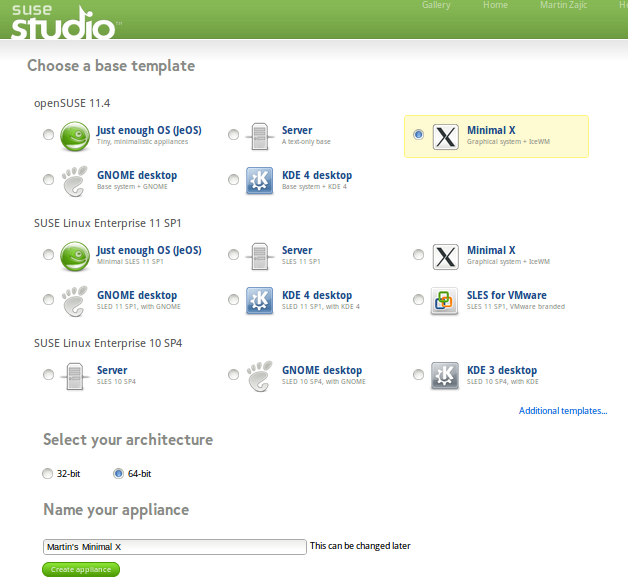
\includegraphics[width=3in]{./img/screens/suse2.png} &
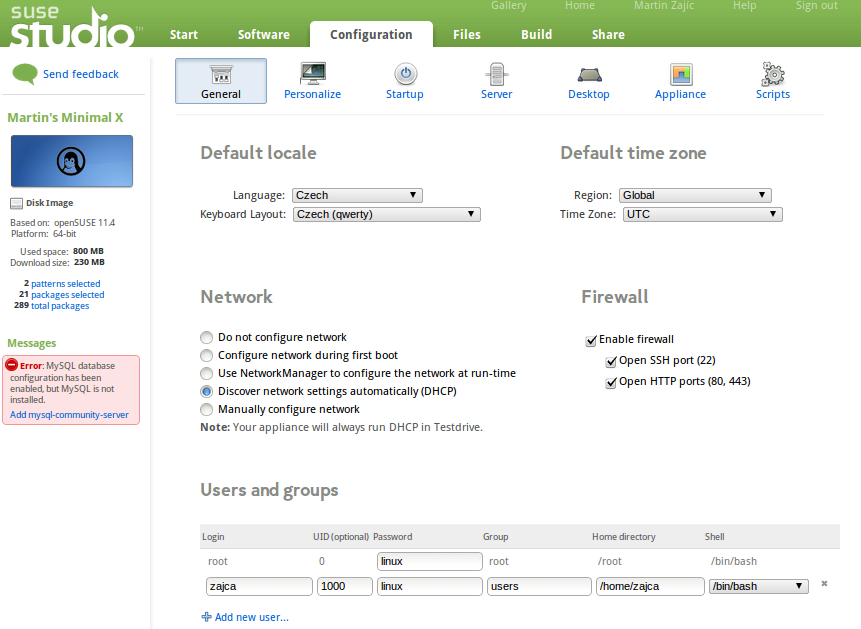
\includegraphics[width=3in]{./img/screens/suse3.png}
\end{array}$
\end{center}
\caption{Webové rozhraní s nastavením systému, vlevo výběr základního rozhraní, vpravo podrobnější nastavení}
\end{figure}

%\begin{center}
%\obr{./img/screens/suse1.png}{0.5}{Grafické rozhraní programu Revisor}
%\end{center}
%\begin{center}
%\obr{./img/screens/suse2.png}{0.5}{Grafické rozhraní programu Revisor}
%\end{center}
%\begin{center}
%\obr{./img/screens/suse3.png}{0.5}{Grafické rozhraní programu Revisor}
%\end{center}
\newpage
\nadpis{Pungi}\\
Pungi je nástrojem, který používají vývojáři Fedory pro sestavení oficiálních vydání. Jedná se o~program bez grafického rozhraní napsaný v~pythonu a~stejně jako Revisor stahuje balíčky z~internetu a sestavuje z~nich instalační médium.\cite{Linux_Build}

%This is the tool that the Fedora developers use to spin the official releases. It's a command-line tool written in Python.
%Like Revisor, the tool gathers packages directly from the internet and then automatically splits them and creates CD-sized installable ISO images.

\nadpis{Builder}\\
Builder je série skriptů napsaných v~BASHi, které používají vývojáři derivátu distribuce Ubuntu "gNewSense" na sestavení jejich distribuce. Ke skriptům je také napsán přehledný manuál jak je používat, který je dostupný online~\cite{Linux_Build}~\cite{BuilderNavod}.

%Builder is a series of bash scripts that are used by the gNewSense developers to create their distro. Along with the tool they've also written a handy nine-step guide to creating a customised distro from Ubuntu Hardy. The guide is available on their site.

\nadpis{MySlax Creator}\\
MySlax Creator jsou skripty určené k~úpravě distribuce Slackware, především tedy k~vytvoření vlastního obrazu odvozené distribuce SLAX. Jejich odlišnost je v~tom, že~fungují přímo z Windows.

%Here's a Slackware customisation script with a unique twist. The tool creates customised versions of the Slackware-based Slax distro we mentioned above, but unlike the other tools we talk about here, MySlax Creator installs and work from within Windows!
%It works with Slax ISO images and lets you add data to your own custom spins.

%\nadpis{LinuxCOE}\\
\newpage
\nadpis{Instalinux}\\ \label{sec:Instalinux}
Jednoduchým, ale mocným nástrojem je Instalinux, umožňuje uživateli vybrat z několika distribucí (Debian, Ubuntu, CentOS, Fedora, OpenSUSE, Scientific) a~v~dalších krocích základní nastavení systému a~výběr aplikací. Výsledkem je ISO obraz, kterým nemusí mít ani 30MB. Pro podrobnější nastavení existuje Designer Pro, který umožňuje nastavit mnohem více. Výbornou vlastností je uložení profilu, který je možné použít znovu a~upravit si jej.\\

%This is a simple, easy way to install Linux. You follow the steps in the System Designer to choose from a bunch of different distributions and versions of Linux, and to choose what software you want included. The final product will be a fairly small ISO image (30 MB or less) that you can burn to a CD and boot from. It will automatically build your system for you, pulling what it needs from the network mirror you selected, while you sit back and relax.

\begin{figure}[h]
\begin{center}$
\begin{array}{cc}
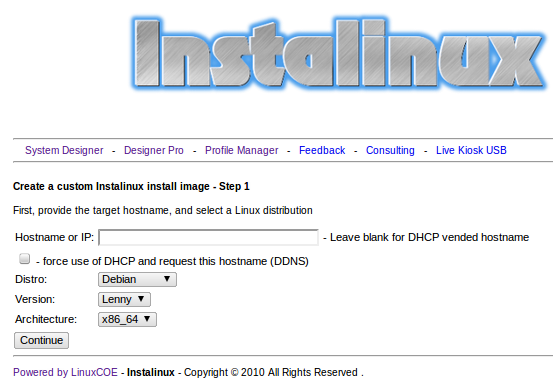
\includegraphics[scale=0.5]{./img/screens/instalinux1.png} &
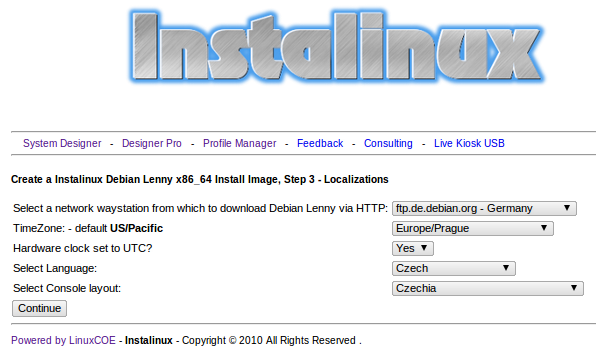
\includegraphics[scale=0.5]{./img/screens/instalinux2.png}
\end{array}$
\end{center}
\caption{Webové rozhraní Instalinux, vlevo výběr distribuce, vpravo nastavení jazyka a~časové zóny}
\end{figure}
\begin{figure}[h]
\begin{center}$
\begin{array}{cc}
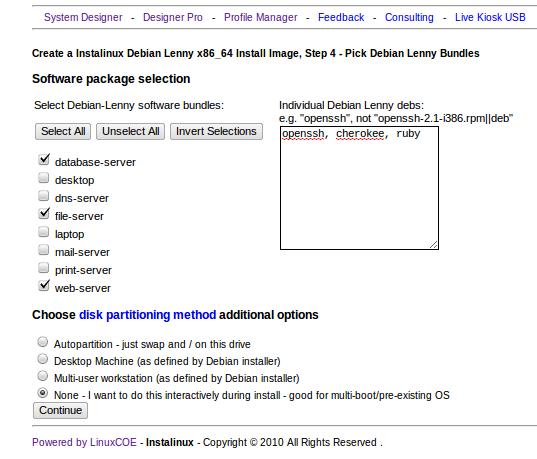
\includegraphics[scale=0.5]{./img/screens/instalinux3.png} &
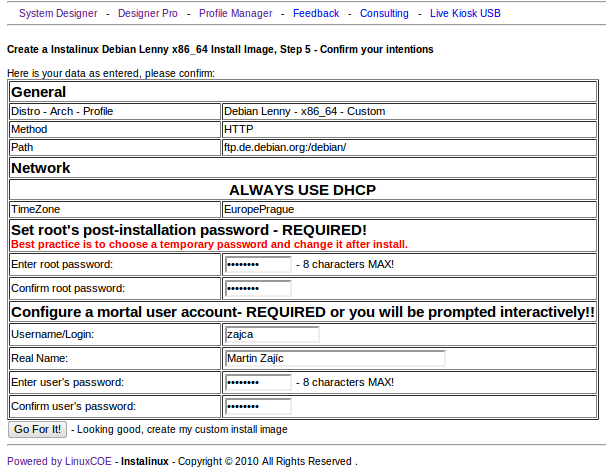
\includegraphics[scale=0.5]{./img/screens/instalinux4.png}
\end{array}$
\end{center}
\caption{Webové rozhraní Instalinux, vlevo výběr aplikací, vpravo nastavení uživatelů}
\end{figure}
Takto vytvořená distribuce může mít i~8MB!

\section{\upc{LiveCD}}
Ač by se mohlo zdát, že liveCD je nějaká velmi složitá věc k~vytvoření není to tak úplně pravda. Nejjednodušší forma LiveCD je taková, že vložíme CD do mechaniky, ten nabootuje a~spustí se příkazový řádek ve kterém je možné pracovat. Takto fungovaly a~často ještě fungují instalační CD různých distribucí. Dnes se velmi často používá několik druhů instalačních/live CD
\begin{itemize}
 \item Instalační CD s~příkazovou řádkou a~instalací pomocí textového nástroje (Archlinux,…)
 \item Instalační CD s~grafickým instalátorem (Debian,…)
 \item LiveCD ve kterém lze z~grafického Live prostředí spustit instalátor (ve většině případů lze spustit grafický isntalátor i~bez grafického live prostředí jako v~předchozí položce) (Ubuntu,…)
 \item Čistě LiveCD, takový disk slouží pouze pro vyzkoušení většinou grafického prostředí nebo k~opravám stávajícího systému (neobsahuje instalátor) (GNOME Live Media, Gparted,…)
 \item LiveCD určené pro běžnou práci. Takové LiveCD umí např. nahrát systém do RAM, pak už není třeba číst z~CD nebo také pokud se jedná o~LiveUSB je možné uložit změny v~systému na disk a~ty jsou načteny při dalším spuštění. (Slax,Chakra,…)
\end{itemize}

\subsection{Výhody/nevýhody LiveCD}
Vyhodou LiveCD je především možnost \textbf{vyzkoušet si celý operační systém bez nutnosti instalace}. Kompromisem LiveCD je pak \textbf{rychlost}, která se odvíjí od rychlosti čtení CD/DVD mechaniky. Rychlost LiveCD je možné zvýšit použitím jiného média než CD nebo DVD, např. použitím FlashDisku. Rychlost běhu lze zvýšit také \textbf{nahráním celého systému do paměti RAM}, tento proces má však velkou nevýhodu v~délce trvání, protože celé LiveCD musí být přečteno a~zapsáno do paměti RAM. Další nevýhodou je, až~na výjimky, nemožnost uložení změn v~systému zpět na přenosné médium.\\

Samozřejmě LiveCD není většinou používáno k~běžně práci, jeho výhodou je vyzkoušení neznámého operačního systému nebo grafického prostředí bez nutnosti mnohdy zdlouhavé instalace, což převyšuje nad nevýhodami.
\subsection{Možnosti tvorby LiveCD}
Vytvořit LiveCD lze několika způsoby, nejjednodušší je způsob úpravy stávajícího LiveCD jak bylo i~popsáno \odkazNaKapitolu{sec:tvorbaDistribuce}. 

\subsubsection{Obecný postup tvorby LiveCD}
Obecný postup tvorby LiveCD se dá shrnout do několika kroků.
\begin{enumerate}
 \item Vytvoření adresářové struktury LiveCD
 \item Připojení Virtual File System (VFS), ten zahrnuje složky: /sys /proc /dev /dev/shm /dev/pts /var/run
 \item Nainstalování základních balíčků
 \item Nainstalování modulů squashfs a~aufs
 \item Nainstalování kernelu a~vytvoření initramfs pomocí mkinitcpio s~minimálně aktivovanými moduly aufs, squashfs a loop, které jsou potřebně pro běh LiveCD.
 \item Nainstalování a~nastavení bootloaderu (GRUB)
 \item Doinstalování dalších balíčků
 \item Komprimace a~vytvoření squashfs souboru pomocí programu mksquashfs
 \item Vytvoření iso obrazu pomocí programu genisoimage, který vytvoří i~zaváděcí tabulku disku.
\end{enumerate}

\subsubsection{NimbleX}
Dalším nástrojem je jednoduchá webová aplikace na vytvoření vlastního derivátu NimbleX. Umožňuje vytvořit vlastní LiveCD obraz několik jednoduchými kroky, na výběr je stáhnutí minimálního obrazu nebo sestavení vlastního obrazu. U vlastního obrazu si uživatel vybere aplikace přehledně rozdělené do kategorií, wallpaper, nastavení zvuku, nastavení uživatelů a jazyk systému. Pak už jen počká na vygenerování obrazu, který je následujících 12hodin ke stažení.
\begin{figure}[h]
\begin{center}$
\begin{array}{cc}
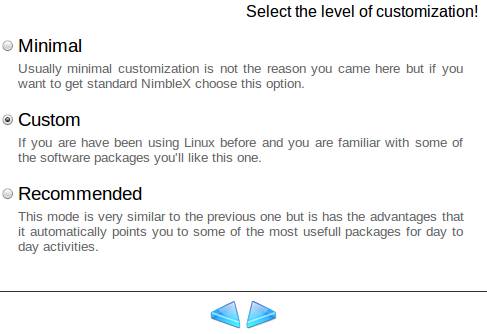
\includegraphics[width=2in]{./img/screens/nible1.png} &
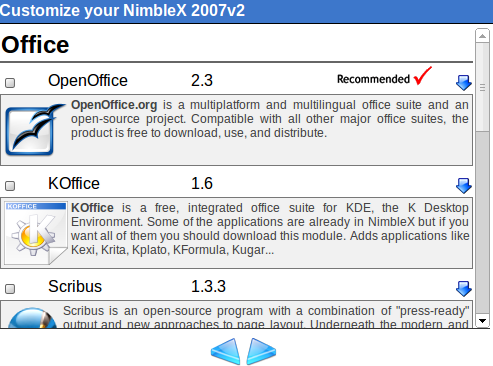
\includegraphics[width=2in]{./img/screens/nible2.png}
\end{array}$
\end{center}
\caption{Webové rozhraní s nastavením NimbleX, v levo výběr míry nastavení, v pravo nastavení programů v sekci office}
\end{figure}
\begin{figure}[h]
\begin{center}$
\begin{array}{cc}
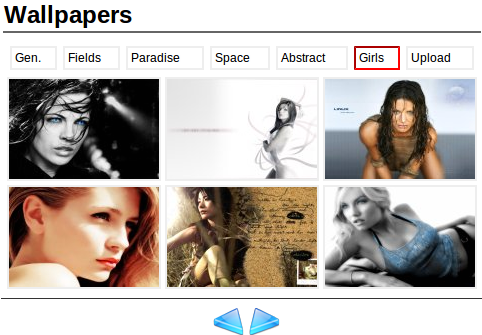
\includegraphics[width=2in]{./img/screens/nible3.png} &
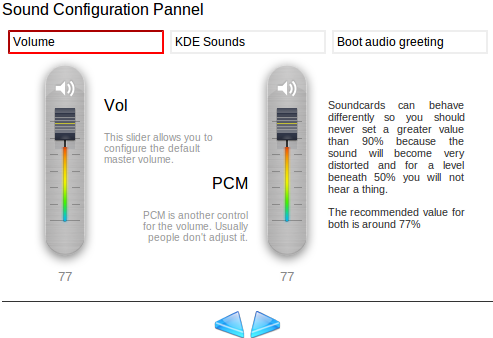
\includegraphics[width=2in]{./img/screens/nible4.png}
\end{array}$
\end{center}
\caption{Webové rozhraní s nastavením NimbleX, v levo výběr wallpaperu, v pravo nastavení zvuku}
\end{figure}

\subsubsection{Linux-Live}
Linux-Live je sada skriptů, která není závislá na distribuci, ale lze ji použít na jakémkoliv Linuxu. Prakticky stačí stáhnou skripty ze stránek Linux-Live a zkompilovat si kernel s podporou aufs a squashfs nebo si stáhnout již zkompilovaný kernel ze stránek Linux-Live. Skripty už pak samy vytvoří Live systém, který je možné nabootovat z CD nebo USB.

%If you want a truly distro-agnostic way of customising your favourite Linux distribution, you need the Linux-Live set of scripts. The scripts work on any installed Linux distro and can create a Live system that you can boot from optical media or USB drives.
%The popular Slackware -based Slax Live distro is built using these scripts, which work best on Slackware but can work on other distributions as well.

\subsubsection{Další možnosti tvorby LiveCD}
\b{Linux-Live} je asi nejčastějším způsobem vytvoření LiveCD. Spousta distribucí má, ale~vlastní nástroje některé jako: The Ubuntu Customisation Kit (UCK) nebo Reconstructor, které již byly popsány \odkazNaKapitolu{sec:UCK}. Pro fedoru např. exituje nástroj \b{livecd-creator} pro tvorbu Fedora LiveCD a~podrobný návod je dostupný na~stránkách fedory~\cite{FedoraLiveCDproject}. Pro debian existuje \textbf{Debian Live Project}, který poskytuje webové rozhraní podobné nástroji Instalinux \odkazNaKapitolu{sec:Instalinux} a~je zdarma dostupný na~internetu.~\cite{DebianLiveProject}
Další zajímavé nástroje pro tvorbu LiveCD existují např. pro~Archlinux. Jsou hned tři a~všechny jsou popsány na wiki stránkách distribuce Archlinux~\cite{ArchWiki-BuildLiveCD}. První je oficiální sada nástrojů, používaná k~tvorbě oficiálních vydání disků nazvaná \b{Archiso}. Druhým nástrojem je \b{larch}, který nepotřebuje k~sestavení jako hostitelský systém Archlinux, ale funguje v~jakémkoliv Linuxu, protože si potřebné aplikace stáhne z~repozitářů Archlinuxu. Posledním nástrojem je \textbf{poison-livecd-creator} jedná se o~opravdu jednoduchý Makefile a~několika jednoduchými kroky lze docílit vytvoření LiveCD na bázi Archlinuxu.


\section{\upc{Zabezpečení Linuxového systému}}

Zabezpečení OS je velice rozsáhlým a~komplexním odvětvím, které se navíc velmi rychle vyvíjí a~rozšiřuje. Jeho plné popsání by vydalo na několik desítek bakalářských prací, proto jen základní informace o~vnitřním zabezpečení systému, nástrojích jež toto zabezpečení rozšiřují a~také o~zabezpečení proti vnějšímu útoku a~bezpečném přenosu informací.

\subsection{Bezpečnostní model Linuxu}
Standardní bezpečnostní model, vycházející z~Discretionary Access Control (DAC) \odkazNaKapitolu{sec:DAC}, který nalezneme na většině UNIXových operačních systemů (tedy i~Linuxu) je postaven na několika bitových maskách (specifikující u souboru práva pro vlastníka, skupinu, ostatní (drwxrwxrwx) a~popř. nastavující některé speciální bity, jako je SUID (secure user identification number) či SGID (secure group identification number)). Další velmi typickou stránkou tohoto bezpečnostního modelu je uživatel root – administrátor a~uživatel s~nejvyššími možnými privilegii (jinak řečeno uživatel, jenž může vše).~\cite{LINUXZONEGrsecurity}\\

Tento bezpečnostní model se v~praxi v~různých UNIXových klonech osvědčil a~používá se dodnes. Ale jsou případy kdy není zrovna nevýhodnější. Prvním problémem jsou ona již zmíněná přístupová práva k~souborům, která jsou ze své podstaty poměrně omezená a~nastavení práv tak často nutí administrátora k~různým krokům, jako je např. vytváření velkého množství uživatelských skupin (a~v~některých případech ani~to není uspokojivým řešením).
Dalším kamenem úrazu je uživatel root, kterýžto jako administrátor prakticky má veškerá možná práva. Některý software část těchto práv ovšem vyžaduje – typickým příkladem je většina síťových démonů, které poslouchají na privilegovaných síťových portech (<1024). A~mimo oněch potřebných práv tak program zcela zbytečně dostane plnou kontrolu nad systémem, což může být zneužito potenciálním útočníkem, pokud se v~onom softwaru vyskytuje nějaká bezpečnostní chyba. Standardně se tento problém řeší tak, že program zahazuje EUID 0 (effective user identification number) v~momentě, kdy již nepotřebuje speciální práva.~\cite{LINUXZONEGrsecurity}\\

Dalším souvisejícím problémem je nemožnost efektivní distribuce práv k~systému mezi více administrátorů. Příkladem budiž situace, v~níž potřebujeme svěřit administraci DNS serveru jinému člověku než tomu, který se stará o~zbytek administrace systému. Nasnadě je povolení zápisu do konfiguračních souborů onoho daemonu, ale~tím vyřešíme jen část problémů. Onen administrátor též musí mít možnost např. onen server restartovat či mu alespoň poslat nějaký signál (např. pro načtení nové konfigurace), což s~sebou přináší nutnost superuživatelských práv. Jistým řešením je sudo či podobný nástroj, který umožňuje administrátorovi nastavit, jaké příkazy (a~pod jakým uživatelem) může daný uživatel spouštět ze svého normálního uživatelského účtu. Nicméně nejedná se o~dostatečně flexibilní řešení.~\cite{LINUXZONEGrsecurity}\\

Řešení se nabízí pomocí bezpečnostních patchů linuxového jádra implementující jiné modely přístupu než je v~Linuxu standardní Discretionary Access Control (DAC).

\subsection{Access Control}

Kontrola přístupu uvnitř systému je jedno z~nejdůležitějších zabezpečení v~OS vůbec. Určuje, který proces nebo uživatel má k čemu oprávnění. Existuje několik obecných modelů tohoto zabezpečení. V~Linuxu se konkrétně využívá modelu \b{Discretionary Access Control (DAC)}, který je standardní součástí Linuxového jádra.

%\subsubsection{Linux Security Module (LSM)} představuje nový mechanismus v~jádrech 2.6.x, který umožňuje jaderným modulům převzít kontrolu nad některými rozhodovacími mechanismy jádra. Přítomnost tohoto mechanismu je velmi významná pro zlepšení flexibility bezpečnostních mechanismů v~Linuxu, na druhou stranu LSM též sklidilo poměrně silnou kritiku od autorů jiných bezpečnostních patchů (grsecurity, RSBAC) a~ani jeden z těchto projektů nehodlá v~budoucnu využívat možností LSM, které se autorům oněch projektů jeví jako nedostačující.~\cite{LINUXZONEGrsecurity}\\

\subsubsection{DAC vs. MAC vs. RBAC} \label{sec:DAC}

Bezpečnostní model využívaný většinou mainstreamových operačních systému je založen na \b{Discretionary Access Control (DAC)}, který je založen na bezpečnosti vlastnictvím. Pokud uživatel vlastní soubor, může nastavovat práva pro čtení, zápis a~spouštění (r+w+x), pro tento soubor. V~tomto modelu uživatel kontroluje data dle vlastního uvážení. Vlastník systému\footnote{Vlastník systému (anglicky system owner nebo také administrátor) je určen při instalaci OS, oproti účtu uživatele root nemá právo měnit např. práva systémových souborů, ale má právo měnit přístupová práva široké škály uživatelů a~uživatelé nemají možnost tato ustanovení měnit.\cite{SystemOwner}} nemá totální kontrolu nad systémem, tu má uživatel.~\cite{Linux_com_MACvsDAC}


V Mandatory (česky Povinné) Access Control (MAC), uživatelům jsou dána povolení ke~zdrojům správcem. Pouze správce může udělit oprávnění nebo právo k~objektům a~zdrojům. Přístup ke zdrojům je založený na úrovni zabezpečení objektu a uživateli je udělena bezpečnostní prověrka pro přistup k~objektu. Pouze správci mohou upravovat objektu bezpečnostní štítek nebo uživateli bezpečnostní prověrky.

V Role-Based Access Control (RBAC), je přístup ke zdrojům založen na \uv{roli kterou uživatel hraje}. V tomto modelu, správce přiřadí uživateli roli, která má předem přidělena určitá práva a~výsady. Vzhledem k~uživateli přidělené roli, může uživatel přístupovat k~určitým zdrojům a~plnit specifické úkoly. RBAC je také známý jako Non-Discretionary Access Control. Role přiřazené uživatelům, jsou centrálně spravovány.

\subsubsection{Security-Enhanced Linux, SElinux}

SELinux je bezpečnostní vylepšení pro Linux, které dává uživatelům a správcům větší kontrolu nad tím, který uživatele nebo aplikace může přistupovat k jakým prostředkům. Standardní Linuxová kontrola přístupu jako je oprávnění pro soubor (-rwxr-xr-x) je modifikovatelné uživatelem nebo aplikací, kterou uživatel spustí. Oproti tomu, kontrola přístupu v~SELinuxu je určena pravidly v~systému a~neopatrný uživatel nebo nesprávná aplikace je nemůže nijak změnit.

SELinux také přidává mnoho možností pro řízení přístupu. Místo klasického určení, kdo může číst, psát nebo spustit soubor, např. SELinux umožňuje určit, kdo může vytvářet a~rušit odkazy, přesouvat soubory a~mnoho dalšího. SELinux umožňuje určit přístup k mnoha jiným zdrojům než jen k souborům, např. přístup k~síťovým zdrojům nebo k~mezi procesové komunikaci (IPC).\cite{SElinuxWiki}

%SELinux is a security enhancement to Linux that allows users and administrators more control over which users and applications can access which resources, such as files. Standard Linux access controls, such as file modes (-rwxr-xr-x) are modifiable by the user and applications that the user runs whereas SELinux access controls are determined by a policy loaded on the system and not changeable by careless users or misbehaving applications.
%SELinux also adds finer granularity to access controls. Instead of only being able to specify who can read, write or execute a file, for example, SELinux lets you specify who can unlink, append only, move a file and so on. SELinux allows you to specify access to many resources other than files as well, such as network resources and interprocess communication (IPC).

\subsubsection{AppArmor}

AppArmor je efektivní a~snadno použitelná Linuxová bezpečnostní aplikace. AppArmor aktivně chrání operační systém a~aplikace před vnějšími nebo vnitřními bezpečnostními hrozbami a~díky prosazování dobrého chování a~prevence od neznámých, nebezpečných nebo vadných aplikací dokáže chránit systém i~od tzv. zero-day útoků\footnote{zero-day atack je útok na vývojářům neznámou zranitelnost~v systému. Zero-day je také nazýván, protože se objeví dříve než vývojáři dokáží chybu záplatovat.}. V~bezpečnostních pravidlech AppArmor lze definovat, k~jakým systémovým zdrojům můžou jednotlivé aplikace přistupovat a~jak s nimi mohou nakládat. Mnoho výchozích bezpečnostních pravidel je součástí AppArmor a~pomocí kombinace vyspělé statické analýzy a~learning-based nástrojů, je možné bezpečnostní pravidla AppArmor i~pro velmi složité aplikace úspěšně nasadit během několika hodin.\cite{AppArmorWikiMain}

AppArmor se především oproti SElinuxu vyznačuje mnohem jednodušším nastavením.
%AppArmor is an effective and easy-to-use Linux application security system. AppArmor proactively protects the operating system and applications from external or internal threats, even zero-day attacks, by enforcing good behavior and preventing even unknown application flaws from being exploited. AppArmor security policies completely define what system resources individual applications can access, and with what privileges. A number of default policies are included with AppArmor, and using a combination of advanced static analysis and learning-based tools, AppArmor policies for even very complex applications can be deployed successfully in a matter of hours.

\subsubsection{TOMOYO}

Tomoyo Linux je Mandatory Access Control (MAC) implementace pro Linux, díky které lze zvýšit zabezpečení systému a~nebo může být pouze nástrojem systémové analýzy. Jeho vývoj byl zahájen v~březnu 2003 a je sponzorován NTT Data Corporation, Japonsko.

Tomoyo Linux se zaměřuje na chování systému. Každý proces je vytvořen za dosažením určitého cíle a~jako imigrační pracovník, Tomoyo Linux umožňuje každému procesu určit si zdroje potřebné k~dosažení svého cíle. Pokud je povolena ochrana, Tomoyo Linux funguje jako hlídací pes a~omezuje každý proces tak, jak má povoleno správcem.\cite{TOMOYOLinuxHOME}

Mezi hlavní přednosti Tomoyo Linux patří:
\begin{itemize}
 \item Systémová analýza
 \item Zvýšená bezpečnost díky Mandatory Access Control (MAC)
 \item Nástroje na podporu generování bezpečnostních pravidel
 \item Jednoduché syntaxe
 \item Snadné použití
 \item Velmi málo závislostí
 \item Nevyžaduje žádné úpravy stávajících spustitelných souborů.
\end{itemize}

%TOMOYO Linux is a Mandatory Access Control (MAC) implementation for Linux that can be used to increase the security of a system, while also being useful purely as a system analysis tool. It was launched in March 2003 and is sponsored by NTT DATA Corporation, Japan.

%TOMOYO Linux focuses on the behaviour of a system. Every process is created to achieve a purpose, and like an immigration officer, TOMOYO Linux allows each process to declare behaviours and resources needed to achieve their purpose. When protection is enabled, TOMOYO Linux acts like an operation watchdog, restricting each process to only the behaviours and resources allowed by the administrator.

%The main features of TOMOYO Linux include:
%System analysis
%Increased security through Mandatory Access Control
%Tools to aid in policy generation
%Simple syntax
%Easy to use
%Very few dependencies
%Requires no modification of existing binaries

\subsubsection{grsecurity}

grsecurity je inovativní přístup k~zabezpečení, využívající multi-layered (vícevrstvou) detekci, prevenci a omezení modelu. Je vyvíjen pod licencí GNU GPL.~\cite{Grsecurity}

Nabízí mnoho funkcí:
\begin{itemize}
 \item inteligentní a robustní Role-Based Access Control (RBAC) systém, který může generovat bezpečnostní pravidla pro celý systém bez jakékoliv konfigurace
 \item Rozsáhlé kontroly
 \item Prevence nežádoucího kódu, bez ohledu na použité techniky (stack smashing, heap corruption, atd…)
 \item Prevence spuštění libovolného kódu v jádře
 \item Randomizaci zásobníku a knihoven
 \item Ochrana proti využitelným chybám null-pointer dereference~\cite{Null-pointerDereference} v jádře
 \item Snížení rizika úniku citlivých informací díky chybám v jádru systému
 \item Omezení, která umožňují uživateli zobrazit pouze své procesy
 \item Výstrahy zabezpečení a audity, které obsahují IP adresu osoby, která způsobila záznam
\end{itemize}


%grsecurity is an innovative approach to security utilizing a multi-layered detection, prevention, and containment model. It is licensed under the GNU GPL.
%It offers among many other features:
%An intelligent and robust Role-Based Access Control (RBAC) system that can generate least privilege policies for your entire system with no configuration
%Change root (chroot) hardening
%/tmp race prevention
%Extensive auditing
%Prevention of arbitrary code execution, regardless of the technique used (stack smashing, heap corruption, etc)
%Prevention of arbitrary code execution in the kernel
%Randomization of the stack, library, and heap bases
%Kernel stack base randomization
%Protection against exploitable null-pointer dereference bugs in the kernel
%Reduction of the risk of sensitive information being leaked by arbitrary-read kernel bugs
%A restriction that allows a user to only view his/her processes
%Security alerts and audits that contain the IP address of the person causing the alert


\subsection{Hodnocení bezpečnosti OS a SW}

Tak jako ve spoustě jiných odvětvích se i~v~bezpečnosti určují standardy a~udělují certifikace bezpečnosti.

\subsubsection{Trusted Computer System Evaluation Criteria, TCSEC} \label{sec:TCSEC}

Asi nejznámější kniha popisující požadavky pro "důvěryhodný" operační systém, vydaná v roce 1985 americkým ministerstvem obrany (Department of Defense, DoD) a je známa také jako oranžová kniha (Orange book) pro svůj oranžový přebal. Dnes se tyto hodnotící kritéria již nepoužívají, původně měla být nahrazena Federal Criteries (FC), ale tento soubor kritérií nebyl nikdy nasazen a zůstal pouze ve fázi draft\footnote{\b{Draft} se používá jako označení pro návrh}, protože jej v roce 2005 nahradil soubor Common Criteria (CC) \odkazNaKapitolu{sec:cc}\\

\vspace{4 mm}
TCSEC, hodnotí míru splnění požadavků ve třech oblastech informační bezpečnosti~\cite{PrezentaceBIS}
\begin{description}
 \item[Zásady (Policy)] metody řízení přístupu, označení stupně utajení
 \item[Odpovědnost (Accountability)] zjištění identity uživatele, monitoring činnosti uživatele
 \item[Záruky (Assurance)] požadavky na nezávislé hodnocení a průběžné provádění bezpečnostních funkcí
 \end{description}
\b{Seznam tříd bezpečnosti operačního systému podle TCSEC:}
\begin{description}
\item[Třída D] minimální ochrana - systémy nevyhovující vyšším třídám
\item[Třída C] výběrová ochrana (Discretionary Protection) prosazuje výběrové řízení přístupu
\begin{description}
\item[Podtřída C1] ochrana s výběrovým přístupem - základní oddělení uživatelů a~dat chrání citlivá data před náhodným zneužitím
\item[Podtřída C2] ochrana  s řízeným přístupem - detailnější řízení přístupu a audit činností
\end{description}
\item[Třída B] povinná ochrana (Mandatory Protection)
\begin{description}
\item[Podtřída B1] ochrana bezpečnosti návěštím - přidělení stupně utajení (neformální model)
\item[Podtřída B2] strukturovaná ochrana - existence polo-formálního modelu, oddělení citlivých a necitlivých částí systému (odolnost proti napadení)
\item[Podtřída B3] bezpečnostní domény - modulární architektura systému (vysoká odolnost proti napadení)
\end{description}
\item[Třída A] verifikovaná ochrana (Verified Protection)
\begin{description}
\item[Podtřída A1] verifikovaný návrh funkčně stejně jako B3, rozšíření míry formální specifikace a verifikace při návrhu a testování 
\end{description}
\end{description}
Systémy třídy A se mezi komerčně dostupnými produkty nevyskytují\\
Systémy s dostatečnou bezpečností pro běžný provoz se považují systémy minimálně třídy C2~\cite{PrezentaceBIS}\\
Většina Linuxových distribucí dosahuje Třídy C2~\cite{LinuxDictionary}

\subsubsection{IT Security Evaluation Criteria,ITSEC}\label{sec:ITSEC}

Evropská kritéria vytvořená v roce 1990 dnes již nahrazena kritérii Common Criteries (CC)~\odkazNaKapitolu{sec:cc}.

Rozdělení požadavků kladených na
\begin{itemize}
 \item Předmět hodnocení
 \item Míru záruk a funkčnost
\end{itemize}
Třídy záruk za správnost (E0-E6) a~efektivnost odolat možným útokům~\cite{PrezentaceBIS}
\begin{description}
 \item[E0] požadavky ITSEC nesplněny
 \item[E1] požadavek na neformální zadání bezpečnosti a popis návrhu a důkazní testy
 \item[E2] požadavek na neformální popis detailního návrhu, nezávislé testy
 \item[E3] jako třída E2 a hodnocení zdrojového kódu (SW) nebo obvodových schémat (HW)
 \item[E4] formální model bezpečnostního návrhu a provedení analýzy zranitelnosti
 \item[E5] požadavek na specifikaci návaznosti detailního návrhu a zdrojových kódů (schémat)
 \item[E6] jako třída E5 a formální popis návrhu a doložení jeho konzistence s matematickým modelem. 
\end{description}

Třídy funkčnosti~\cite{PrezentaceBIS}
\begin{description}
\item[F-C1 až F-B3] podle TCSEC 
\item[F-IN] vysoké nároky na integritu
\item[F-AV] vysoké nároky na dostupnost
\item[F-DI] vysoké nároky na integritu při přenosu
\item[F-DC] vysoké nároky na důvěrnost při přenosu
\item[F-DX] vysoké nároky na důvěrnost a integritu při přenosu
\end{description}

\subsubsection{Canadian Trusted Computer Product Evaluation Criteria, CTCPEC}\label{sec:CTCPEC}

Kanadský soubor kriterií, který je dnes již také nahrazen Common Criteries (CC)~\odkazNaKapitolu{sec:cc}.\\

Hodnocený systém je chápán jako soubor bezpečnostních funkcí s úrovní záruk~\cite{PrezentaceBIS}\\

Funkce - rozdělení do skupin, v každé skupině pro každou funkci je stanoveno několik úrovní~\cite{PrezentaceBIS}
\begin{description}
 \item[Skupina C - "Důvěrnost"] 4 funkce, ochrana proti úniku informace 
 \item[Skupina I - "Integrita"] 7 funkcí pro udržení konsistence dat a systému 
 \item[Skupina A - "Dostupnost"] 4 funkce pro udržení dosažitelnosti služeb 
 \item[Skupina W - "Odpovědnost"] 3 funkce pro zajištění odpovědnosti uživatelů 
\end{description}

\subsubsection[Common Criteria, CC]{Common Criteria for Information Technology Security Evaluation, CC}\label{sec:cc}

V České republice je dobře známa norma ISO/IEC 15408-1:1999, která je totožná s~textem, zveřejněným Organizacemi sponzorujícími projekt Společná kritéria, pod názvem “Common Criteria for Information Technology Security Evaluation”, verze 2.1. Tato kritéria jsou obvykle nazývána pouze “Common Criteria” a~pro jejich označení se hojně používá zkratky “CC”. Zkratka “CC”
je ponechána i~v~českém překladu normy.~\cite{NBUHodnoceniBezpecnostiSW}

V současné době se používá verze 3.0.

CC vznikla na základě již dříve používaných kritérií hodnocení, zejména amerických TCSEC~\odkazNaKapitolu{sec:TCSEC} a~Federal Criteria, evropských ITSEC~\odkazNaKapitolu{sec:ITSEC} a~kanadských CTCPEC~\odkazNaKapitolu{sec:CTCPEC}. Na vývoji CC se podílely národní organizace, působící v~oblasti bezpečnosti a~standardizace, z~šesti států světa, jmenovitě Kanady, Francie, Německa, Holandska, Velké Británie a~Spojených států amerických a~jsou posledním výsledkem úsilí o~vytvoření společného standardu v~oblasti hodnocení bezpečnosti informačních technologií. V~uvedených státech lze nalézt většinu z~uznávaných laboratoří, které prováděly hodnocení bezpečnosti produktů v~oblasti informačních technologií podle dříve široce akceptovaných kritérií TCSEC nebo ITSEC a~v~současné době již přešly výhradně na hodnocení podle CC.~\cite{NBUHodnoceniBezpecnostiSW}

Jako formální základ pro vzájemné uznávání hodnocení uzavřely Kanada, Francie, Německo, Velká Británie a Spojené státy americké v roce 1998 dohodu “Arrangement on the Recognition of
Common Criteria Certificates in the field of Information Technology Security”, zkráceně nazývanou CCRA (CC Recognition Arrangement).~\cite{NBUHodnoceniBezpecnostiSW}

\b{CC jsou rozdělena do 3 částí:}
\begin{description}
 \item[Část 1/ Part 1] Úvod a všeobecný model (Introduction and general model)
 \item[Část 2/ Part 2] Bezpečnostní funkční požadavky (Security functional requirements)
 \item[Část 3/ Part 3] Požadavky na záruky bezpečnosti (Security assurance requirements)
 \end{description}

V~\b{prvé části} jsou uvedeny definice pojmů, je vysvětlena základní filosofie CC a~je prezentován obecný model hodnocení. Důležitou součástí je vymezení několika stavebních prvků, které slouží pro jednotné vyjádření bezpečnostních požadavků, ať již funkčních nebo na záruku.~\cite{NBUHodnoceniBezpecnostiSW}\\

Jsou to:
\begin{description}
 \item[prvek (element)] jako dále nedělitelný bezpečnostní požadavek ověřitelný při hodnocení
 \item[komponenta (component)] jako nejmenší množina prvků pro zahrnutí do vyšších struktur v~CC
 \item[rodina (family)] jako seskupení komponent, z~nichž všechny slouží k naplnění téhož cíle, ale~liší se přísností požadavků
 \item[třída (class)]jako seskupení rodin, které pokrývají jednotlivé dílčí cíle a~dohromady tvoří konsistentní celek pro dosažení určitého cíle celkového
 \end{description}

Důležitým pojmem v CC je \b{“profil ochrany” (Protection Profile, PP)}, který představuje implementačně nezávislou množinu bezpečnostních požadavků pro zajištění definovaných cílů. Tyto požadavky mohou být vybrány z~CC nebo být vyjádřeny explicitně a~mají zahrnovat i~míru záruky hodnocení (Evaluation Assurance Level, EAL). PP se obvykle vytváří tak, aby byl opakovatelně použitelný a~musí obsahovat i~zdůvodnění bezpečnostních cílů a~požadavků.~\cite{NBUHodnoceniBezpecnostiSW}

Pokud jde o~specifický produkt nebo~systém, nazývaný \b{“předmět hodnocení” ( Target of Evaluation, TOE)}, vyjadřují se bezpečnostní požadavky, které~jsou v~něm realizovány, jako tzv. \b{“bezpečnostní cíl” (Security Target, ST)}. ST je množinou bezpečnostních požadavků, vyjádřených odkazem na PP, na~existující balíky, na~komponenty CC nebo explicitně.~\cite{NBUHodnoceniBezpecnostiSW}

Ve \b{druhé části} jsou stanoveny funkční komponenty, které~budou používány jako standardní způsob vyjadřování funkčních požadavků. Jde v~podstatě o~katalog funkčních komponent, rodin a~tříd.~\cite{NBUHodnoceniBezpecnostiSW}\\
Je definováno 11 funkčních tříd, jejichž originální anglické názvy/české názvy jsou:
\begin{itemize}
 \item Audit/Bezpečnostní audit
 \item Identification and Authentication/Identifikace a autentizace
 \item Resource Utilisation/Využití zdrojů
 \item Cryptographic Support/Kryptografická podpora
 \item Security Management/správa bezpečnosti
 \item TOE Access/Přístup k TOE
 \item Communications/Komunikace
 \item Privacy/Soukromí
 \item Trusted Path/Channels / Důvěryhodná cesta/kanály
 \item User Data Protection/Ochrana uživatelských dat
 \item Protection of the TOE Security Functions/Ochrana TSF
\end{itemize}

\b{Třetí část} zahrnuje komponenty pro popis požadavků na záruky. Je katalogem komponent záruk, jejich rodin a~tříd. Rovněž jsou v~ní definována kritéria pro hodnocení profilů ochrany (PP) a~bezpečnostních cílů (ST). V~CC je pro oblast záruk definováno 8 tříd, jejichž originální anglické názvy/české názvy jsou~\cite{NBUHodnoceniBezpecnostiSW}:
\begin{itemize}
 \item Configuration Management/Správa konfigurace
 \item Guidance Documents/Průvodní dokumentace
 \item Vulnerability Assessment/Posouzení zranitelnosti
 \item Delivery and Operation/Dodání a provoz
 \item Life Cycle Support/Podpora životního cyklu
 \item Assurance Maintenance/Údržba záruky
 \item Development/Vývoj
 \item Tests/Testy
\end{itemize}

Důležité je stanovení předdefinované vzestupné stupnice pro úroveň hodnocení. CC poskytuje 7 předdefinovaných balíků pro záruky (assurance package), známých jako Evaluation Assurance Levels (EAL), v~českém překladu míry záruky hodnocení. Jsou dobře promyšlené a~vyvážené, obecně aplikovatelné. Analogii lze nalézt v~třídách E1 až E6 v~kritériích ITSEC. Veškerá hodnocení IT podle CC se dnes provádějí na úrovni některé z~EAL, převážně do úrovně EAL4.~\cite{NBUHodnoceniBezpecnostiSW}\\

Stručně lze jednotlivé úrovně popsat následujícím způsobem:
\begin{description}
 \item[EAL1] je vhodná, pokud je vyžadována určitá základní důvěra ve~správnost fungování hodnoceného PP, ST nebo TOE, avšak hrozby nejsou považovány za vážné. Důvěry se dosahuje nezávislým testováním shody hodnoceného PP, ST nebo TOE s~neformální funkční specifikací a~zkoumáním předložených příruček pro uživatele.~\cite{NBUHodnoceniBezpecnostiSW}
 \item[EAL2] již vyžaduje spolupráci vývojáře, který musí v~podstatě dodat funkční specifikace, určité informace o návrhu bezpečnostních funkcí (na úrovni globálního návrhu, high-level design) a~výsledky testování, avšak vývoj si nevyžaduje více úsilí nežli je potřebné pro dodržování dobré komerční praxe, a~v~podstatě nepřináší zvýšení nákladů. Poskytuje nízkou až střední nezávisle ověřenou bezpečnost v~případě, že~není dostupná kompletní informace z~fáze vývoje. Důvěry se dosahuje analýzou vyžadované dokumentace, ověřením výsledků některých testů, analýzou síly funkcí a~analýzou zřejmých zranitelností. Pro TOE musí být sestaven seznam konfigurace a~vypracovány procedura pro bezpečnou instalaci, generování a~spouštění.~\cite{NBUHodnoceniBezpecnostiSW}
 \item[EAL3] je možno ještě dosáhnout bez podstatných změn základních existujících vývojářských praktik. Je aplikovatelná v~případě, že se vyžaduje střední úroveň nezávisle ověřené bezpečnosti a~je~opřena o~důkladné zkoumání TOE (ST, PP). Navíc oproti EAL2 se vyžaduje rozsáhlejší testování, kontroly vývojového prostředí a~zajištění správy konfigurace.~\cite{NBUHodnoceniBezpecnostiSW}
 \item[EAL4] stále umožňuje pohybovat se v~rámci dobré komerční vývojářské praxe. Jakkoliv přísné jsou tyto praktiky, nevyžadují podstatné specializované znalosti, dovednosti a~jiné zdroje. EAL4 je nejvyšší úrovní záruk, kterou lze dosáhnout (za rozumné náklady) zpětně pro již existující produkt. Poskytuje střední až vysokou úroveň záruky nezávisle ověřené bezpečnosti pro běžnou komoditu produktů a~vyžaduje ze strany vývojáře nebo~uživatelů připravenost k~pokrytí dodatečných specifických nákladů spjatých s~bezpečnostním inženýrstvím. Navíc oproti EAL3 se již vyžaduje také detailní návrh (low-level design) TOE, neformální model bezpečnostní politiky TOE a~dodání určité podmnožiny implementace (např. část zdrojového kódu bezpečnostních funkcí). Nezávislá analýza zranitelností musí demonstrovat odolnost vůči průniku útočníků s~nízkým potenciálem pro útok. Kontroly vývojového prostředí jsou doplněny modelem životního cyklu, stanovením nástrojů a~automatizovanou správou konfigurace.~\cite{NBUHodnoceniBezpecnostiSW}
 \item[EAL5]vyžaduje kromě přísného uplatnění dobré komerční vývojářské praxe aplikaci speciálních technik bezpečnostního inženýrství ve středním rozsahu. Dané TOE bude pravděpodobně již navrženo a~vyvíjeno s~cílem dosáhnout úrovně záruk EAL5. Nepředpokládá se nicméně velké zvýšení nákladů oproti EAL4. EAL5 je tak vhodná v~případech, kdy se vyžaduje vysoká úroveň záruky nezávisle ověřené bezpečnosti aniž by náklady na specializované techniky byly nerozumně vysoké. Navíc oproti EAL4 je vyžadováno dodání kompletní implementace TOE, formální model bezpečnostní politiky TOE, poloformální presentace funkčních specifikací, poloformální globální návrh (high-level design) a~poloformální demonstrace korespondence. Nezávislá analýza zranitelností musí demonstrovat odolnost vůči průniku útočníků se středním potenciálem pro útok. Vyžaduje se také analýza skrytých kanálů a~modularita návrhu.~\cite{NBUHodnoceniBezpecnostiSW}
 \item[EAL6] vyžaduje aplikaci technik bezpečnostního inženýrství do přísného vývojového prostředí a~je určena pro vývoj TOE sloužícího pro ochranu vysoce hodnotných aktiv proti význačným rizikům, kdy lze odůvodnit dodatečné náklady. Navíc oproti EAL5 se vyžaduje poloformální detailní návrh, rozsáhlejší testování, návrh TOE musí být modulární a~zvrstvený, prezentace implementace strukturovaná. Nezávislá analýza zranitelností musí demonstrovat odolnost vůči průniku útočníků s~vysokým potenciálem pro útok. Analýza skrytých kanálů musí být systematická. Vyšší nároky jsou kladeny na~správu konfigurace a~kontroly vývojového prostředí.~\cite{NBUHodnoceniBezpecnostiSW}
 \item[EAL7] je použitelná pro vývoj produktů určených do extrémně rizikového prostředí a/nebo~kde vysoká hodnota aktiv ospravedlňuje vyšší náklady. Praktické použití EAL7 je v současnosti omezeno na~TOE a~úzce vymezenou bezpečnostní funkčností, kde lze provést formální analýzu v~požadované míře. Vyžaduje se plná formalizace, formální model bezpečnostní politiky, formální presentace funkčních specifikací and high-level návrhu, poloformální detailní návrh, formální a~poloformální demonstrace korespondence. Testování se vyžaduje na úrovni bílé skříňky (white-box) a~musí být dosaženo úplného nezávislého potvrzení výsledků všech předložených testů. Složitost návrhu musí být minimalizována.~\cite{NBUHodnoceniBezpecnostiSW}
\end{description}
Operační systém Linux dosahuje úrovně EAL4.~\cite{CCredhat}~\cite{CCsuse}

\subsection{Uživatelé a přihlášení}

Linux je multiuživatelským systémem a~model uživatelského oprávnění vychází z~modelu DAC \odkazNaKapitolu{sec:DAC}. Přihlášení uživatele probíhá podobně jako u~webových a~jiných služeb. Tedy uživatelské heslo není v~systému uloženo, ale~je uložen pouze jeho HASH,získaný pomocí funkce SHA1 (záleží na nastavení sytému), když se pak uživatel přihlašuje do systému, je z~jím zadaného hesla vygenerován HASH a~porovnán s~HASHem uloženým v~sytému. 

\subsubsection{Uložení uživatelů a hesel}
Uživatelské v~OS Linux jsou definováni v~souboru /etc/passwd a~jejich hesla jsou zabezpečena pomocí šifry SHA1 a~uchována v~souboru /etc/shadow, který je přístupný pouze uživateli root. 

\nadpis{/etc/passwd}

Základní databází uživatelů v~systému Linux je textový soubor /etc/passwd (angl. password file), v němž jsou uvedena platná uživatelská jména a~další k~nim přidružené informace. Každému uživateli odpovídá v~souboru jeden záznam - řádek, který je rozdělen na sedm polí, jejichž oddělovačem je dvojtečka. Význam jednotlivých položek je následující~\cite{LDP}:
\begin{enumerate}
 \item Uživatelské jméno.
 \item Pole pro heslo v~zakódované podobě, které se nepoužívá a~heslo se ukládá do /etc/shadow
 \item Identifikační číslo uživatele.
 \item Identifikační číslo pracovní skupiny (angl. group ID, zkráceně GID).
 \item Skutečné jméno uživatele, případně popis účtu.
 \item Domovský adresář.
 \item Příkazový interpret (nebo program), který se spustí po přihlášení.
\end{enumerate}

Každý uživatel systému má k~souboru /etc/passwd přístup (může jej číst). Může tedy například zjistit přihlašovací jména ostatních uživatelů~\cite{LDP}.\\

\nadpis{/etc/shadow}

Soubor /etc/shadow (nebo také-li soubor stínových hesel) uchovává hesla uživatelů v~zašifrované podobě pomocí definovaného šifrovacího algoritmu (nejčastěji MD5, DES nebo SHA1). Často se nepoužívá přímo šifra hesla, ale tzv. salt což je ochrana proti tzv. rainbow attacku (česky duhový útok) což je útok na HASHovací funkce pomocí tabulek hesel (rainbow tables) a~podobností v~nich. Salt (česky sůl) pak rozpouští duhu a~znemožňuje tak rainbow attack, díky přidání předdefinovaných stringů do hesla, které je pak zašifrováno.~\cite{rubyOnRailTutorial}\\

Můžou existovat tři druhy uživatelů podle možností přihlášení:
\begin{description}
 \item[Uživatel s heslem] běžný uživatel s~nastaveným heslem. Jeho nastavení vypadá asi takto:\\
/etc/passwd
    \begin{codeframe}
      \begin{Verbatim}{frame=single}
lfs:x:1002:1000::/home/lfs:/bin/bash
\end{Verbatim} 
    \end{codeframe}
/etc/shadow
    \begin{codeframe}
      \begin{Verbatim}{frame=single}
lfs:$1$MhyAxheU$Nq85ITaTmL8yJqgHXoOEK0:15111:0:99999:7:::
\end{Verbatim} 
    \end{codeframe}
 \item[Uživatel bez hesla] Běžný uživatel jehož přihlášení nevyžaduje heslo, \b{POZOR! je rozdíl jestli je uživatel bez hesla nebo se při startu systému přihlašuje uživatel automaticky prostřednictvím správce sezení jako je GDM nebo KDM}. Nastavení uživatele bez hesla se liší pouze v~souboru /etc/shadow a~heslo je nahrazeno prázdným stringem:\\
/etc/shadow
    \begin{codeframe}
      \begin{Verbatim}{frame=single}
lfs:$1$VNMbpxGH$sew7cnwH9ixU.x27UbFNn.:15111:0:99999:7:::
\end{Verbatim} 
    \end{codeframe}
\b{POZOR!!! takový přístup se nepoužívá! Uživatelé bez hesla se používají pouze na LiveCD!}
 \item[Uživatel bez přihlášení] uživatel bez přihlášení se používá pro služby (v~Linuxu daemony, česky někdy též démony), je to speciální druh uživatele, za kterého se nelze přihlásit a~používá se aby byla práva služeb oddělena od uživatelů a~neběžela pod oprávnění uživatele root. Jejich nastavení se liší od normálního uživatele pouze v~tom, že~v~souboru /etc/passwd je defaultní shell jako /bin/bash nahrazen /bin/nologin nebo /bin/false\\
/etc/shadow
    \begin{codeframe}
      \begin{Verbatim}{frame=single}
dbus:x:81:81:System message bus:/:/bin/false
\end{Verbatim} 
    \end{codeframe}
a~heslo v~/etc/shadow je nahrazeno vykřičníkem
    \begin{codeframe}
      \begin{Verbatim}{frame=single}
dbus:!:15084:0:99999:7:::
\end{Verbatim} 
    \end{codeframe}

 \end{description}

\subsubsection{Přihlášení uživatele}
Pro přihlášení uživatele se používá několik způsobů, ať už grafických textových nebo vzdálených.\\

Základní možnosti přihlášení uživatele:
\begin{description}
 \item[Computer terminal (tty)] Standardní přihlášení do systému, uživatel zadá uživatelské jméno, heslo a~je mu zpřístupněn systém prostřednictvím console.
 \item[Desktop manager] slouží jako přihlašovací obrazovka do většiny grafických prostředí a~většinou poskytuje kromě přihlášení, také služby jako je vypnutí, restart nebo uspání bez nutnosti zadání hesla uživatele root. Existují \textbf{grafické desktopové managery} jako KDM, GDM, SLiM, XDM, EDM, LightDM a~jiné. Velmi často se ke grafickému prostředí váže i~jeho vlastní desktop manager, který ovšem dokáže spouštět i~ostatní prostředí. \textbf{Textových desktopových managerů} existuje velmi málo a~většinou se jedná pouze o~nástroje, které umožní po textovém přihlášení spustit Xserver se zvoleným grafickým prostředím. wmctrl, CDM.
 \item[Vzdálené přihlášení] vzdálených přihlášení existuje mnoho druhů, protože~spousta služeb, které umožňují vzdálený přístup implementuje vlastní způsob přihlášení. Např. některé grafické desktopové managery umožňují vzdálený přístup přes protokol XDMCP. Nejčastěji se však pro vzdálené přihlášení používá SSH \odkazNaKapitolu{sec:SSH}
\end{description}

\subsection{Internetové zabezpečení}

\subsubsection{Firewall v Linuxu}

Firewall v Linuxu je tvořen projektem \b{Netfilter}, který pracuje na úrovni jádra a umožňuje filtrovat pakety na základě mnoha kritérií. Základním nástrojem pro nastavení paketového filtru je známý řádkový nástroj \b{iptables}.~\cite{FirewallNetfilter}

IPtables jsou, ale nástrojem velice složitým a~proto vzniklo několik projektů, které se snaží nastavení Firewallu usnadnit. Nástrojem určeným pro běžné uživatele je např. grafický program \b{Firestarter}. Přístup Firestarteru je však vhodný spíše pro osobní počítače, pro větší síť a~nastavení více firewallů, je vhodným řešením nástroj ve kterém si uživatel vytvoří nastavení v~grafickém nebo textovém rozhraní a~výslednou konfiguraci firewallu pak přenese na server. Takovým nástrojem je např. \b{FirewallBuilder}, \b{FireHOL} oblíbená sada skriptů pro konfiguraci Netfilteru \b{Shorewall}.

Jak už je v~Linuxu dobrým zvykem vše je často přehledně a~použitelně zabaleno v~distribucích. V prostředí firewallů existuje velké množství distribucí, které nenabízejí většinou v~základu jen firewall, ale jsou určiny i~pro routery a~jiná síťová zařízení (PROXY server, gateway, VPN, IPSEC, Anti-virus, www server,…). Asi nejpoužívanější distribucí je \b{IPCop} což je derivát distribuce \b{Smoothwall}. Oblíbenou distribucí pro firewally je také router distribuce \b{OpenWRT} a~několik projektů na ní založených např. \b{FreeWRT} nebo \b{DD-WRT}.

\subsubsection{Antivirus}\label{sec:antivirus}

Antivirus a~viry obecně jsou velmi diskutovaným tématem v~Linuxovém prostředí. V~dnešní době je nebezpečí virů na Linuxu stále mizivé a~vše naznačuje, že to tak ještě nějakou dobu potrvá. Hlavním argumentem proč na Linuxu neexistují viry je často jeho malá rozšířenost, což není tak úplně pravda, protože většina průzkumů rozšířenosti OS se zaměřuje na desktopové počítače, kde dle statistik Linux drží 1\%~\cite{StatistikaOS}, ale co se týče především www serverů dosahuje Linuxový webový server Apache podílu přes 70\%~\cite{StatLinuxWebServer}. Linux je před viry a malwarem chráněn především díky jeho balíčkovacím systémům, protože software není jako u windows instalován z~různých pochybných webů a~jiných zdrojů, ale přímo od tvůrců distribuce a~jejich repozitářů. Dalším stupněm ochrany jsou pak oddělené uživatelské účty a~oddělený účet administrátora, které zabraňují šíření viru v~systému a~v~jeho dalším napadení.~\cite{LinuxCZviry}\\

Samozřejmě pro Linux existuje množství antivirových programů, které spousta neznalých uživatelů považuje za důkaz virů v~Linuxu, což není pravda, protože antivirové programy v~Linuxu slouží především k~ochraně Windowsových stanic. Většina serverových řešení je totiž postavena právě na Linuxu a~je třeba chránit klienty, kteří fungují na Windows. Nejznámější antivirovým programem pro Linux je zřejmě \b{ClamAV}, jedná se o OpenSource program, který slouží především ke scanování e-mailové komunikace a~ochraně windowsových stanic~\cite{ClamAV}. Samozřejmě existuje i~množství komerčních antivirových programů od firem jako ESETs nebo AVG a~je jen na uživateli, které řešení použije.

\subsubsection{SSH}\label{sec:SSH}

Secure Shell neboli ssh je nástroj pro bezpečné připojení v nedůvěryhodné síti. Poskytuje šifrované terminálové spojení s~bezpečným systémem autentizace, jak na straně serveru tak straně klienta, pomocí veřejných kryptografických klíčů.

Hlavní výhody:
\begin{itemize}
 \item Množství autentizačních metod
\begin{itemize}
 \item \textbf{Heslem} základní zabezpečení, které závisí na znalosti hesla.
 \item \textbf{Veřejným klíčem} ověřená prostřednictvím kryptografických klíčů. Bezpečnější než přihlašování heslem.
 \item \textbf{Rhosts} podle důvěryhodných hostitelů, povoluje připojení na základě adresy hostitelského počítače. Nepovažuje se za bezpečné.
 \item \textbf{RhostsRSA} varianta předcházejícího, hostitelé se navíc musí autorizovat kryptografickým klíčem RSA.
 \item SSH podporuje i~další způsoby jako například Kerberos, SecurID, S/Key, PAM a podobně.
\end{itemize}
 \item tunelování libovolné TCP spojení přes SSH, chrání obvykle nešifrované protokoly, jako je IMAP a umožňuje bezpečný průchod přes firewally
 \item automatické přeposílání spojení X windows
 \item secure file transfers (bezpečné přenášení souborů)
\end{itemize}


SSH znamená kromě možnosti snadného přístupu uživatele do vzdáleného počítače i~cestu pro nějakého útočníka. Proto je při používání SSH doporučeno několik bezpečnostních postupů, které snižují možnost napadení počítače nejčastěji pomocí slovníkových útoků.
\begin{description}
 \item[Používat veřejných klíčů] použití veřejných klíčů zabraňuje slovníkovému útoku. např. GNU Privacy Guard (GPG)
 \item[Zakázat přihlášení některých uživatelů] především se jedná o~účet uživatele root, který je v~každém Linuxu. Většina slovníkových útoků se zaměřuje právě na tohoto uživatele. Další časté pokusy jsou zaměřeny např. na uživatele user, admin, test,…
 \item[fail2ban] je program, který vyhodnocuje log s~pokusy o~přihlášení prostřednictvím SSH a~na základě neúspěšných přihlášení z~unikátní IP adresy, zakazuje tuto IP adresu na přednastavenou dobu.
\end{description}

\subsection{Hypotetické bezpečnostní hrozby v Linuxu}
Virové hrozby byli probrány~\odkazNaKapitolu{sec:antivirus} v~souvislosti s~viry a~malwarem se, ale v~Linuxu mluví o~hrozbě jménem \b{sudo}, sudo je nástroj přes který si uživatel nebo aplikace může požádat o~vyší oprávnění než jsou jí určeny, k~samotnému přidělení opravnění je třeba aby uživatel zadal heslo pro uživatele root, což zdánlivě celou situaci řeší, ale zde vstupuje nejzranitelnější část celého systému a~tou je uživatel. Neznalý uživatel zadá bez rozmyslu svoje heslo a~aplikace má plný přístup nad systémem. Samozřejmě jedná se o faktor, který vývojář nevyřeší, ale hrozba číhá i~někde jinde, celkem jednoduše jde vytvořit alias\footnote{alias je jak název napovídá taková přezdívka, uživatel si může pod řetězec uložit složitějsí příkaz, např. alias ls='ls -hF --color=always'} na program sudo a~tak spustit při zadání příkazu sudo nebezpečný kód pod oprávněním uživatele root. např. 
    \begin{codeframe} 
\begin{Verbatim}{frame=single} 
alias sudo='sudo rm -rf /'
\end{Verbatim} 
    \end{codeframe} 
při takovém aliasu by si uživatel smazal disk. Samozřejmě takový kód je jen na ukázku, ale demonstruje možnosti tohoto "útoku", daleko pravděpodobnější by bylo spuštění útočníkova skriptu a následné přepsání konfiguračních souborů, tak aby získal útočník kontrolu nad počítačem. Tomuto se dá zabránit aplikování MAC, ale využití podobného rozšíření zabezpečení, není v~Linuxu vůbec samozřejmostí.

Lidský faktor přispívá ke zranitelnosti jakéhokoliv systému, ukázkou může být chyba vývojáře debianu, která způsobila, že autentizační mechanizmus u~ssh generoval předvídatelné textové řetězce, které mohl zneužít útočník pro napadení systému. Tato chyba se navíc vyskytovala v~debianu po dlouhou dobu než se na ni přišlo.~\cite{DebianSSHFail}

Další hrozbou jsou pak chyby v~kódu jádra. Naštěstí je, díky otevřenému kódu, kolem Linuxu obrovská skupina vývojářů, která chyby téměř okamžitě záplatuje a~eliminuje tak zero-day útoky.

Repozitáře s~falešným nebo upraveným SW jsou další z reálných hrozeb v~Linuxu, avšak uživatel je opět ten, který si přidá takovýto repozitář. Této možnosti útoku zabraňuje podepisování balíčků a~repozitářů.~\cite{ArchWikiPodepisovaniBalicku}

Existuje ještě mnoho hrozeb, ale většinu neovlivňuje Linux samotný, ale různé aplikace třetích stran a~chyby v~nich obsažené.

\section{\upc{Systém pro správu verzí git}}
Projek git byl založen v~roce 2005 Linusem Torvaldsem, původně pro vývoj jádra Linuxu, a~jsou do něj vloženy zkušenosti, které Linus získal při vedení rozsáhlého projektu Linuxového jádra.~\cite{MailingListVznikGITu}\\

Git je zcela zdarma, open source, \b{distribuovaný systém pro správu verzí} navržený zvládnout vše od malých až~po~velmi rozsáhlé projekty s~rychlosti a~účinnosti. Každý klon Git je full-fledged (česky plně rozvinuté) úložiště s~kompletní historií a~veškerými schopnostmi sledování revizí a~nezávislostí na přístupu k~síti nebo centrálnímu serveru. Větvení (branching) a~slučování (merging) jsou rychlé a~snadné.~\cite{GITWEB} Velmi důležité je pak slovo distribuovaný, protože git neukládá každou změnu na centrální úložiště, ale~každý klon repozitáře obsahuje i~kompletní databázi změn projektu.

\subsection{Použití git v bakalářské práci}
Ke psaní této bakalářské práce byl zvolen sázecí systém \LaTeX, jednak pro jeho velmi kvalitní a~typograficky správný výstup, ale~i~protože je taková práce psána formou zdrojového kódu. Díky uložení zdrojového kódu do plain/text souboru je velmi snadné a~výhodné použít systému pro správu verzí. Systém git byl také použit pro správu verzí skriptů pro praktickou část \uv{LFS by BASH scripts}, které jsou uloženy také v~textových souborech.

\subsection[Základní příkazy a github]{Základní příkazy a sociální web github}
Ke správě jednoduchých a~malých projektů jako je např. tato bakalářská práce stačí umět opravdu jenom pár příkazů. A~díky webu github.com se stává správa malého projektu opravdu jednoduchou záležitostí.\\

\subsubsection{Nastavení gitu}
Základní nastavení gitu spočívá pouze v~nastavení Jména Příjmení a~emailu. Pokud používáme git pouze lokálně a~nenahráváme data někam na server, bude nám to stačit a~můžeme již vytvořit repozitář.\\

Nastavení jména, příjmení a~emailu.~\cite{GIThelpNastaveni}
    \begin{codeframe}
      \begin{Verbatim}{frame=single}
git config --global user.name "Jméno Příjmení"
git config --global user.email "VášEmail@seznam.com"
\end{Verbatim} 
    \end{codeframe}
Pokud nahráváme data na server je třeba autentizace. K~účelu autentizace se často používá ssh klíč. Ten je možné vygenerovat následujícím způsobem~\cite{GIThelpNastaveni}
    \begin{codeframe}
      \begin{Verbatim}{frame=single}
ssh-keygen -t rsa -C "VášEmail@seznam.com"
\end{Verbatim} 
    \end{codeframe}
pak je třeba zadat dvakrát heslo pro otevírání klíče a~klíč je vygenerován.\\

Vygenerovaný klíč je k~nalezení v~domovském adresáři uživatele ve~složce \it{.ssh}, která obsahuje soubory \it{id\_rsa} a \it{id\_rsa.pub}. id\_rsa je váš privátní klíč a~id\_rsa.pub je klíč veřejný. Pro použití githubu je~třeba veřejný klíč nahrát do~nastavení na~webu \it{“Account Settings” > Click “SSH Public Keys” > Click “Add another public key”}. Také je potřebné nahrát do nastavení gitu bezpečnostní token githubu. Bezpečnostní token lze nalézt na webu \it{“Account Settings” > Click “Account Admin.”} položku API token, která obsahuje jakýsi HASH, je třeba vložit do~nastavení git na počítači.~\cite{GIThelpNastaveni}
    \begin{codeframe}
      \begin{Verbatim}{frame=single}
git config --global github.user uzivatelskeJmeno
git config --global github.token 0123456789yourf0123456789token
\end{Verbatim} 
    \end{codeframe}

\subsubsection{Vytvoření repozitáře a první commit}
Vytvoření repozitáře je velmi jednoduché a~skládá se ze dvou kroků: Vytvoření složky a~inicializace repozitáře.
    \begin{codeframe}
      \begin{Verbatim}{frame=single}
mkdir projekt
cd projekt
git init
\end{Verbatim} 
    \end{codeframe}
změny v~repozitáři jsou reprezentovány commity. Commit je vytvořen přidáním jednoho nebo více souborů a~přidáním popisku. Jako první by měl projekt obsahovat soubor README.
    \begin{codeframe}
      \begin{Verbatim}{frame=single}
touch README
git add README
git commit -m 'přidáno README'
\end{Verbatim} 
    \end{codeframe}

Pokud chceme použít github je třeba vytvořit repozitář na webu github. Po vyplnění názvu a~popisu repozitáře, github vypíše kroky nutné k~vytvoření repozitáře. Vypíše tedy, že je třeba vytvořit složku, inicializovat git, přidat první commit (nejčastěji soubor README), přidat adresu repozitáře na serveru github a~odeslání změn v~repozitáři.~\cite{GIThelpNastaveni}
    \begin{codeframe}
      \begin{Verbatim}{frame=single}
git remote add origin git@github.com:uzivatelskeJmeno/projekt.git
git push origin master
\end{Verbatim} 
    \end{codeframe}

\subsubsection{Správa repozitáře}
Každodenní správa repozitáře jednoduchého projektu je většinou o~přidávání commitů a~odesílání změn. Takže si většinou lze vystačit s~příkazy \it{add, rm, diff, commit, push a pull}. Ale git obsahuje také spoustu jiných užitečných funkcí, které usnadní správu i~malého projektu.\\

Commit není pouze přidávání souborů, ale~i~mazání a~změny v~souborech.
    \begin{codeframe}
      \begin{Verbatim}{frame=single}
git rm soubor #smaže soubor
git add #přidá soubor, pokud soubor změníme je třeba ho také přidat
git diff #ukáže změny v repozitáři
git commit #vytvoří commit
git push #odešle změny
git pull #stáhne změny ze serveru
\end{Verbatim} 
    \end{codeframe}

Jednou z~funkcí je \b{tag}. Tag vytvoří značku za~určeným commitem ke které se lze jednoduše vrátit. Je tedy užitečný pokud chce vytvořit např. release programu. commity a~jejich kódy si lze prohlédnout příkazem \it{git log}
    \begin{codeframe}
      \begin{Verbatim}{frame=single}
git tag v1.0 <kód commitu>
\end{Verbatim} 
    \end{codeframe}
K~tagu se lze jednoduše vrátit příkazem \it{checkout}. (příkaz \it{chekcout} také mění větve)
    \begin{codeframe}
      \begin{Verbatim}{frame=single}
git checkout v1.0
\end{Verbatim} 
    \end{codeframe}

Další funkcí, která je užitečná je branch (větev). Branch můžeme např. použít pokud se chystáme udělat změnu, o~které nevíme jistě zda bude fungovat. Často je branch také k~oddělení prací uživatelů nebo částí projektu na kterých se pracuje.\\
Branch lze vytvořit příkazem
    \begin{codeframe}
      \begin{Verbatim}{frame=single}
git branch <název větve>
\end{Verbatim} 
    \end{codeframe}
repozitář je automaticky přepnut na vytvořenou větev a~změny už se neprovádí v~hlavní větvi master, ale v~nové větvi. Vytváření commitů a~odesílání změn je pak normální. Nastane, ale čas kdy je třeba části větve nebo větev celou začlenit do větve hlavní. K~tomuto je několik příkazů: první z~nich je \it{rebase}, který stáhne změny z~hlavní větve a~aplikuje je před změny ve vytvořené větvi. Pokud v~projektu nevznikají změny souběžně v~hlavní větvi i~větvi nové, není rebase třeba. Změny aplikujeme pomocí změny větve zpět na master příkazem \it{checkout} a~odeslání změn z~vytvořené větve pomocí \it{pull}. (takto lze aplikovat změny mezi libovolnými větvemi)
    \begin{codeframe}
      \begin{Verbatim}{frame=single}
git checkout -f master
git pull . <název větve>
\end{Verbatim} 
    \end{codeframe}
Samozřejmě může nastat čas kdy větev již není třeba a~chceme ji spojit s~hlavní větví nebo smazat.
    \begin{codeframe}
      \begin{Verbatim}{frame=single}
git merge <název větve> #spojí aktuální větev se zadanou
git branch -D <název větve> #smaže větev
\end{Verbatim} 
    \end{codeframe}
Pokud souběžně vznikají změny ve větvi hlavní i~nové větvi a~chceme provést příkazy jako \it{rebase, pull . <větev>} nebo \it{merge} mohou nastat konflikty ve změnách, které je třeba vyřešit (git některé konflikty řeší sám, ale nedokáže všechno). V takovém případě přepne git aktuální větev do speciálního režimu a~předá uživateli informace k~vyřešení těchto konfliktů.~\cite{GITmanualMerge}

%\section{\upc{LaTeX}}


%********************************* Analytická část ************************************
%\part{Analytická část}
%\sectionV{Nadpis}
%\subsection{Podnadpis}
%********************************* Projektová část ************************************
\part{Projektová část}
\section{\upc{LFS by bash scripts}}
Účelem LFS by bash scripts je sestavení distribuce LFS za pomocí jednoduchých a~přehledných skriptů napsaných v~interpretovaném jazyce BASH \odkazNaKapitolu{sec:BASH-MAIN}. Jejich struktura je velice jednoduchá a~přehledná, tak aby ji kdokoliv mohl libovolně upravovat bez velkého zkoumání kódu.

\subsection{Struktura a použití}
V~git repozitáři LFS---by-bash-scripts je k~nalezení několik souborů a~složek.\\

\subsubsection{Adesářová struktura}
\begin{description}
 \item[chap5] Obsahuje skripty pro sestavení toolchainu dle kapitoly 5 v~oficiálním návodu.
 \item[chap6] Obsahuje skripty pro sestavení systémových programů v prostředí chroot dle kapitoly 6 v~oficiálním návodu.
 \item[chap7] Obsahuje skripty pro nastavení bootscripts.
 \item[chap8] Obsahuje skripty pro poslední fázi sestavení.
 \item[ChrootIN] Obsahuje skripty pro chroot do systému v~různých fázích sestavení
 \item[FAIL\_Logs] Složka, která slouží pouze pro ukládání chybových záznamů pokud některá část kompilace selže.
 \item[include] Adresář s~funkcemi, jazykovou složkou a~verzemi programů
 \item[lfsuser] Pro usnadnění práce tento adresář obsahuje soubory potřebné pro uživatelský profil LFS
 \item[chroot\_makeall] hlavní spouštěcí skript pro sestavení kapitoly 6 v~chroot.
 \item[linker.1.test/linker.1.test64] dva soubory, které slouží pro test funkčnosti při oddělení toolchainu.
 \item[makeall] hlavní spouštěcí skript, který spustí vše potřebné až do konce kapitoly 5.
 \item[makeall\_rest] hlavní spouštěcí skript pro sestavení kapitoly 7~a~8.
 \item[onlyunpackscript] skript pro stažení a~rozbalení balíčků.
 \item[README.markdown] README soubor ve~značkovacím jazyce markdown
 \item[sources] Pozůstatek složky pro stahování zdrojových kódů před instalací. Už řešeno přímo před kompilací jednotlivě
 \item[version-check.sh] Oficiální skript LFS pro test potřebných nástrojů v~systému
 \end{description}

Velmi důležitou je pak složka include, která obsahuje verze programů a~funkce využívané při kompilaci

\b{LFS---by-bash-scripts/include}
\begin{description}
 \item[chroot\_prepare] skript, který se stará o~kontrolu potřebných složek a~symbolických odkazů v~prostředí chroot.
 \item[functions] skript se všemi funkcemi
 \item[prepare] skript, který se stará o~kontrolu existence potřebných složek a~symbolických odkazů.
 \item[ver] skript s~poli, které obsahují informace o balíčcích
 \item[l10n-EN] už téměř nepoužívaný skript, který měl sloužit pro lokalizaci do jiných jazyků, byl zavrhnut, protože znamenal velkém množství proměnných
 \end{description}

\subsubsection{Důležité proměnné}
LFS samotná obsahuje několik proměnných, které jsou důležité pro sestavení toolchainu a~LFS by bash scripts obsahuje další proměnné důležité pro funkčnost skriptů.\\

\b{jsou to především:}
\begin{description}
 \item[TOOLS\_STRIP=0] proměnná nastavuje zda se mají odstranit některé nepotřebné soubory v~toolchainu, vhodné pro malý diskový oddíl
 \item[WAIT=1] proměnná nastavuje zda se má v~každém kroku čekat na uživatelskou interakci. Doporučena hodnota 1 (čekat)
 \item[MAKEFLAGS='-j 3'] tato proměnná nastavuje počet jader procesoru.
 \item[ROOT=/mnt/LFS] cesta na které je připojen disk
 \item[SOURCES\_DIR=\$ROOT/sources] cesta na které jsou umístěny stažené balíčky
 \item[BUILD\_DIR=\$ROOT/build] cesta do adresáře kde probíhá kompilace
 \item[TOOLS\_DIR=\$ROOT/tools] cesta do adresáře kde je instalován toolchain
 \item[SCRIPTS\_DIR=\$ROOT/scripts] cesta do adresáře kde jsou umístěny skripty
 \item[on64=0] pokud je systém sestavován na stroji s~64bitovým procesorem, ale na 32bitovém sytému je třeba nastavit na 1
\end{description}

Každý skript ke kompilaci programu navíc obsahuje interní proměnné, do kterých se ukládají názvy programů jejich adresy ke stažení a~jiné informace z~polí, uložených v~souboru includes/ver. Tyto proměnné se pak většinou předávají jako parametry funkcím definovaným v souboru includes/funtions.\\

\b{malá ukázka ze skriptu chap5/glibc:}
\begin{description}
 \item[NAME=]\$\{glibc[0]\} do proměnné se ukládá název programu z~první položky pole (glibc)
 \item[PROGRAM=]\$\{glibc[3]\} do proměnné se ukládá název programu i~s~jeho verzí, slouží především k~určování adresy po rozbalení programu. (glibc-2.13)
 \item[FILE=]\$\{glibc[2]\} do proměnné se ukládá název archivu s~programem (glibc-2.13.tar.bz2)
 \item[EXT=]\$\{glibc[4]\} do proměnné se ukládá druh archivu, který rozhoduje ve funkci unpack() \odkazNaKapitolu{func:unpack} o~tom jak se má rozbalit. (glibc-2.13.tar.bz2)
 \item[DLINK=]\$\{glibc[1]\} do proměnné se ukládá odkaz na stažení archivu využívaný funkcí download() \odkazNaKapitolu{func:dlink} (http://… ftp://…)
 \item[MD5=]\$\{glibc[5]\} do proměnné se ukládá kontrolní součet staženého souboru pro test správnosti stažení, využívaný funkcí check \odkazNaKapitolu{func:md5} (38808215a7…)
 \item[pDLINK/pMD5/pPatch] pro patche jsou proměnné podobné, jen pole obsahuje pouze 3 položky a~proměnná pole začíná písmenem "p". položka[0] obsahuje link pro stažení, položka[1] obsahuje název souboru s~patchem, položka[2] obsahuje kontrolní součet.
 \end{description}

\subsubsection{functions}
skript functions slouží pro automatizování stále se opakujících procedur pomocí BASH funkcí. Každá funkce obsahuje jednoduchý komentář s~popisem funkcí a~jejich parametrů v~angličtině. Pro ukázku několik funkcí z~tohoto skriptu.\\

Pro barevný výstup jsou definovány barvy, které je třeba pro použití ve funkcích nastavovat přes program \b{tput}
    \begin{codeframe} 
\begin{Verbatim}{frame=single} 
DEF="$(tput sgr0)"
BOLD="$(tput bold)"
B="${BOLD}$(tput setaf 4)"
G="${BOLD}$(tput setaf 2)"
R="${BOLD}$(tput setaf 1)"
Y="${BOLD}$(tput setaf 3)"
C="${BOLD}$(tput setaf 6)"
M="${BOLD}$(tput setaf 5)"
\end{Verbatim} 
    \end{codeframe}

unpack() je jednoduchá funkce, která pouze na základě předaného parametru z~proměnné \$EXT volá funkce pro rozbalení.
\label{func:unpack}
    \begin{codeframe} 
\begin{Verbatim}{frame=single}
unpack(){
if [ $1 == bzip ]; then
      unpackBzip
  elif [ $1 == gzip ]; then
      unpackGzip
  else
    echo "$R somethink went wrong with archive unpack $DEF";
fi
}
export -f unpack
\end{Verbatim} 
    \end{codeframe}

unpackBzip() a unpackGzip() jsou prakticky stejné funkce, které rozbalují stažené archivy, jejich rozdíl je pouze v~parametrech programu tar.
    \begin{codeframe} 
\begin{Verbatim}{frame=single} 
unpackGzip (){
	echo "$Y Starting build script $PROGRAM $DEF";

	if [ -d $BUILD_DIR/$PROGRAM ]; then
	  echo "$C Directory with source already exist $G [REMOVING] $DEF"
	  echo "$G rm -rf $BUILD_DIR/$PROGRAM $DEF"
	  rm -rf $BUILD_DIR/$PROGRAM
	  echo "$C Source directory $G [UNPACKING] $DEF"
	  echo "$G tar xzf $SOURCES_DIR/$FILE -C $BUILD_DIR/ $DEF"
	  tar xzf $SOURCES_DIR/$FILE -C $BUILD_DIR/
	else
	  echo "$C Source directory $G [UNPACKING] $DEF"
	  echo "$G tar xzf $SOURCES_DIR/$FILE -C $BUILD_DIR/ $DEF"
	  tar xzf $SOURCES_DIR/$FILE -C $BUILD_DIR/
	fi
}
export -f unpackGzip
\end{Verbatim} 
    \end{codeframe}

SepBuild() vytváří složku pro oddělený build. Některé programy není dobré kompilovat ve složce se zdrojovými kódy a~proto jsou kompilovány v~separované složce.
    \begin{codeframe} 
\begin{Verbatim}{frame=single} 
SepBuild (){
	echo "$Y Preparing for separate build $PROGRAM $DEF";

	if [ -d $BUILD_DIR/$PROGRAM-BUILD ]; then
	  echo "$C Build directory already exist $G [REMOVING] $DEF"
	  echo "$G rm -rf $BUILD_DIR/$PROGRAM-BUILD $DEF"
	  rm -rf $BUILD_DIR/$PROGRAM-BUILD
	else
	  echo "$M.$DEF"
	fi

	echo "$C Making directory for separate build $DEF"
	echo "$G mkdir $BUILD_DIR/$PROGRAM-BUILD $DEF"
	mkdir $BUILD_DIR/$PROGRAM-BUILD
}
export -f SepBuild
\end{Verbatim} 
    \end{codeframe}

testSimLink() je funkcí pro testování existence symbolického odkazu. první parametr \$1 je testovaný odkaz a~pokud neexistuje je vytvořen symbolický odkaz parametru \$2 na adresu v~parametru \$3
    \begin{codeframe} 
\begin{Verbatim}{frame=single} 
testSimLink (){ 
	if [ -L $1 ]; then
	  echo "$C Symbolic link $1 exist $DEF"
	else
	  echo "$C Symbolic link $G $1 $C not exist $DEF"
	  echo "Making symbolic link $G $1 $DEF"
	  echo "$G ln -s $2 $3 $DEF"
	  ln -s $2 $3
	fi
}
export -f testSimLink
\end{Verbatim} 
    \end{codeframe}

Funkce addPatch() využívá programu \b{patch}, pro aplikování patche. A~jejím jediným parametrem je název souboru patche, který je většinou v~proměnné \$pPatch.
    \begin{codeframe} 
\begin{Verbatim}{frame=single} 
addPatch (){
	echo "$C Adding patch $DEF"
	echo "$G patch -Np1 -i $SOURCES_DIR/$1 $DEF"
	patch -Np1 -i $SOURCES_DIR/$1
}
export -f addPatch
\end{Verbatim} 
    \end{codeframe}

Funkce compareFiles() porovnává dva soubory pomocí programu \b{cmp}. Je vytvořena pro účely testování správnosti oddělení toolchainu a~pokud se soubory neshodují, ukončuje skripty.
    \begin{codeframe} 
\begin{Verbatim}{frame=single} 
compareFiles (){
if cmp $1 $2 &> /dev/null
	then
	  echo "$C Files are matching [OK] $DEF"
	else
	  echo "$R Linker test [FAIL] $DEF"
	  exit 1
    fi
}
export -f compareFiles
\end{Verbatim} 
    \end{codeframe}

Funkce waitUser() na základě proměnné \$WAIT pozastavuje vykonávání skriptu, dokud uživatel nezmáčkne klávesu enter. Podobnou funkcí je pak fuknce waitUserAl(), která pozastaví skripty vždy.
    \begin{codeframe} 
\begin{Verbatim}{frame=single} 
waitUser (){
  if [ $WAIT == 1 ]; then
    echo "for continue pres enter"
    read > /dev/null
  fi
}
export -f waitUser
\end{Verbatim} 
    \end{codeframe}

Již zmíněná funkce download() stahuje z~internetu všechny potřebné soubory a~využívá k~tomu programu wget
\label{func:dlink}
    \begin{codeframe} 
\begin{Verbatim}{frame=single} 
download (){
 wget -c ${1} -P ${SOURCES_DIR}/
}

export -f download
\end{Verbatim} 
    \end{codeframe}

Funkce check() uloží do proměnné \$md5test kontrolní součet souboru, předaného v~parametru \$1 a~porovná jej s kontrolním součtem předaným v~parametru \$2.
\label{func:md5}
    \begin{codeframe} 
\begin{Verbatim}{frame=single} 
check(){
  echo "$C Checking md5 checksum for file ${1} $DEF"
  md5test=$(md5sum $SOURCES_DIR/${1} | awk '{ print $1 }')
  if [ ${2} == ${md5test} ]; then
    echo "$G [OK] $DEF";
  else
    echo "$R [FAIL] $DEF";
  fi
}
\end{Verbatim} 
    \end{codeframe}

functions obsahuje také funkce pro kompilaci, ale předávání parametrů pomocí \$\@ se ukázalo jako nešťastné řešení, způsobující množství chyb při kompilaci.

\subsection{Návod pro sestavení}
\subsubsection{Předpříprava}
Sestavení LFS je velmi komplexní a~složitou záležitostí. V~žádném případě by neměl používat automatické skripty ten, kdo předtím úspěšně nesestavil LFS alespoň dvakrát. Pro člověka, který nikdy nesestavoval LFS je v~balíčku skriptů skript \b{onlyunpackscript}, který zajišťuje stáhnutí potřebných balíčků a~jejich rozbalení více~\odkazNaKapitolu{sec:only}.\\

Co by měl uživatel udělat před sestavení LFS pomocí automatických skriptů
\begin{itemize}
 \item několikrát úspěšně sestavit LFS
 \item přečíst znovu alespoň první 4 kapitoly (je dobré číst knihu za běhu skriptů)
 \item zkontrolovat potřebné balíčky. Ke kontrole slouží skript version-check.sh, který zkontroluje verze některých balíčků a~potřebné symbolické odkazy
 \item být připraven řešit spoustu problémů. Při sestavování LFS může nastat v~kterékoliv části problém, který je třeba vyřešit k~dalšímu pokračování. Kam se obrátit z~dotazem je popsáno~\odkazNaKapitolu{sec:help}
\end{itemize}

Uživatel by měl mít také dostatečné znalosti jazyka bash aby~mohl V~případě potřeby upravit skripty.

\subsubsection{Sestavení}\label{sec:sestaveni}
Sestavení je díky skriptům vcelku jednoduchý proces. Podle návodu v LFS uživatel vytvoří prázdný diskový oddíl nejjednodušeji zřejmě grafickým nástrojem jako gparted. Vytvoří složku do které se oddíl připojí a~vytvoří proměnnou, která definuje cestu k této složce. pozn. /dev/sda7 musí být nahrazeno správným oddílem, k~dohledání tohoto oddílu, pokud jsme například měli již oddíl vytvořen a~nepamatujeme si jeho adresu, může pomoci program blkid. (všechny tyto kroky musí být provedeny pod účtem uživatele root)
    \begin{codeframe} 
\begin{Verbatim}{frame=single} 
# mkdir /mnt/LFS
# export LFS=/mnt/LFS
# mount /dev/sda7 $LFS
\end{Verbatim} 
    \end{codeframe}

poté je potřebné vytvořit složku pro toolchain a~symbolický odkaz na adresu /tools
    \begin{codeframe} 
\begin{Verbatim}{frame=single} 
# mkdir -v $LFS/tools
# ln -sv $LFS/tools /
\end{Verbatim} 
    \end{codeframe}

Dalším krokem je vytvoření uživatele a~skupiny lfs.
    \begin{codeframe} 
\begin{Verbatim}{frame=single} 
# groupadd lfs
# useradd -s /bin/bash -g lfs -m -k /dev/null lfs
# passwd lfs #nastavení hesla
\end{Verbatim} 
    \end{codeframe}
nyní je nutné stáhnout a~překopírovat skripty LFS by bash scripts. Nejjednodušším způsobem je stáhnutí skriptů pomocí verzovacího systému git. Repozitář můze obsahovat změny, které by mohly udělat návod nefunkčním, proto je třeba změnit branch na~tag BCv6.8, na~který návod sedí.    \begin{codeframe} 
\begin{Verbatim}{frame=single} 
cd ~/
git clone git://github.com/zajca/LFS---by-bash-scripts.git
git checkout BCv6.8
# mkdir $LFS/{scripts,build,sources}
# cp -R ~/LFS---by-bash-scripts/* $LFS/scripts/
\end{Verbatim} 
    \end{codeframe}

dále překopírovat soubory uživatele lfs do jeho domovského adresáře.
    \begin{codeframe} 
\begin{Verbatim}{frame=single} 
# cp $LFS/scripts/lfsuser/{.bash_profile,.bashrc} /home/lfs/
# chown -R LFS /home/LFS
\end{Verbatim} 
    \end{codeframe}


Nyní je třeba přenastavit práva tak aby uživatel lfs mohl zapisovat do složky /mnt/LFS
    \begin{codeframe} 
\begin{Verbatim}{frame=single} 
# chown -R lfs:lfs $LFS
\end{Verbatim} 
    \end{codeframe}

po těchto krocích je už třeba jen přihlásit se jako uživatel lfs.
    \begin{codeframe} 
\begin{Verbatim}{frame=single} 
su - lfs
cd $LFS
\end{Verbatim} 
    \end{codeframe}

Protože pro stažení balíčků se používá program wget, který v~toolchainu, respektive při sestavování kapitoly 6, nebude dostupný, je dobré stáhnou všechny balíčky skriptem onlyunpackscript~\odkazNaKapitolu{sec:only}.\\

Nyní začne sestavení toolchainu, proto spustíme skript makeall
    \begin{codeframe} 
\begin{Verbatim}{frame=single} 
sh ./scripts/makeall
\end{Verbatim} 
    \end{codeframe}

skript makeall ověří správnost nastavení a~vytvoří toolchain, který je potřebný pro další sestavení systému. Jakmile je toolchain sestaven je třeba změnit práva pro adresář /mnt/LFS/tools
    \begin{codeframe} 
\begin{Verbatim}{frame=single} 
chown -R root:root $LFS/tools
\end{Verbatim} 
    \end{codeframe}

nyní je třeba spustit skript start6, který vytvoří potřebné složky a~virtuální souborové systému. Skript také provede přihlášení do systému prostřednictvím prostředí chroot.
    \begin{codeframe} 
\begin{Verbatim}{frame=single} 
# sh ./scripts/chap6/start6
\end{Verbatim} 
    \end{codeframe}

Nyní je dobré nastavit opět potřebné proměnné v~souboru \/scripts\/chroot\_prepare a~spustit skript chroot\_makeall
    \begin{codeframe} 
\begin{Verbatim}{frame=single} 
./scripts/chroot_makeall
\end{Verbatim} 
    \end{codeframe}
skript je přerušen po opětovné přihlášení a~je potřeba ho spustit znovu.\\
Při kompilaci balíčku \b{glibc} je skript pozastaven aby bylo možné zkontrolovat možné chyby při kompilaci, \b{tato část je velmi důležitá pro funkčnost systému.}\\
Podobné chybové hlášení je v~pořádku. (chybový log je /build/glibc-2.13/glibc-check-log) Pokud se objeví více chyb je třeba je zkonzultovat \odkazNaKapitolu{sec:help}. Ale~i~více chyb neznamená, že bude systém nefunkční, chyby se často odvíjejí od HW.
    \begin{codeframe} 
\begin{Verbatim}{frame=single}
make[2]: [/build/glibc-BUILD/posix/annexc.out] Error 1 (ignored)
make[2]: *** [/build/glibc-BUILD/rt/tst-cpuclock2.out] Error 1
make[1]: *** [rt/tests] Error 2
make: *** [check] Error 2
\end{Verbatim} 
    \end{codeframe}
Po balíčku glibc proběhne oddělení systému od toolchainu, toto je \b{extrémně důležitá část} skript je několikrát přerušen, je vždy vypsána hodnota v~systému a~hodnota, která by měla být vypsána, hodnoty se liší v~závislosti na tom jestli se jedná o~systém 64bitový nebo 32bitový. \b{Ve~výpisech by se neměla objevit žádná chyba!}\\

Ihned po balíčku glibc je spuštěn skript chap6/locales, který kromě testu jazyků nastavuje i~časovou zónu. Je třeba otevřít nové terminálové okno, přihlásit se do systému pomocí skriptu:
    \begin{codeframe} 
\begin{Verbatim}{frame=single}
./scripts/chrootIN/chrootChap6
\end{Verbatim} 
    \end{codeframe}
a~v~novém terminálovém okně spustit \b{tzselect}. Tzselect se zeptá na dvě otázky a~vygeneruje časovou zónu, např. Europe/Prague, kterou je třeba zadat do předchozího terminálu a~potvrdit klávesou enter. 

Po testu u~balíčku \b{binutils} by měl být zkontrolován jeho log, skript k~tomu uživatele sám vyzve. Stejná situace nastane později u balíčku \b{mpfr}\\

Další přerušení kvůli důležitému testu nastane při balíčku \b{qmp}, skript je opět zastaven a~na obrazovku jsou vypsány výsledky testů. Všech 162 testů by mělo být úspěšných, pokud ne je třeba tyto chyby zkonzultovat \odkazNaKapitolu{sec:help}.

Balíček \b{gcc} sebou nese velké množství testů, první test trvá opravdu dlouhou dobu a~jeho výsledkem je množství hlášení. Tato hlášení je také možné konzultovat \odkazNaKapitolu{sec:help}, ale~ani vývojáři LFS většinou neví co který test přesně dělá a~proč selhal. Ve většině případů je možné tato selhání ignorovat a~pokračovat dále. O to důležitější je série testů po instalaci balíčku. \b{Tyto testy kontrolují správnost právě nainstalovaného překladače, takže je naprosto nezbytné je zkontrolovat!!!}. Probíhají úplně stejně jako testy u~oddělení systému od toolchainu.

Po nainstalování balíčku \b{bash} je skript přerušen znovu, protože je uživatel přihlášen s~právě nainstalovaným interpretem. Proto je třeba znovu spustit skript /scripts/chroot\_makeall.\\

Poslední zastavení v~kapitole 6 je pak u~balíčku \b{shadow}, při přerušení skriptu je třeba otevřít nový terminál, přihlásit se prostřednictvím skriptu:
    \begin{codeframe} 
\begin{Verbatim}{frame=single}
./scripts/chrootIN/chrootChap6
\end{Verbatim} 
    \end{codeframe}
a~v~novém terminálovém okně nastavit heslo uživatele root příkazem:
    \begin{codeframe} 
\begin{Verbatim}{frame=single}
passwd root
\end{Verbatim} 
    \end{codeframe}

Po sestavení několik dalších balíčků je skript chroot\_makeall ukončen a~je~možnost, stejně jako na~konci kapitoly 5 zmenšit velikost systému smazání debugovacích symbolů. K tomuto je třeba se přihlásit do systému a~spustit skript pro smazání debugovacích symbolů.
    \begin{codeframe} 
\begin{Verbatim}{frame=single}
./scripts/chrootIN/chrootForStrip
./scripts/chap6/StripDebug
\end{Verbatim} 
    \end{codeframe}

!!!NÁSLEDUJÍCÍ FÁZE OBSAHUJE NĚKTERÁ DŮLEŽITÁ NASTAVENÍ A~JE TŘEBA ABY JIM UŽIVATEL DOBŘE ROZUMĚL, PROTO JE DOPORUČENO NEPOUŽÍT SKRIPTY, ALE POKRAČOVAT DÁLE PODLE KNIHY!!!

Nyní je třeba se naposled přihlásit do systému a~spustit skript na sestavení posledních dvou kapitol.
    \begin{codeframe} 
\begin{Verbatim}{frame=single}
./scripts/chrootIN/chrootAfterChap6
./scripts/makeall_rest
\end{Verbatim} 
    \end{codeframe}
Skript makeall\_rest provede uživatele kapitolami 7~a~8. Několikrát skript vyzve uživatele k~zadání potřebných údajů.
\begin{itemize}
 \item natavení locale, je třeba aby si uživatel vybral ze seznamu jazyk a~kódování, např. en\_US.utf8.
 \item nastavení hostname, zde je třeba zvolit název pro systém (počítač).
 \item nastavení network interface, zde je třeba aby uživatel vybral z~výpisu identifikátor své síťové karty a~vepsal jej do terminálu.
 \item po skriptu s~nastavení sítě je třeba nastavit síť. V~souboru /etc/sysconfig/network-devices/ifconfig.<network interface>/ipv4. A~DNS servery v~souboru /etc/resolv.conf.
 \item skript dále vytvoří soubor /etc/fstab kde je třeba nastavit adresu root disku v~/dev/, jeho filesystém a~adresu swapu v~/dev/.
 \item dalším krokem je nastavení kernelu a~jeho kompilace. Pokud jde pouze o~to vyzkoušet LFS (pozn. musí být použit filesystém ext3, ext4 je třeba zaškrtnout v~sekci File systems), je možné použít defaultní config. Tedy v~menu, které vyskočí zvolit <exit>. Jinak je nastavení kernelu komplexní a~složitou záležitostí, které je třeba věnovat čas, uvážit naše potřeby a~HW konfiguraci zařízení na němž systém poběží.
 \item Posledním krokem ke kterému skripty navedou je pak nastavení programu grub. Uživatel musí zadat /dev adresu disku, na kterém se nachází LFS např. sdb sda. GRUB poté vygeneruje soubor /boot/grub/grub.cfg potřebný pro zavedení jádra systému.
\end{itemize}

Nyní je již třeba postupovat dle knihy, otestovat nastavení programu GRUB a~aktualizovat Master Boot Record. Tyto kroky však nejsou třeba pokud se chystá uživatel provozovat LFS vedle jiného systému, v~tomto případě stačí pouze přidat položku LFS do souboru nastavení programu GRUB ve stávajícím systému.

\b{Test GRUBu}: Pro test je třeba aby byl v~hostovském systému nainstalován GRUB Legacy.\\
Nejprve je třeba restartovat počítač. A~poté v~příkazovém řáďku GRUBu nahrát obraz GRUBu z~LFS.
    \begin{codeframe} 
\begin{Verbatim}{frame=single}
/sbin/reboot
...
grub> root (hd0,1)
grub> kernel /boot/grub/core.img
grub> boot
\end{Verbatim} 
    \end{codeframe}
Měl by naběhnout GRUB z~LFS.\\

Posledním krokem je pak opět v~chrootu LFS nahrát MBR (Master boot record) na~disk s~LFS. Je~třeba nastavit diskovou adresu v /dev např. /dev/sda /dev/sdb, opět bez čísla oddílu.
    \begin{codeframe} 
\begin{Verbatim}{frame=single}
./scripts/chap6/restart
./scripts/chrootIN/chrootAfterChap6
grub-setup /dev/sda
\end{Verbatim} 
    \end{codeframe}

teď by po restartu měl naběhnout bootloader z~LFS a~LFS by měla v~pořádku naběhnout.

\subsubsection{Instalace xorg}
Malým bonusem v~balíku skriptů LFS by bash scripts je pak skript pro instalaci grafického Xserveru (dále jen Xserver). K jeho spuštění je třeba nejprve v~chrootu sytému nainstalovat balíček wget.
    \begin{codeframe} 
\begin{Verbatim}{frame=single}
./scripts/BLFS/wget
\end{Verbatim} 
    \end{codeframe}
Po instalaci wget je už možné přímo z~LFS nainstalovat Xserver. Pokud je třeba změnit nějaké proměnné, např. proměnou WAIT, která určuje zda se má skript pozastavit v~každém kroku, je možné toto provést v~souboru /scripts/BLFS/variables.
    \begin{codeframe} 
\begin{Verbatim}{frame=single}
./scripts/BLFS/xorg
\end{Verbatim} 
    \end{codeframe}
Skript končí naběhnutím testu Xserveru a~vytvořením konfiguračního souboru xorg.conf. Je třeba přesunout konfigurační soubor do /etc/X11, vytvořit soubor .xinitrc, který říká Xserveru jaké aplikace při startu spustit a~vytvořit složku pro log soubor.

    \begin{codeframe} 
\begin{Verbatim}{frame=single}
install -v -m644 ~/xorg.conf.new /etc/X11/xorg.conf
cat > ~/.xinitrc << "EOF"
# Begin .xinitrc file
xterm  -g 80x40+0+0   &
xclock -g 100x100-0+0 &
twm
EOF
cat >> /etc/sysconfig/createfiles << "EOF"
/tmp/.ICE-unix dir 1777 root root
EOF
\end{Verbatim} 
    \end{codeframe}
Nyní už zbývá jenom spustit grafický server, který naběhne do správce oken twm.\\

Někdy se stane, zvláště u~systému ve VirtualBoxu, že~Xserver skončí chybou (Chyba nebývá na úplné konci výpisu, ale vně. Proto je lepší si chybu nechat vypsat samostatně):
    \begin{codeframe} 
\begin{Verbatim}{frame=single}
cat /var/log/Xorg.0.log | grep EE
...
(EE) open /dev/fb0: No such file or directory
(EE) Screen(s) found, but none have a usable configuration.
\end{Verbatim} 
    \end{codeframe}
Takova chyba je způsobena nastavení driveru Xserveru je třeba v~souboru /etc/X11/xorg.conf změnit v sekci Device položku Driver z~hodnoty fbdev na vesa.
    \begin{codeframe} 
\begin{Verbatim}{frame=single}
Section "Device"
  ....
  Driver "vesa"
  ....
EndSection
\end{Verbatim} 
    \end{codeframe}
Bohužel příčin pádu Xserveru může být spousta v~závislosti na HW a~jiných okolnostech. Nejjednodušší způsob jak najít důvod chyby a~její opravu je zadat výpis chyby do internetového vyhledávače.

\subsubsection{onlyunpackscript}\label{sec:only}
Tento skript slouží pouze pro stažení, kontrolu a~rozbalení balíčků. Před jeho použitím je třeba mít vytvořený a~připojený diskový oddíl jak je popsáno \odkazNaKapitolu{sec:sestaveni}.\\

Je třeba stáhnout skripty a~překopírovat na místo
    \begin{codeframe} 
\begin{Verbatim}{frame=single} 
cd ~/
git clone git://github.com/zajca/LFS---by-bash-scripts.git
# mkdir $LFS/scripts
# cp -R ~/LFS---by-bash-scripts/* $LFS/scripts/
\end{Verbatim} 
    \end{codeframe}

Je třeba nastavit 3 proměnné:
    \begin{codeframe} 
\begin{Verbatim}{frame=single} 
export ROOT=/mnt/LFS
export WAIT=1
export UNPACK=1
\end{Verbatim} 
    \end{codeframe}
\begin{description}
 \item[ROOT] určuje přípojný bod disku s~LFS
 \item[WAIT] určuje zda se má při každém kroku čekat až uživatel potvrdí další krok
 \item[UNPACK] určuje zda se má každý balíček rozbalit
\end{description}
Kombinací proměnných je tak možné dosáhnout pouze stažení všech balíčků bez čekání nebo stažení balíčků a~jejich rozbalení s~čekáním na další krok. Pokud chceme sestavovat LFS manuálně podle knihy, je dobré nastavit proměnné tak, jak je uvedeno v~poli s~kódem. Balíček se stáhne rozbalí a~skript čeká až uživatel balíček sestaví a~stiskne klávesu ENTER. Pokud při sestavení nastane chyba a~je balíček třeba znovu sestavit, stačí zadat libovolný vstup a~stisknout ENTER, balíček se znovu rozbalí. \b{!!!POZOR. Pokud se balíček sestavuje odděleným buildem, tedy ve složce balíček-build, je třeba tuto složku smazat manuálně!!!}

\subsubsection{Pomoc při selháních}\label{sec:help}
Protože pravděpodobnost sestavení LFS bez jakéhokoliv problému není nikterak velká, existuje několik míst kde hledat při problému pomoc.

\begin{description}
 \item[Google] je prvním místem kam by se měl uživatel podívat, je relativně malá pravděpodobnost, že~chyba která nastala, nenastala někomu již dříve.
 \item[irc channel LFS] pro některé uživatele je IRC mrtvé, někteří o~něm nikdy ani neslyšeli. V~každém případě je IRC možností nejrychlejší odezvy. V~IRC channelu LFS je téměř vždy kolem 30 uživatelů ochotných pomoci. \b{Ale první je třeba vždy použít google!}\\
Nastavení IRC clienta:\\
server: irc.linuxfromscratch.org\\
channel: \#lfs-support\\
pro obecné dotazy existuje channel: \#lfs\\
 \item[Fórum] pro dotazy existuje také oddělení fóra LinuxQuestions.org speciálně pro LFS\\
  lze ho nalézt na adrese: \href{http://www.linuxquestions.org/questions/linux-from-scratch-13/}{http://www.linuxquestions.org/questions/linux-from-scratch-13/}
 \item[mailing-list] pro spoustu uživatelů také neznámá sféra, ale~co se týká linuxové komunity asi nejpoužívanější je mailing-list. Mailing-list funguje úplně jednoduše, stačí poslat email na adresu mailing-listu a~ten je následně zařazen mezi ostatní dotazy. Je dobré přihlásit se pro odběr novinek na adrese:\\ \href{http://linuxfromscratch.org/mailman/listinfo/lfs-support/}{http://linuxfromscratch.org/mailman/listinfo/lfs-support/}.\\
adresa pro dotazy je pak: lfs-support@linuxfromscratch.org
 \end{description}

\subsection{Možnosti vylepšení scriptů}
Tak jako u všech programů existuje mnoho možností vylepšení i~u~vytvořených skriptů pro sestavení LFS.\\

Možnosti vylepšení:
\begin{itemize}
 \item Částečná změna skriptů z~jazyka BASH na scripty programu GNU/make (tzv. Makafiles). Řídící skript makeall a onlyunpackscript by se po změně na makefile staly lépe ovladatelnými, především při přerušení a~obnově práce. Případně použít menuconfig jako používá např. jádro linuxu, pro nastavení co se má kompilovat.
 \item Lepší přechody mezi login do chroot, tak aby nebylo potřeba přerušit skript, toto by šlo vyřešit přes program \b{sudo}, ale ten často v~systémech pro build není dostupný.
 \item přidání wget do toolchainu, tento krok by zajistil, že~by nebylo třeba stahovat balíčky před začátkem sestavení, ale~wget má další závislosti, které by bylo třeba vyřešit a~pravděpodobně by bylo třeba jinak zkompilovat překladač v toolchainu.
 \item Další zásadním zlepšením by bylo vytvoření jakéhosi balíčkovacího systému. Zvláště u~instalací programů z~BLFS už je třeba hlídat závislosti na jiných balíčcích a~často se může stát, že~je některý program zbytečně kompilován dvakrát. Balíčkovací systém by mohl být založen na principu, že pro každý nainstalovaný balíček je vytvořen soubor nebo složka např. ve /var/packages se stejným názvem jako balíček. Takový soubor by pak nesl informace o~tom o jaký program se jedná jaké má závislosti a~jaké soubory nainstaloval do systému (Pokud by v~základu neuměl takový systém mazat nainstalované balíčky nebylo by třeba seznamu souborů). Taková věc by se sebou nesla i~změny ve skriptech, bylo by třeba aby skript obsahoval i~seznam závislostí nejlépe v~poli aby se dalo s~těmito informacemi lépe pracovat a~jednotlivé části skriptu by se rozdělily do funkcí.
\end{itemize}


%********************************* Závěr ************************************
\nn{Závěr}
Cílem této bakalářské práce bylo vytvořit sadu skriptů v~jazyce BASH pro automatické sestavení Linuxové distribuce Linux From Scratch. Pro návrh skriptů byl použit návod pro sestavení distribuce Linux From Scratch a~nemalou měrou přispěl i~verzovací systém GIT a~komunitní web pro správu git repozitářů GitHub.\\

V~teoretické části bylo provedeno seznámení s~Linuxem jeho distribucemi a~možnostmi tvorby distribucí včetně kompilace zdrojových kódů a~programování v~interpretovaném jazyce BASH, což~jsou důležité znalosti pro vytvoření distribuce Linuxu. Dále bylo provedeno seznámení se zabezpečením Linuxu a~systémem hodnocení bezpečnosti Softwaru. Praktická část byla věnována skriptům v~interpretovaném jazyce BASH, jejich struktuře, obsahu a~návodu pro použití. Skripty byly otestovány jak na virtuálním počítači, vytvořeného programem VirtualBox a~s~použitím systému Ubuntu 10.10 Maverick Meerkat, tak na fyzickém počítači se~systémem ArchLinux.\\

Programování v~interpretovaném jazyce BASH je velmi zajímavé, zvláště vzhledem k~jeho integraci se systémem Linux. Jsem rád, že~jsem si mohl rozšířit prostřednictvím této bakalářské práce znalosti tohoto jazyka, o~tomto svědčí i~fakt, že jsem dvakrát přepsal způsob jakým skripty fungují. Také jsem rozšířil své znalosti o~tom jak funguje Operační systém Linux v~širším měřítku za~což jsem velmi rád.
%********************************* Závěr anglicky************************************
\newpage
\nn{Závěr v Angličtině}


\newpage
%********************************* Seznam Literatury ************************************
\seznamlit{
\bibitem{BASHen}COOPER, Mendel. {\it{Advanced Bash-Scripting Guide}} [online]. Revision 6.2. [s.l.] : [s.n.], 17 March 2010, Dostupné z~WWW: \href{http://www.tldp.org/LDP/abs/html/index.html}{http://www.tldp.org/LDP/abs/html/index.html}. [e-kniha] 
\bibitem{BASHcz}MILAR, Bohdan. {\it{Bash očima Bohdana Milara}} [online]. [s.l.] : LinuxExpres, 2008. Dostupné z~WWW: \href{http://www.root.cz/knihy/bash-ocima-bohdana-milara/}{http://www.root.cz/knihy/bash-ocima-bohdana-milara/}. [e-kniha] 
\bibitem{LFS}BEEKMANS, Gerard. {\it{Linux From Scratch}} [online]. 6.7. [s.l.] : [s.n.], 1999, 2010. Dostupné z~WWW: \href{http://www.linuxfromscratch.org/lfs/view/stable/}{http://www.linuxfromscratch.org/lfs/view/stable/}. [e-kniha] 
\bibitem{KERNEL}KROAH-HARTMAN, Greg. {\it{Linux kernel in a nutshell}} [online]. [s.l.] : O Reilly Media, Inc., 2006. Dostupné z~WWW: \href{http://www.root.cz/knihy/linux-kernel-in-a-nutshell/}{http://www.root.cz/knihy/linux-kernel-in-a-nutshell/}. [e-kniha] 
\bibitem{LDP}KOLEKTIV, Autorů, et al. {\it{Linux: Dokumentační projekt}} [online]. 4. vyd. Brno : Computer Press, 2008. Dostupné z~WWW: \href{http://www.root.cz/knihy/linux-dokumentacni-projekt-4-vydani/}{http://www.root.cz/knihy/linux-dokumentacni-projekt-4-vydani/}. ISBN 978-80-251-1525-1. [e-kniha]
\bibitem{WLinux}LITERÁK, Leoš. {\it{Co je to Linux. AbcLinuxu.cz}} [online]. 17.1.2006, [cit. 2011-03-30]. Dostupné z~WWW: \href{http://www.abclinuxu.cz/ucebnice/uvod/co-je-to-linux}{http://www.abclinuxu.cz/ucebnice/uvod/co-je-to-linux}.
\bibitem{LFSwMAIN}BEEKMANS, Gerard. {\it{Linux From Scratch}} [online]. 1998 [cit. 2011-02-04]. Linux From Scratch. Dostupné z~WWW:\href{http://www.linuxfromscratch.org/lfs/}{http://www.linuxfromscratch.org/lfs/}.
\bibitem{Wkom}MARTINEK, David. {\it{Fakulta Informačních Technologií VUT}} [online]. 23. září 2010 [cit. 2011-03-30]. Překlad programu. Dostupné z WWW: \href{http://www.fit.vutbr.cz/~martinek/clang/gcc.html}{http://www.fit.vutbr.cz/~martinek/clang/gcc.html}.
\bibitem{BSDL}{\it{Nette Framework}} [online]. 2011 [cit. 2011-03-30]. Český překlad nové BSD licence. Dostupné z WWW: \href{http://nette.org/cs/licence/newbsd}{http://nette.org/cs/licence/newbsd}.
\bibitem{WDIST}{\it{Linuxové distribuce. In Wikipedia : the free encyclopedia}} [online]. St. Petersburg (Florida) : Wikipedia Foundation, [cit. 2011-02-23]. Dostupné z~WWW: \href{http://cs.wikipedia.org/wiki/Linuxov\%C3\%A1\_distribuce}{http://cs.wikipedia.org/wiki/Linuxové\_distribuce}.
\bibitem{DPKG}{\it{The Debian GNU/Linux FAQ}} [online]. 2009 [cit. 2011-03-30]. Dostupné z~WWW: \href{http://www.debian.org/doc/FAQ/ch-pkgtools.en.html}{http://www.debian.org/doc/FAQ/ch-pkgtools.en.html}.
\bibitem{Portage}{\it{Dokumentace Gentoo Linuxu}} [online]. 2006 [cit. 2011-03-30]. Dostupné z~WWW: \href{http://www.gentoo.org/doc/cs/handbook/handbook-x86.xml?part=2\&chap=1}{http://www.gentoo.org/doc/cs/handbook/handbook-x86.xml?part=2\&chap=1}.
\bibitem{ABCBASH}{\it{ABCLinuxu}} [online]. 13.11.2010 [cit. 2011-04-29]. Bash. Dostupné z~WWW: \href{http://www.abclinuxu.cz/software/programovani/jazyky/bash}{http://www.abclinuxu.cz/software/programovani/jazyky/bash}.
\bibitem{ABC_SBASH}FUCHS, Jan. {\it{ABCLinuxu}} [online]. 2003 [cit. 2011-04-30]. Seriál: BASH. Dostupné z~WWW: \href{http://www.abclinuxu.cz/serialy/bash}{http://www.abclinuxu.cz/serialy/bash}.
\bibitem{Linux_Build}SHARMA, Mayank. {\it{TechRadar UK}} [online]. 2010-1-24 [cit. 2011-05-01]. 10 scripts to create your own Linux distribution. Dostupné z~WWW: \href{http://www.techradar.com/news/software/operating-systems/10-scripts-to-create-your-own-linux-distribution-665247}{http://www.techradar.com/news/software/operating-systems/10-scripts-to-create-your-own-linux-distribution-665247}.
\bibitem{GermanArmyNoLinux}{\it{InternetNews}} [online]. March 19, 2001 [cit. 2011-05-08]. German Army No Longer Uses Microsoft Programs. Dostupné z ~WWW: \href{http://www.internetnews.com/bus-news/article.php/716871/Report-German-Army-No-Longer-Uses-Microsoft-Programs.htm}{http://www.internetnews.com/bus-news/article.php/716871/Report-German-Army-No-Longer-Uses-Microsoft-Programs.htm}.
\bibitem{AmericanPostLinux} HOCHMUTH, Phil. {\it{Network world}} [online]. January 19, 2004 [cit. 2011-05-08]. Linux delivers for U.S. Postal Service. Dostupné z~WWW: \href{http://www.networkworld.com/techinsider/2004/0119linuxcase.html}{http://www.networkworld.com/techinsider/2004/0119linuxcase.html}.
\bibitem{GNUweb}Free Software Foundation. {\it{GNU Operating System}} [online]. 1996 [cit. 2011-05-09]. Dostupné z~WWW: \href{http://www.gnu.org/}{http://www.gnu.org/}.
\bibitem{GNUABCLinuxu}{\it{ABCLinuxu}} [online]. 2004, 2009 [cit. 2011-05-09]. Gnu - výkladový slovník. Dostupné z~WWW: \href{http://www.abclinuxu.cz/slovnik/gnu}{http://www.abclinuxu.cz/slovnik/gnu}.
\bibitem{ROOT_HURD}KRČMÁŘ, Petr.{\it{ Root.cz}} [online]. 2011-05-09 [cit. 2011-05-09]. Proč není Hurd ani po dvaceti letech hotový?. Dostupné z~WWW: \href{http://www.root.cz/clanky/proc-neni-hurd-ani-po-dvaceti-letech-hotovy/}{http://www.root.cz/clanky/proc-neni-hurd-ani-po-dvaceti-letech-hotovy/}.
\bibitem{Linux_com_MACvsDAC}VIRIJEVICH, Paul. {\it{Linux.com}} [online]. February 15, 2005 [cit. 2011-05-10]. Securing Linux with Mandatory Access Controls. Dostupné z~WWW: \href{http://www.linux.com/archive/feature/113941}{http://www.linux.com/archive/feature/113941}.
\bibitem{SystemOwner}The SCO Group, Inc. {\it{The SCO group, inc.}} [online]. 22 April 2004 [cit. 2011-05-10]. The root account and system owner. Dostupné z~WWW: \href{http://uw714doc.sco.com/en/HANDBOOK/saN.superuser.html}{http://uw714doc.sco.com/en/HANDBOOK/saN.superuser.html}.
\bibitem{PrezentaceBIS}KUNDEROVÁ, Ludmila. {\it{Hodnocení informační bezpečnosti}} [online prezentace]. Brno : Ústav informatiky, PEF MZLU, [cit. 2011-05-14]. Dostupný z~WWW: \href{https://akela.mendelu.cz/~lidak/share/snimky-bis/prednaska5.ppt}{https://akela.mendelu.cz/~lidak/share/snimky-bis/prednaska5.ppt}.
\bibitem{LinuxDictionary}{\it{Linux Documentation Project}} [online]. 2004-08-16 [cit. 2011-05-14]. Linux dictionary. Dostupné z~WWW: \href{http://www.tldp.org/LDP/Linux-Dictionary/html/t.html}{http://www.tldp.org/LDP/Linux-Dictionary/html/t.html}.
\bibitem{NBUHodnoceniBezpecnostiSW}Narodní bezpečnostní úřad. {\it{INFORMACE O HODNOCENÍ BEZPEČNOSTI INFORMAČNÍCH TECHNOLOGIÍ}} [online]. Praha : NBÚ, 2005 [cit. 2011-05-14]. Dostupné z~WWW: \href{http://www.nbu.cz/\_downloads/bezpecnost-informacnich-systemu/container-nodeid-748/infoobit.pdf}{http://www.nbu.cz/\_downloads/bezpecnost-informacnich-systemu/container-nodeid-748/infoobit.pdf}.
\bibitem{CCredhat}{\it{NIAP CCEVS}} [online]. 2007 [cit. 2011-05-14]. Validated Product - Red Hat Enterprise Linux Version 5 running on IBM Hardware. Dostupné z~WWW: \href{http://www.niap-ccevs.org/cc-scheme/st/?vid=10125}{http://www.niap-ccevs.org/cc-scheme/st/?vid=10125}.
\bibitem{CCsuse}{\it{NIAP CCEVS}} [online]. 2007 [cit. 2011-05-14]. Validated Product - SUSE Linux Enterprise Server 10 SP1. Dostupné z~WWW: \href{http://www.niap-ccevs.org/st/vid10271/}{http://www.niap-ccevs.org/st/vid10271/}
\bibitem{SElinuxWiki}{\it{SElinux Wiki}} [online]. 2007 [cit. 2011-05-16]. Main Page. Dostupné z~WWW: \href{http://selinuxproject.org/page/Main\_Page}{http://selinuxproject.org/page/Main\_Page}.
\bibitem{AppArmorWikiMain}{\it{AppArmor}} [online]. 2006 [cit. 2011-05-16]. Main Page. Dostupné z~WWW: \href{http://wiki.apparmor.net/index.php/Main\_Page}{http://wiki.apparmor.net/index.php/Main\_Page}.
\bibitem{TOMOYOLinuxHOME}NTT DATA Corporation. {\it{TOMOYO Linux Home Page}} [online]. 2006 [cit. 2011-05-16]. TOMOYO Linux. Dostupné z~WWW: \href{http://tomoyo.sourceforge.jp/}{http://tomoyo.sourceforge.jp/}.
\bibitem{Null-pointerDereference}WILLIAMS, Jeff. {\it{OWASP}} [online]. 2006 [cit. 2011-05-16]. Null-pointer dereference. Dostupné z~WWW: \href{https://www.owasp.org/index.php/Null-pointer\_dereference}{https://www.owasp.org/index.php/Null-pointer\_dereference}.
\bibitem{Grsecurity}{\it{Grsecurity}} [online]. 2004 [cit. 2011-05-16]. Grsecurity. Dostupné z~WWW: \href{http://grsecurity.net/}{http://grsecurity.net/}.
\bibitem{FirewallNetfilter}{\it{The netfilter.org project}} [online]. 1999 [cit. 2011-05-16]. Netfilternetfilter/iptables project homepage. Dostupné z~WWW: \href{http://www.netfilter.org/}{http://www.netfilter.org/}.
\bibitem{StatistikaOS}StatCounter. {\it{StatCounter Global Stats}} [online]. 1999 [cit. 2011-05-16]. Browser, OS, Search Engine including Mobile Market Share. Dostupné z~WWW: \href{http://gs.statcounter.com/\#os-ww-monthly-201004-201104-bar}{http://gs.statcounter.com/\#os-ww-monthly-201004-201104-bar}
\bibitem{StatLinuxWebServer}E-Soft Inc. {\it{Web Server Survey}} [online]. 1998, 2010-05-01 [cit. 2011-05-16]. SecuritySpace. Dostupné z~WWW: \href{http://www.securityspace.com/s\_survey/data/201004/index.html}{http://www.securityspace.com/s\_survey/data/201004/index.html}.
\bibitem{ClamAV}ClamAV. {\it{Clam Antivirus}} [online]. 2002 [cit. 2011-05-16]. Clam Antivirus. Dostupné z~WWW: \href{http://www.clamav.net/lang/en/}{http://www.clamav.net/lang/en/}.
\bibitem{LinuxCZviry}OHNESORG, Dan. {\it{Linux.cz}} [online]. 2007 [cit. 2011-05-16]. Linux a viry. Dostupné z~WWW: \href{http://www.linux.cz/viry.html}{http://www.linux.cz/viry.html}.
\bibitem{SSHguide}BARRETT, PH. D., Daniel J.; SILVERMAN, Richard E.; BYRNES, Robert G. {\it{SSH: The Secure Shell}} [online]. 2001, 2010 [cit. 2011-05-16]. The Definitive Guide. Dostupné z~WWW: \href{http://www.snailbook.com/index.html}{http://www.snailbook.com/index.html}.
\bibitem{DebianSSHFail}WEIMER, Florian. {\it{Debian}} [online]. 2008-05-13 [cit. 2011-05-16]. [SECURITY] [DSA 1571-1] New openssl packages fix predictable random number generator. Dostupné z~WWW: \href{http://lists.debian.org/debian-security-announce/2008/msg00152.html}{http://lists.debian.org/debian-security-announce/2008/msg00152.html}.
\bibitem{ArchWikiPodepisovaniBalicku}{\it{ArchWiki}} [online]. 2009-06-03 [cit. 2011-05-16]. Pacman package signing. Dostupné z~WWW: \href{https://wiki.archlinux.org/index.php/Pacman\_package\_signing}{https://wiki.archlinux.org/index.php/Pacman\_package\_signing}.
\bibitem{FedoraLiveCDproject}{\it{FedoraProject}} [online]. 2008-05-24 [cit. 2011-05-17]. How to create and use a Live CD. Dostupné z~WWW: \href{http://fedoraproject.org/wiki/FedoraLiveCD/LiveCDHowTo}{http://fedoraproject.org/wiki/FedoraLiveCD/LiveCDHowTo}.
\bibitem{DebianLiveProject}BAUMANN, Daniel. {\it{Debian Live}} Project [online]. 2010 [cit. 2011-05-17]. Debian Live Project. Dostupné z~WWW: \href{http://live.debian.net/}{http://live.debian.net/}.
\bibitem{ArchWiki-BuildLiveCD}{\it{ArchWiki}} [online]. 2005-07-23 [cit. 2011-05-17]. Building a Live CD. Dostupné z~WWW: \href{https://wiki.archlinux.org/index.php/Building\_a\_Live\_CD}{https://wiki.archlinux.org/index.php/Building\_a\_Live\_CD}.
\bibitem{GoboLinuxMain}{\it{GoboLinux}} [online]. 2006 [cit. 2011-05-17]. What is GoboLinux?. Dostupné z~WWW: \href{http://www.gobolinux.org/index.php?page=at\_a\_glance}{http://www.gobolinux.org/index.php?page=at\_a\_glance}.
\bibitem{GoboLinuxFilesystem}{\it{GoboLinux}} [online]. 2006-05-23 [cit. 2011-05-17]. The GoboLinux Filesystem Hierarchy. Dostupné z WWW: \href{http://wiki.gobolinux.org/index.php?title=The\_GoboLinux\_Filesystem\_Hierarchy}{http://wiki.gobolinux.org/index.php?title=The\_GoboLinux\_Filesystem\_Hierarchy}.
\bibitem{TitanicLinux}STRAUSS, Daryll. {\it{Linux Journal}} [online]. 1998-01-01 [cit. 2011-05-17]. Linux Helps Bring Titanic to Life. Dostupné z~WWW: \href{http://www.linuxjournal.com/article/2494}{http://www.linuxjournal.com/article/2494}.
\bibitem{Shrek3Linux}OWE, Robin.{\it{Linux Journal}} [online]. 2007-06-05 [cit. 2011-05-17]. DreamWorks Animation "Shrek the Third": Linux Feeds an Ogre. Dostupné z~WWW: \href{http://www.linuxjournal.com/article/9653}{http://www.linuxjournal.com/article/9653}.
\bibitem{Shrek2Linux}JAQUES, Robert. {\it{IT News from V3.co.uk}} [online]. 2004-06-29 [cit. 2011-05-17]. Linux behind the magic of Shrek 2. Dostupné z~WWW: \href{http://www.v3.co.uk/v3-uk/news/1972166/linux-magic-shrek}{http://www.v3.co.uk/v3-uk/news/1972166/linux-magic-shrek}.
\bibitem{LinuxHodinky}SIMPSON, Stacy.{\it{ Linux for Devices}} [online]. 2001-10-11 [cit. 2011-05-17]. IBM \& Citizen Watch develop Linux-based "WatchPad". Dostupné z~WWW: \href{http://www.linuxfordevices.com/c/a/News/IBM-Citizen-Watch-develop-Linuxbased-WatchPad/}{http://www.linuxfordevices.com/c/a/News/IBM-Citizen-Watch-develop-Linuxbased-WatchPad/}.
\bibitem{BuilderNavod}{\it{GNewSense GNU/Linux}} [online]. 2006-08-27 [cit. 2011-05-17]. Builder/HowToCreateYourOwnGNULinuxDistribution. Dostupné z~WWW: \href{http://www.gnewsense.org/Builder/HowToCreateYourOwnGNULinuxDistribution}{http://www.gnewsense.org/Builder/HowToCreateYourOwnGNULinuxDistribution}.
\bibitem{rubyOnRailTutorial}HARTL, Michael. {\it{Ruby on Rails Tutorial}} [online]. [s.l.] : [s.n.], 2010 [cit. 2011-05-21]. Dostupné z~WWW: \href{http://ruby.railstutorial.org/book/ruby-on-rails-tutorial\#sec:secure\_password\_theory}{http://ruby.railstutorial.org/book/ruby-on-rails-tutorial\#sec:secure\_password\_theory}.
\bibitem{LINUXZONEGrsecurity}PALÁT, Pavel. {\it{LINUXZONE}} [online]. 2004-05-07 [cit. 2011-05-25]. Grsecurity. Dostupné z~WWW: \href{http://www.linuxzone.cz/index.phtml?ids=1\&idc=1060}{http://www.linuxzone.cz/index.phtml?ids=1\&idc=1060}.
\bibitem{MailingListVznikGITu}TORVALDS, Linus.{\it{ LKML.ORG - the Linux Kernel Mailing List Archive}} [online]. 2005-04-07 [cit. 2011-05-26]. Linus Torvalds: Re: Kernel SCM saga. Dostupné z~WWW: \href{http://lkml.org/lkml/2005/4/8/9}{http://lkml.org/lkml/2005/4/8/9}.
\bibitem{GITWEB}CHACON, Scott. {\it{ Git}} [online]. 2005 [cit. 2011-05-26]. Git - Fast Version Control System. Dostupné z~WWW: \href{http://git-scm.com/}{http://git-scm.com/}.
\bibitem{GIThelpNastaveni}GitHub Inc.{\it{ Help.GitHub }}[online]. 2011 [cit. 2011-05-26]. Set Up Git (Linux). Dostupné z~WWW: \href{http://help.github.com/linux-set-up-git/}{http://help.github.com/linux-set-up-git/}.
\bibitem{GITmanualMerge}Linux Kernel Organization, Inc. {\it{The Linux Kernel Archives}} [online]. 2006 [cit. 2011-05-26]. Git User’s Manual (for version 1.5.3 or newer). Dostupné z~WWW: \href{http://www.kernel.org/pub/software/scm/git/docs/user-manual.html\#how-to-merge}{http://www.kernel.org/pub/software/scm/git/docs/user-manual.html\#how-to-merge}.
}

%********************************* Seznam zkratek ************************************
\seznamzkr

\begin{tabular}{ll}
LFS & Linux From Scratch \\
OS & Operační systém\\
HW & Hardware\\
SW & Sogtware\\
GPL & General Public License\\
BSD & Berkeley Software Distribution\\
EULA & End-User-License-Agreement\\
RHEL & Red Hat Enterprise Linux\\
SLED & SUSE Linux Enterprise Desktop\\
Např & například\\
APT & Advanced Packaging Tool\\
DPKG & Debian package management system\\
GUI & Graphic user interface\\
RPM & Red Hat Package Manager\\
GNU & GNU is Not Unix\\
MAC & Mandatory Access Control\\
DAC & Discretionary Access Control\\
RBAC & Role-Based Access Control\\
TCSEC & Trusted Computer System Evaluation Criteria\\
ITSEC & IT Security Evaluation Criteria\\
CTCPEC & Canadian Trusted Computer Product Evaluation Criteria\\
CC & Common Criteria for Information Technology Security Evaluation\\
FC & Federal Criteries\\
CCRA & Common Criteria Recognition Arrangement\\
EAL & Evaluation Assurance Levels\\
SElinux & Security-Enhanced Linux\\
LSM & Linux Security Modules\\
IPC & interprocess communication\\
SSH & Secure Shell\\
PP & Protection Profile\\
TOE & Target of Evaluation\\
ST & Security Target\\
SUID & secure user identification number\\
SGID & secure group identification number\\
EUID & effective user identification number\\
GPG & GNU Privacy Guard\\
\end{tabular}
%********************************* Seznam obrázků ************************************
\seznamobr
%********************************* Seznam tabulek ************************************
\seznamtab
%********************************* Seznam příloh ************************************
\listofappendices

\priloha{Název přílohy}
%\section*{PŘÍLOHA P I: ŠABLONA SLOVNĚ.}
\end{document}
